
%%%%%%%%%%%%%%%%%%%%%%%%%%%%%%%%%%%%%%%%%%%%%%%%%
%%%%%%%%%%%%%%%%%%%%%%%%%%%%%%%%%%%%%%%%%%%%%%%%%
%%%%%%%%%%%%%%%%%%%%%%%%%%%%%%%%%%%%%%%%%%%%%%%%%

In the previous chapter we proposed and tested a very precise lower bound \eqref{eq:lowerboundspecies} for the exponential decay rate of the quantum gravity cut-off, $\lambda_{\rm sp}$. As argued there, such constraint ought to be satisfied for any given geodesic trajectory that explores infinite distance within the moduli spaces of QG theories, and it can be nicely reformulated as a convex hull condition for the so-called species vectors $\vec{\mathcal{Z}}$ (c.f. eq. \eqref{eq:defspeciesvectors}). Interestingly though, during the course of the investigation it was found that the convex hull diagrams determined by the potential candidates for (asymptotic) QG cut-offs were intimately related to those constructed just out of the individual towers. Indeed, as observed in the explicit examples from toroidal compactifications of M-theory (see Section \ref{s:examplesbound}), the vertices of one diagram appeared to be `dual' to the facets of the other, and viceversa. The main goal of this chapter will be to revisit this point and argue that, in fact, the aforementioned symmetry property relating both convex hull constructions can be encapsulated into a very sharp mathematical identity, which we dub \emph{the pattern}:
%
\beq \label{eq:patternmass}
	\frac{\vec\nabla m_{\text{t}}}{m_{\text{t}}} \cdot\frac{\vec\nabla \LSP}{\LSP}= \frac{\kappa_d^2}{d-2}\, ,
\eeq
%
where the product is taken using the metric in the moduli space, $d$ denotes again the spacetime dimension of our theory and $\kappa_d^2= \Mpd^{2-d}$ is the gravitational coupling constant. As we will see in the following, this pattern is non-trivially satisfied in all (up to now explored) string theory examples, which is a priori quite surprising given the rich casuistics that typically arise when checking different possible models in quantum gravity. Notice that, when written in terms of the number of light species (i.e. the number of weakly coupled fields whose mass falls at or below the species scale), \eqref{eq:patternmass} reduces to
%
\beq
\label{patternN}
	\frac{\vec\nabla m_{\text{t}}}{m_{\text{t}}} \cdot\frac{\vec\nabla N}{N}=-\kappa_d^2\, ,
\eeq
%
since $\LSP=M_{\text{Pl};\, d}\, N^{-1/(d-2)}$. The purported universality of the pattern, which becomes independent of the number of spacetime dimensions or the nature of the infinite distance/perturbative limit, is at the very least tantalizing, and suggests that there might be an underlying reason constraining the structure of the allowed infinite towers of states that can arise as per the Distance Conjecture. In addition, one should note that the relation \eqref{patternN} puts constraints on the variation on the density of states below the species scale and the rate at which they are becoming light. Roughly speaking, the more dense the spectrum gets, the faster the species scale goes to zero and therefore the slower the tower should become light.
	
On the other hand, since by definition $m_{\text{t}}\leq \LSP$, eq. \eqref{eq:patternmass} implies a definite bound on how slow the tower mass can go to zero asymptotically in comparison to the species scale. Indeed, as discussed below, from the pattern one may obtain a lower bound for the exponential rate of the tower given by $\frac{1}{\sqrt{d-2}}$, which reproduces precisely the bound proposed in the sharpened Distance Conjecture (c.f. \eqref{eq:sharpenedDistConj}). This is also closely related to the Emergent String Conjecture (see Section \ref{s:SDC}), as the bound is saturated by a tower of oscillator modes of a fundamental string, while Kaluza-Klein modes usually have larger exponential rates. Hence, understanding the pattern \eqref{patternN} from the bottom-up opens a new avenue to test the Emergent String Conjecture independently of string theory.
	
Therefore, in order to convince ourselves that the pattern \eqref{eq:patternmass} could be realized universally in quantum gravity, we provide strong evidence for the latter by checking multiple string theory constructions in different number of spacetime dimensions and with different amounts of supersymmetry. This includes maximal supergravity set-ups, as well as theories with sixteen or eight unbroken supercharges. For each different level of supersymmetry, we select a few representative examples to illustrate the realization of the pattern. Furthermore, in certain moduli spaces, we can even derive \eqref{eq:patternmass} in full generality. However, for the moment, it should be taken purely as an interesting observation, since we do not have a clear-cut argument that allows us to discern whether it is a lamppost effect or a general feature of quantum gravity. In any event, it is interesting either way, for in the former case, it provides at the very least an elegant and universal constraint that summarizes the casuistics of infinite distance limits observed in known string theory compactifications. In the latter case, it could be the definite criterion that characterizes the tower of the Distance Conjecture and constrains its exponential mass decay rate, providing therefore information about the QG cut-off of an EFT from the bottom-up perspective. 
	
The outline of the chapter is as follows. We start with an explanation of the pattern and its consequences in Section \ref{s:patternintro}, and provide compelling evidence for it within large classes of string theory compactifications in subsequent parts. Section \ref{s:maxsugra} is dedicated to set-ups with maximal supersymmetry, whilst Sections \ref{s:16supercharges} and \ref{s:8supercharges} analyze theories with sixteen and eight supercharges, respectively.\footnote{See also \cite{Rudelius:2023spc} for more top-down evidence in 5d $\mathcal{N}=1$ supergravity as well as \cite{Castellano:2023jjt} for 4d settings with minimal amount of supersymmetry preserved.} Finally, in Section \ref{s:bottomup}, we give the first steps towards providing a bottom-up rationale for the constraint \eqref{eq:patternmass} and identify some underlying sufficient conditions.


This chapter is based on the publications \cite{PhysRevLett.132.181601,Castellano:2023jjt} which have been adapted to fit in the broader context of this thesis.

%%%%%%%%%%%%%%%%%%%%%%%%%%%%%%%%%%%%%%%%%%%%%%%%%
%%%%%%%%%%%%%%%%%%%%%%%%%%%%%%%%%%%%%%%%%%%%%%%%%

\section{The pattern and its consequences}
\label{s:patternintro}

Our starting point here will be the exact same set-up as the one discussed in Section \ref{s:convexhull}. Thus, we consider some generic $d$-dimensional effective field theory, whose gravitational and scalar sectors are described by the lagrangian \eqref{eq:action}. This includes, in particular, a set of massless/light scalar fields $\{ \phi^i\}$, which parametrize some manifold --- dubbed moduli space $\mathcal{M}_{\phi}$ --- and whose kinetic term is controlled by a rank-2 symmetric tensor $G_{ij}(\phi)$. This latter quantity moreover allows us to define a very natural notion of distance within $\mathcal{M}_{\phi}$. Furthermore, per the Distance Conjecture (c.f. eq. \eqref{eq:masslesstower}), there should exist infinite towers of states whose masses decrease exponentially (in Planck units) with respect to the aforementioned distance at infinity, to which we can moreover associate certain vector-like quantities, usually referred to as scalar charge-to-mass vectors
%
\begin{equation}\label{eq:chargetomass2}
	\zeta_i = -\partial_i \log m\, .
\end{equation}
%	
On the other hand, when approaching said infinite distance limits, the presence of the infinite towers of light states will inevitably force the original EFT to break down in a dramatic fashion. This process is physically captured by the behaviour exhibited by the quantum gravity cut-off, i.e. the species scale $\LSP$, above which it is not possible to have a semi-classical Einstein gravity description anymore. Moreover, its precise value strongly depends on the nature and masses of the towers becoming light, and it is given by
%
\beq
\label{LSP}
	\LSP\, =\, \frac{M_{\text{Pl};\, d}}{N^{\frac{1}{d-2}}}\, ,
\eeq
%
with $N$ denoting the number of (light) species. Such quantity may be defined (at least asymptotically) as the number of distinguishable weakly coupled light fields which fall at or below the species scale itself, namely
%
\beq
\label{NSP}
	N=\int^{\LSP}_0\dd m\, \rho(m)\, ,
\eeq
%
which is an implicit equation for both $N$ and $\LSP$, and $\rho(m)$ denotes the density of species per unit mass. Importantly, notice that since gravity couples to everything that carries energy-momentum, not only the leading but all light towers of states indeed matter when computing $\LSP$. 
	
Now, since the towers become massless in an exponential fashion, the species scale will similarly vanish at the infinite distance boundary, although at a different rate. To account for this, and following our discussion in Section \ref{s:convexhull}, we define the $\mathcal{Z} $-vectors
%
\begin{equation}\label{eq:speciescalechargetomass}
	\mathcal{Z}_i = -\partial_i \log \LSP\, ,
\end{equation}
%
which provide the rate at which the species scale goes to zero for any given asymptotically geodesic trajectory. Crucially, depending on the limit under consideration, we may have in principle a different microscopic interpretation both for the leading tower and the species scale, which is intimately tied to the value of their exponential rates. These are, however, a priori independent of the precise relation between $m_{\rm t}$ and $\LSP$. What we want to put forward in this chapter is a presumably universal relation between the variation of the mass of the leading tower and that of the species scale through the following simple constraint\footnote{Notice the disappearance of the factor $\kappa_d^2$ in the right-hand side of eq. \eqref{eq:pattern} with respect to \eqref{eq:patternmass}. This follows from our conventions for the scalar fields $\{ \phi^i\}$, which have been defined so as to have a kinetic energy proportional to $\Mpd^{d-2}$, c.f. eq. \eqref{eq:action}.}
%
\begin{equation}\label{eq:pattern}
	\vec{\zeta}_{\rm t} \cdot \vec{\mathcal{Z}}_{\text{sp}} = G^{ij} \left(\partial_i \log m_{\rm t}\right) \left(\partial_j \log \LSP\right)= \frac{1}{d-2}\; .
\end{equation}
%
This pattern, which is satisfied at least asymptotically, holds in all the string theory examples that we present here, regardless of the nature of the infinite distance limit and the microscopic interpretation of the light towers. %It should be understood as a \emph{local} condition which is realized at every point in moduli space, as long as we are in some asymptotic regime (i.e. near some infinite distance locus).
Even more interestingly, using \eqref{LSP}, we can rewrite the pattern as
%
\beq\label{eq:patternN}
	G^{ij} \left(\partial_i \log m_{\rm t}\right) \left(\partial_j \log N\right)=-1\; ,
\eeq
%
which is moreover independent of the number of spacetime dimensions. This hints towards some deep universal relation between the density of states becoming light and their characteristic mass: The faster they become light as we approach the infinite distance limit, the less dense the towers can get, and viceversa. In some sense (that we will make more concrete later),  the variation of the mass and the number of states in the moduli space act as `dual variables'.

\begin{comment}

\subsubsection*{Consistency under dimensional reduction}

Before proceeding any further, we briefly comment on the behaviour of the condition \eqref{eq:pattern} under dimensional reduction. Indeed, as we argued at the beginning of Section \ref{s:consistencydimreduc}, any meaningful Quantum Gravity constraint must be compatible with all allowed deformations, involving perhaps even topology change of the semi-classical spacetime. Therefore, let us consider some given theory which we assume can be consistently placed on some $k$-dimensional background $\mathscr{M}_1^k$ and it moreover verifies the pattern. Then, if the compactification space is such that it can be related to some other (possibly higher-dimensional one) $\mathscr{M}_2^{k'}$ by e.g., further compactification on $\mathbf{S}^1$, then the condition \eqref{eq:pattern} must be automatically satisfied for all infinite distance limits which are inherited from the theory on the original background $\mathscr{M}_1^k$. That this is actually so follows essentially from our analysis in Section \ref{ss:field-theory}, as we now explain.

To illustrate this explicitly here, we consider a simple $\mathbf{S}^1$--\,reduction of a theory living in $d+1$ dimensions. One should keep in mind, though, that the most general case of compactification on some other higher dimensional (Ricci flat) manifold goes through mutatis mutandi. Therefore, let us assume that within a given asymptotic regime, we have a pair of vectors $\{ \vec{\zeta}_{\text{t}}, \vec{\mathcal{Z}}_{\text{sp}}\}$ which determine the leading tower of states and species cut-off, respectively. We moreover impose these vectors to satisfy \eqref{eq:pattern} in the higher-dimensional theory, namely
%
\begin{equation}\label{eq:patternDdim}
	\vec{\zeta}_{\text{t}} \cdot  \vec{\mathcal{Z}}_{\text{sp}} = \frac{1}{d-1} \, .
\end{equation}
%
After compactification, we obtain
%
\begin{equation}
	\vec{\zeta}_{\text{t}}'= \left( \vec{\zeta}_{\text{t}}, \frac{1}{\sqrt{(d-1)(d-2)}}\right)\, ,
\end{equation}
%
for the new scalar charge-to-mass vector, where the second component refers to the canonically normalized radion modulus (c.f. e.g., eq. \eqref{eq:zvectorafterdimreduction}), as well as
%
\begin{equation}
	\vec{\mathcal{Z}}_{\text{sp}}'= \left( \vec{\mathcal{Z}}_{\text{sp}}, \frac{1}{\sqrt{(d-1)(d-2)}} \right)\, ,
\end{equation}
%
for the lower-dimensional species vector. Thus, upon taking the inner product between the new pair $\{ \vec{\zeta}_{\text{t}}', \vec{\mathcal{Z}}_{\text{sp}}'\}$ and using \eqref{eq:patternDdim}, one finds
%
\begin{equation}
	\vec{\zeta}_{\text{t}}' \cdot  \vec{\mathcal{Z}}_{\text{sp}}' = \frac{1}{d-2} \, ,
\end{equation}
%
in agreement with \eqref{eq:pattern}.

Note that apart from being a consistency condition, the preservation under dimensional reduction will prove to be actually quite useful when analyzing the pattern in maximally supersymmetric set-ups, see Section \ref{s:maxsugra}.

\end{comment}
	
\subsubsection*{Derived bounds on exponential decay rates}
	
Notice that a relation like \eqref{eq:pattern} implies a lower bound for the scalar charge-to-mass ratio of the leading tower asymptotically, since the latter should be always lighter than the species scale, i.e. $m_{\rm t}\leq \LSP$. This consistency condition, together with the assumption of an exponential behavior for both scales \cite{Ooguri:2006in}, imply that $|\vec{\zeta}_{\rm t} \cdot \vec{\mathcal{Z}}_{\text{sp}}| \leq |\vec{\zeta}_{\rm t}|^2$ and, therefore,
%
\begin{equation}\label{eq:Rudelius}
	|\vec{\zeta}_{\rm t}|^2 \geq \frac{1}{d-2}\, ,
\end{equation}
%
which leads to the lower bound for the exponential rate of the leading tower (c.f. eq. \eqref{eq:sharpenedDistConj})
%
\beq
	\lambda_{\text{t}} = |\vec{\zeta}_{\rm t}| \geq \frac{1}{\sqrt{d-2}}\, .
\eeq
%
Analogously, in those cases (as it happens in all known examples) in which there exists a tower $\vec{\zeta}\propto\vec{\mathcal{Z}}_{\rm sp}$ satisfying \eqref{eq:pattern}, then one gets an upper bound on the exponential rate of the species scale since $|\vec{\mathcal{Z}}_{\rm sp}|\leq |\vec{\zeta}_{\rm t}| $, yielding
%
\beq\label{eq:Harvardbound}
	\lambda_{\text{sp}} = |\vec{\mathcal{Z}}_{\text{sp}}| \leq \frac{1}{\sqrt{d-2}}\, ,
\eeq
%
which matches the condition recently proposed in \cite{vandeHeisteeg:2023ubh}\footnote{Note that the pattern \eqref{eq:pattern}, in its present formulation, is only defined asymptotically, and this is why it is consistent that the constant in the right-hand side of \eqref{eq:Harvardbound} is fixed to $\frac{1}{\sqrt{d-2}}$. This might get modified when moving towards the interior of the moduli space, see \cite{Bedroya:2024uva} for more on this.} based both on EFT arguments and string theory evidence.
	
Notice that the above bounds are always saturated by the oscillator modes of a fundamental string. Hence, if we assume that Kaluza-Klein (KK) towers always have a larger exponential rate $\lambda_{\text{t}}$ (as indeed happens in all examples known so far), we are essentially recovering the Emergent String Conjecture (ESC) \cite{Lee:2019wij} as well, assuming that membranes decay at a slower rate than particles and strings, which is the case in all known string theory constructions (see also \cite{Alvarez-Garcia:2021pxo}). It would be interesting, though, to show that the only possible towers of states satisfying the pattern are indeed KK towers or oscillator string modes (as implied by the ESC) from a purely bottom-up perspective (see \cite{Basile:2023blg} for recent progress along this direction).
	
We want to remark that the pattern \eqref{eq:pattern} is much more concrete than previous analyses as it provides a sharp \emph{equality} relating the asymptotic behavior of the species scale and the leading tower of states, instead of just some bound on their respective decay rates. We expect that, upon further exploration, this may highly constrain the nature of the possible towers of states predicted by the Distance Conjecture.
	
Interestingly, we can also recover the bound \eqref{eq:lowerboundspecies2} for the exponential decay rate of the species scale, namely the condition
%
\begin{equation}\label{eq:lambdaspmin}
	\lambda_{\text{sp}} \geq \frac{1}{\sqrt{(d-1)(d-2)}}\, ,
\end{equation}
%
which was our main object of study in Chapter \ref{ch:bounds} of this thesis. More precisely, this follows upon assuming --- based on string theory evidence \cite{Etheredge:2022opl,Etheredge:2023odp} --- that the maximum possible value for the exponential rate of the leading tower is given by that of a KK tower decompactifying one (unwarped) extra dimension, i.e. $\lambda_{\text{t, max}} = \sqrt{\frac{d-1}{d-2}}$. In this regard, all the new examples analyzed in the present chapter can be equivalently seen to provide further evidence in favor of the bound \eqref{eq:lambdaspmin} (as well as its convex hull formulation, c.f. discussion around eq. \eqref{eq:eff-vector}).
	
\subsubsection*{First steps towards decoding the pattern}
	
Before getting into more complicated examples, let us first show how the pattern is satisfied for the case of a single modulus and a single tower of states becoming light. Let us consider two cases: either the leading tower is a KK tower or a tower of string oscillator modes, as dictated by the Emergent String Conjecture and as observed in all string theory examples so far. %, the leading tower is either given by a tower of string oscillator modes or rather a tower of KK replicas. 
Recall that the species scale associated to a KK tower decompactifying $n$ (unwarped%\footnote{In \cite{Etheredge:2023odp} the decompactification of one (warped) extra dimension was computed in the context of heterotic string theory on $S^1$. In the Type I$'$ duality frame, the decompactification limit is to 10d massive Type IIA, with the exponential rate of the KK modes having $\lambda_{\rm t}=\frac{5}{2\sqrt{7}}<\sqrt{\frac{8}{7}}$. One could generally \emph{expect} that decompactification to running solutions yields lower exponential rates than those corresponding to doing so to a vacuum, though we do not claim to have a formal proof of this.}
) extra  dimensions  is given by the higher dimensional Planck mass
%
\beq
\label{Mp}
	\LSP\equiv M_{\text{Pl};\, d+n}=M_{\text{Pl};\, d}\, \left(\frac{m_{{\rm KK},\, n}}{M_{\text{Pl};\, d}}\right)^{\frac{n}{d+n-2}},
\eeq
%
as can be derived from applying \eqref{LSP} and \eqref{NSP} to an equi-spaced tower with $m_k=k^{1/n} m_{\text{KK},\, n}$, where $k=1,\ldots,\infty$. By dimensional reduction of the theory, it is also well-known that the exponential rates of the KK tower and the species scale read
%
\beq\label{eq:zeta&speciesveconemodulus}
	\zeta_{{\rm KK},\, n} = \sqrt{\frac{d+n-2}{n (d-2)}}\, , \qquad \mathcal{Z}_{{\rm KK}, \, n}=\sqrt{\frac{n}{(d+n-2) (d-2)}}\, ,
\eeq
%
where $\mathcal{Z}_{{\rm KK}, \, n}$ can be obtained from $\zeta_{{\rm KK},\, n}$ upon using \eqref{Mp}. It can be easily checked that this always reproduces the pattern \eqref{eq:pattern} independently of the number of dimensions that get decompactified
%
\beq\label{eq:patternKKn}
	\zeta_{{\rm KK},\, n} \cdot \mathcal{Z}_{{\rm KK},\, n}= \frac{1}{d-2}\, .
\eeq
%
Let us remark, though, that the above expressions for the exponential rates are valid when decompactifying to a higher dimensional \emph{vacuum}, since the story is more complicated when the theory decompactifies to a running solution instead, as recently shown in \cite{Etheredge:2023odp}. We will comment more on this in Section \ref{s:16supercharges}. 
	
The other relevant case is that of a tower of string oscillator modes. If these states arise from a fundamental string, we have
%
\beq\label{eq:zeta&speciesvecstring}
	\zeta_{\rm osc}= \frac{1}{\sqrt{d-2}}=\mathcal{Z}_{\rm osc}\, ,
\eeq
%
since the species scale coincides with the string scale (up to maybe logarithmic corrections that will not be relevant here) due to the exponential degeneracy of states at the string scale. It is then automatic that 
%
\beq\label{eq:patternstringsinglemodulus}
	\zeta_{\rm osc} \cdot \mathcal{Z}_{\rm osc} = \frac{1}{d-2}\, .
\eeq
%
In summary, for a single modulus, the pattern implies that the exponential rate of the species scale verifies
%
\beq
	\lambda_{\text{sp}}= \frac{\lambda_{\text{t}}^{-1}}{d-2}\, ,
\eeq
%
or, in other words, $\Lambda_{\text{sp}}\sim m_{\rm t}^{1/(d-2)\lambda_{\text{t}}^2 }$, which holds regardless of whether we consider KK or stringy towers. In the multi-moduli case, though, these vectors are no longer necessarily parallel to each other. Thus, the pattern is not giving a direct relation between the exponential rates along a given trajectory, but rather between the scalar charge-to-mass vectors $\vec\zeta_{\text{t}}$ and $\vec{\mathcal{Z}}_{\text{sp}}$ as we take some definite asymptotic limit. This is essential for the pattern to hold even in this more complicated scenario.
	
At this moment, one should be surprised by the claimed universality of the pattern, mainly for two reasons:
\begin{itemize}
	\item[$\circ$] The structure of the tower fixes the relation between $m_{\text{t}}$ and $\Lambda_{\text{sp}}$ at a given point of the moduli space. However, a priori, this relation is independent of the exponential decay rate of $m_{\text{t}}$ and $\Lambda_{\text{sp}}$ as we move in moduli space. The pattern implies that they are not independent but can be derived from each other, leading to a universal relation satisfied both for KK and string towers.
	\item[$\circ$] The pattern is verified even in the presence of multiple towers, when the species scale is not simply determined by the leading tower. For instance, we will see that there can be regions of the moduli space where e.g., the leading tower is a KK tower while the species scale corresponds to some string scale. Even then, the pattern is still satisfied as the angle between the vectors precisely compensates for the change in the magnitude, such that \eqref{eq:pattern} holds in a non-trivial manner. The same occurs when decompactifying to a larger number of dimensions than those associated to the leading tower, due to the presence of other subleading KK towers that change the value of the species scale.
\end{itemize}
	
Sometimes, it gets useful to define the convex hull determined by the $\zeta$- and species vectors of all light towers in a given asymptotic regime, since this provides us with useful information about which tower is dominating along each direction as well as the nature of the infinite distance limit, namely the quantum gravity theory above $\LSP$. Notice, though, that these convex hulls can only be defined if there is a region of moduli space in which the hull of the scalar charge-to-mass vectors does not change (see discussion after eq. \eqref{eq:zetaveconemodulus}). In that case, it follows from \eqref{eq:pattern} that both polytopes are dual to each other, as already hinted in Chapter \ref{ch:bounds}. This implies, in particular, that given any one of them one can simply retrieve the other upon imposing the aforementioned relation as a constraint. Therefore, both convex hulls contain the exact same information: It is then equivalent to keep track of all towers becoming light along a given trajectory (which allows one to compute the species scale), than to focus just on the leading tower along all asymptotic geodesics of a given asymptotic regime. Starting from a tower in some particular limit, we can then use the pattern to predict the nature of the towers in other asymptotic limits, and even reconstruct global information about how different limits (or even duality frames) glue together in moduli space \cite{Etheredge:2024tok}. %\footnote{This will be explored in more detail in \cite{taxonomyTBA} where we will present some rules about how to glue different asymptotic limits together, which can be equivalently derived from maximal supergravity string theory set-ups, or from assuming the pattern \eqref{eq:pattern}.}
	
In the upcoming sections we will test this pattern in the multi-moduli case within several familiar string theory vacua, differing in the number of spacetime dimensions, the amount of supersymmetry preserved, etc. We will see that it is always satisfied, independently of how complicated the tower structure may look like a priori.
 
\section{Deriving the pattern in maximal supergravity}\label{s:maxsugra} 

We begin by deriving the pattern in string theory compactifications with 32 supercharges, i.e. maximal supergravity set-ups arising from toroidal compactifications of M-theory. The advantage of these set-ups is that the $\zeta$-vectors associated to the leading towers of states take some very specific values that remain \emph{fixed} as we move within the moduli space \cite{Etheredge:2022opl}. This will allow us, in turn, to show that the pattern \eqref{eq:pattern} is verified in full generality at every infinite distance limit of the moduli space.
	
Due to the simplicity of these set-ups, we can basically summarize the results in two main scenarios that highlight the key features underlying the realization of the pattern. Hence, we will first explain the main points, and later on exemplify them in concrete examples of M-theory toroidal compactifications down to $d=9,8$. We finish the section by generalizing the discussion to any number of spacetime dimensions for the sake of completeness. 
	
\subsection{Summary of underlying key features}
\label{ss:summary}
	
Consider a $D$-dimensional theory compactified down to $d=D-n$ spacetime dimensions, both preserving maximal supersymmetry in flat space. As shown in \cite{Etheredge:2022opl}, such set-ups in Minkowski space satisfy the Emergent String Conjecture \cite{Lee:2019wij}, in the sense that every infinite distance limit corresponds either to an emergent string limit or to some decompactification. Hence, there are essentially two main scenarios, depending on whether the species scale associated to a given asymptotic regime corresponds to a higher dimensional Planck mass or to the fundamental string scale. In the following, we explain the underlying key features that make a relation like \eqref{eq:pattern} to be satisfied in these two cases, which we will later exemplify in some concrete examples. For a detailed derivation of the relevant formulae involved see Appendix \ref{ap:generalities}.

 %%%%%%%%%%%%%%%%%%%%%%%%%%%%%%%%%%%%
\begin{figure}
	\begin{center}
	\subfigure[]{
			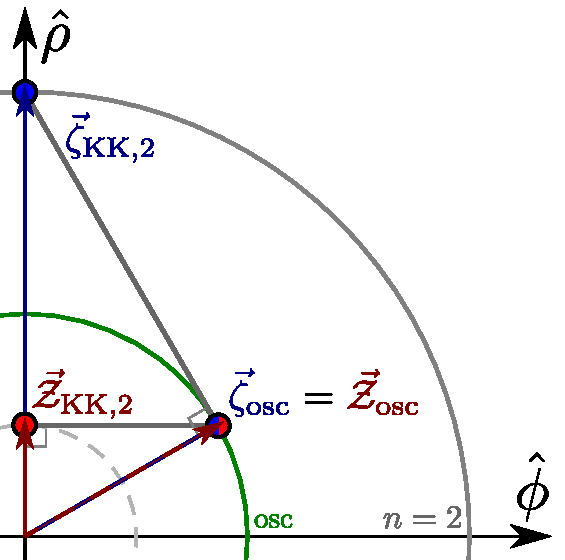
\includegraphics[width=0.4\textwidth]{species2.pdf}\label{sfig:KKstring}
		}
        \quad
	\subfigure[]{
			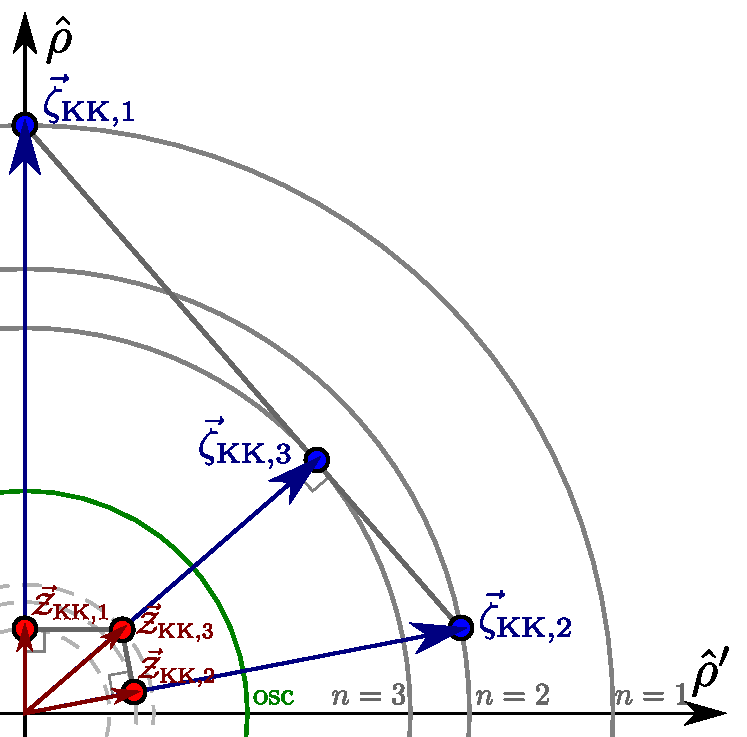
\includegraphics[width=0.4\textwidth]{species1.pdf}\label{sfig:twoKK}
		}
		\caption{\small Sketches depicting two possible scenarios in multi-field limits for maximal supergravity. For concreteness, we focus on $d=8$, with vectors associated to light towers in blue and to the species scale in red. \textbf{(a)} Decompactification of two internal dimensions and an emergent string limit. The species scale is controlled by the string scale unless we move along the pure decompactification direction, where it coincides with the ten-dimensional Planck mass. Here $\hat{\rho}$ and $\hat{\phi}$ denote the normalized radion and the ten-dimensional dilaton. \textbf{(b)} Two decompactification limits, of one and two internal dimensions, with towers $\vec{\zeta}_{{\rm KK},\, 1}$ and $\vec{\zeta}_{{\rm KK},\, 2}$ (as well as the total volume, $\vec{\zeta}_{{\rm KK},\, 3}$). Note that unless we decompactify a single cycle, the species scale is controlled by the eleven-dimensional Planck mass. The axes $\hat{\rho}$ and $\hat{\rho}'$ correspond to the normalized radions associated to decompactifying the 1- and 2-cycles, respectively.\label{fig:MT2radions} }
	\end{center}
\end{figure}
%%%%%%%%%%%%%%%%%%%%%%%%%%%%%%%%%%%%
	
	
\subsubsection*{Perturbative string limit}
	
This first scenario is characterized by having the species scale equal to the string scale. Hence, the $\mathcal{Z}$-vector of the species scale is the same than the $\zeta$-vector associated to the tower of string oscillator modes. However, this does not necessarily mean that the tower of string modes is the leading one. As we already know, if we have both a KK and a string tower becoming light, the species scale will indeed correspond to the string scale (even if the KK tower is parametrically lighter) as long as the string scale remains below the species scale associated to the KK tower (i.e. the higher dimensional Planck mass). Hence, the most general scenario with $\LSP \simeq m_s$ can contain both KK and string modes below the species scale. For the sake of concreteness, let us focus on the KK tower associated to the overall volume of the compactification space and the oscillator modes arising from a fundamental string already existing in the higher dimensional theory. We can then restrict to a slice of the tangent space of the moduli space spanned by the overall volume modulus $\hat{\rho}$ and the string dilaton $\hat{\phi}$. The relevant $\zeta$-vectors for such towers within this subspace are (in the flat frame $\{\hat{\phi},\hat{\rho}\}$, c.f. eqs. \eqref{eq:higherDdim}-\eqref{eq:chargetomasstower}) 
%
\begin{equation}\label{eq:zetasstringlimit}
	\begin{split} 
		\vec{\zeta}_{{\rm KK},\, n} &= \left( 0 , \sqrt{\frac{d+n-2}{n (d-2)}} \right)\, ,\quad \vec{\mathcal{Z}}_{{\rm KK},\, n} = \left( 0 , \sqrt{\frac{n}{(d+n-2) (d-2)}} \right)\, ,\\
		\vec{\zeta}_{\text{osc}}=\vec{\mathcal{Z}}_{\text{osc}} &= \left( \frac{1}{\sqrt{d+n-2}} , \sqrt{\frac{n}{(d+n-2)(d-2)}} \right)\, .
	\end{split}
\end{equation}
%
These vectors are plotted in Figure \ref{sfig:KKstring}. The tangent vectors of asymptotic geodesics in this slice of the moduli space are radial vectors (i.e straight lines passing through the origin) \cite{Etheredge:2022opl}. As explained in Section \ref{s:convexhull}, to obtain the exponential rate $\lambda$ of a tower (or the species scale) along a given geodesic, we just need to compute the projection of the associated $\zeta$-vector (resp. $\mathcal{Z}$-vector) along such direction. The larger this projection is, the fastest the mass (or the species scale) goes to zero asymptotically. The leading (i.e. the lightest) tower of states is therefore the one with the largest projection of $\vec\zeta$ over such direction; and the same applies to the species scale, which will be the one with the largest projection of $\vec{\mathcal{Z}}$.
	
If we move parallel to $\vec{\zeta}_{{\rm KK},\, n} $, both the Planck scale and the string scale decay at the same rate, so we can simply take the species scale vector as $\vec{\mathcal{Z}}_{{\rm KK},\, n}$. Otherwise, for any other intermediate direction, $\LSP$ will be given by the string scale, as it always remains below the Planck scale, so we should take instead $\vec{\mathcal{Z}}_{\text{osc}}$. On the other hand, the leading tower is always the KK one, except if we move parallel to $\vec{\zeta}_{\text{osc}}$, where both towers present the same exponential rate.\footnote{Note that precisely in this case the limit qualifies as equi-dimensional, in the notation defined in \cite{Lee:2019wij}. Such limits probe gravitational theories in the same number of spacetime dimensions as the starting point of the (infinite distance) trajectory. The fact that there is a KK tower decaying at the same rate than the string tower along this direction is also expected from the Emergent String Conjecture.} It is clear from Section \ref{s:patternintro} that $\vec{\zeta}_{\text{KK,}\, n} \cdot \vec{\mathcal{Z}}_{\text{KK},\, n}=\frac1{d-2}$ and $\vec{\zeta}_{\text{osc}} \cdot \vec{\mathcal{Z}}_{\text{osc}}=\frac1{d-2}$ for each tower independently, but it is less obvious that the pattern will continue working when considering both towers simultaneously. We find here that even in the case in which the species scale is the string scale and the leading tower corresponds to the KK tower, the pattern still holds:
%
\beq\label{eq:KKstring}
	\vec{\zeta}_{{\rm KK},\, n} \cdot \vec{\mathcal{Z}}_{\text{osc}}=\frac1{d-2}\, .
\eeq
%
This can be easily understood geometrically from Figure \ref{sfig:KKstring} as follows. Since $\vec{\mathcal{Z}}_{\text{osc}}$ is perpendicular to the convex hull generated by $\vec{\zeta}_{{\rm KK},\, n}$ and $\vec{\zeta}_{\rm osc}$, it turns out that $\vec{\zeta}_{\rm osc}$ is the projection of $\vec{\zeta}_{{\rm KK},\, n}$ along the direction associated to $\vec{\mathcal{Z}}_{\text{osc}}$, so that the pattern holds in general. Alternatively, the projection of $\vec{\mathcal{Z}}_{\text{osc}}$ along the direction determined by $\vec{\zeta}_{{\rm KK},\, n}$ coincides with $\vec{\mathcal{Z}}_{\text{KK,}\, n}$ since the radion component of $\vec{\mathcal{Z}}_{\text{osc}}$ arises from changing the masses to lower dimensional Planck units and it is therefore equal to the $\hat{\rho}$ component of $\vec{\mathcal{Z}}_{\text{KK},\, n}$, as can be seen from \eqref{eq:zetasstringlimit}. 
	
\subsubsection*{Decompactification limit}
	
The second scenario occurs when all the light towers below the species scale are KK modes (possibly decompactifying to different number of dimensions), and we do not find any additional tower of string modes before reaching the lightest higher dimensional Planck mass. Hence, the species scale is a Planck scale in higher dimensions. For concreteness, let us focus on a two-dimensional slice spanned by two KK towers decompactifying to $d+n$ and $d+n'$ dimensions, respectively, with associated volume moduli $\hat{\rho}$ and $\hat{\rho}'$. The $\zeta$-vectors are given by \cite{Etheredge:2022opl} 
%
\begin{equation}\label{eq:n&n'zetas}
	\begin{split} 
		\vec{\zeta}_{{\rm KK},\, n} &= \left( 0 , \sqrt{\frac{d+n-2}{n (d-2)}} \right)\, ,\\
		\vec{\zeta}_{{\rm KK},\, n'} &= \left( \sqrt{\frac{d+n+n'-2}{n' (d+n-2)}} ,\, \sqrt{\frac{n}{(d+n-2)(d-2)}} \right)\, .
	\end{split}
\end{equation}
%
Depending on the infinite distance trajectory that we explore, the species scale will correspond to the Planck scale of decompactifying $n$, $n'$ or $n+n'$ extra dimensions. The associated $\mathcal{Z}$-vectors are
%
\begin{equation}
	\begin{split} 
		\vec{\mathcal{Z}}_{{\rm KK},\, n} &= \left( 0 , \sqrt{\frac{n}{(d+n-2) (d-2)}} \right) \, ,\\
		\vec{\mathcal{Z}}_{{\rm KK},\, n'} &= \left( \sqrt{\frac{n'(d+n+n'-2)}{(d+n'-2)^2 (d+n-2)}} ,\, \frac{n'}{d-2+n'} \sqrt{\frac{n}{(d+n-2) (d-2)}} \right) \, ,\\
		\vec{\mathcal{Z}}_{{\rm KK},\, n+ n'} &= \left( \sqrt{\frac{n'}{(d+n-2) (d+n+n'-2)}},\, \sqrt{\frac{n}{(d+n-2) (d-2)}} \right) \, \label{eq:combinedZ}.
	\end{split}
\end{equation}
%
All these vectors are represented in Figure \ref{sfig:twoKK}. The species scale corresponds to the lightest Planck scale along any chosen infinite distance trajectory. Hence, it will always be given by $\vec{\mathcal{Z}}_{{\rm KK},\,  n+ n'}$ in the entire asymptotic regime unless we move parallel to either $\vec{\zeta}_{{\rm KK},\, n}$ or $\vec{\zeta}_{{\rm KK},\, n'}\,$, in which case it reduces to $\vec{\mathcal{Z}}_{{\rm KK},\, n}$ or $\vec{\mathcal{Z}}_{{\rm KK},\, n'}\,$, respectively. However, the leading tower corresponds to decompactifying only $n$ or $n'$ extra dimensions unless we move precisely parallel to $\vec{\mathcal{Z}}_{{\rm KK},\,  n+ n'}$. The latter case would physically correspond to an isotropic decompactification of both $n$- and $n'$-dimensional internal cycles, with an effective KK tower of charge-to-mass vector given by (c.f. eq. \eqref{eq:effectivezeta})
%
\beq
	\vec{\zeta}_{{\rm KK},\, n+ n'} = \left( \sqrt{\frac{n' (d+n+n'-2)}{(d+n-2) (n+n')^2}}, \sqrt{\frac{n (d+n+n'-2)^2}{(n+n')^2(d+n-2) (d-2)}} \right) \, .
\eeq
%
Again, the pattern is clearly satisfied whenever we move along the asymptotic trajectories determined by any of the individual KK towers (due to \eqref{eq:patternKKn}), but it also nicely holds for intermediate directions within the asymptotic regime, since 
%
\beq\label{eq:doubleKK}
	\vec{\zeta}_{{\rm KK},\, n} \cdot \vec{\mathcal{Z}}_{{\rm KK},\, n+ n'}= \vec{\zeta}_{{\rm KK},\, n'} \cdot \vec{\mathcal{Z}}_{{\rm KK},\,n+ n'} = \frac1{d-2}\, .
\eeq
%
Notice that such relation may be easily understood from geometrical considerations as follows. The species vector $\vec{\mathcal{Z}}_{{\rm KK},\, n+n'}$ appears to be always perpendicular to the convex hull generated by $\vec{\zeta}_{{\rm KK},\, n}$ and $\vec{\zeta}_{{\rm KK},\, n'}$ (see Figure \ref{sfig:twoKK}), such that they both project to $\vec{\zeta}_{{\rm KK},\,  n+n'}$ along the direction determined by the former. Alternatively, $\vec{\mathcal{Z}}_{{\rm KK},\,  n+n'}$ projects to $\vec{\mathcal{Z}}_{{\rm KK},\, n}$ (analogously $\vec{\mathcal{Z}}_{{\rm KK},\, n'}$) along the direction determined by $\vec{\zeta}_{{\rm KK},\, n}$ (respectively $\vec{\zeta}_{{\rm KK},\, n'}$), which may be understood again as coming from a change of Planck units in both cases, given the commutativity of the compactification process (see Appendix \ref{ap:generalities}).
	
\subsubsection*{Summary}
	
What can be learned from the two scenarios above? The species scale vector $\vec{\mathcal{Z}}$ always happens to be perpendicular to the convex hull of the light towers of states. Conversely, the leading scalar charge-to-mass vector $\vec{\zeta}_{\rm t}$ is orthogonal to the convex hull generated by the species vectors. This is a feature that holds in general for M-theory toroidal compactifications, as we already observed in Chapter \ref{ch:bounds}. In fact, such constraints are restrictive enough so as to ensure that, once we assume that the pattern \eqref{eq:pattern} is verified by any pair of collinear vectors $\vec{\zeta}$ and $\vec{\mathcal{Z}}$ (i.e. when both are associated to one and the same tower of states), then the pattern extends automatically to any other asymptotic limit of the moduli space.\footnote{For instance, if $\vec{\zeta}_{\rm t}$ is orthogonal to the convex hull generated by $\vec{\mathcal{Z}}_{\rm sp}$ (the total specie scale) and $\vec{\mathcal{Z}}_{\rm t}$ (the one obtained only from considering the leading tower), then satisfying $\vec{\zeta}_{\rm t}\cdot \vec{\mathcal{Z}}_{\rm t}=\frac1{d-2}$ guarantees that $\vec{\zeta}_{\rm t}\cdot \vec{\mathcal{Z}}_{\rm sp}=\frac1{d-2}$, as the difference between the two species scale vectors is given by a vector which is orthogonal to $\vec{\zeta}_{\rm t}$.}
	
Notice, however, that the same story does not apply immediately when the amount of supersymmetry preserved by our theory is reduced, since then the charge-to-mass and species vectors can `slide' (or jump) non-trivially depending on where we sit in moduli space, see Sections \ref{s:16supercharges} and \ref{s:8supercharges}. In any event, most of our efforts in the upcoming sections will be dedicated to show that, even in such cases, the pattern is still verified at any infinite distance boundary, and it does so in a way that can be easily understood from pictures similar to those shown in Figure \ref{fig:MT2radions} above.	
	
\subsection{Maximal supergravity in 9d}
\label{ss:9d}
	
Next, we will illustrate the above general scenarios in concrete examples, starting with the unique 9d $\mathcal{N}=2$ supergravity theory arising from compactifying M-theory on a two-dimensional torus. The $\zeta$-vectors for the towers of states in this particular set-up were already analyzed in \cite{Etheredge:2022opl}, whilst the species ones have been derived in the previous chapter. Here we will build upon these results and simply check if the pattern \eqref{eq:pattern} is verified, paying special attention to the way in which this happens.

Recall that the moduli space of M-theory on $\mathbf{T}^2$ is classically exact, it moreover presents a coset structure (c.f. \eqref{eq:9dmodspaceSSDC}) and is locally parametrized by the complex structure of the torus as well as the overall volume modulus. Per our discussion in Section \ref{ss:MthyT2SSDC}, we will forget in the following about the compact scalar field, since it seems to play no role whatsoever. We also use the basis \eqref{eq:canonicalnormalization} of canonically normalized fields $\{\hat U, \hat \tau \}$ to express any moduli-dependent quantity, including the relevant $\zeta$- and $\mathcal{Z}$-vectors.

As discussed in \cite{Etheredge:2022opl}, the relevant towers of states becoming light at the infinite distance limits of this moduli space are $\frac{1}{2}$-BPS particles. For this particular example, the convex hull determined by the scalar charge-to-mass vectors associated to all light towers is spanned by Kaluza-Klein modes with the following $\zeta$-vectors
%
\begin{equation}\label{eq:KKzetas9d}
	\vec{\zeta}_{\text{KK},\, 1} = \left( \frac{3}{\sqrt{14}},\frac{1}{\sqrt{2}} \right) \, , \qquad
	\vec{\zeta}_{\text{KK},\, 1'} = \left( \frac{3}{\sqrt{14}},-\frac{1}{\sqrt{2}}\right) \, ,
\end{equation}
%
as well as M2-branes wrapping the compactification manifold, with
%
\begin{equation}\label{eq:M2zeta9d}
	\vec{\zeta}_{\text{M2}} = \left( -\sqrt{\frac{8}{7}},0 \right) \, .
\end{equation}
%
We have adopted the notation $\vec{\zeta}=\left(\zeta^{\hat U}, \zeta^{\hat \tau} \right)$. Notice that they all satisfy the relation $|\vec{\zeta}|^2=8/7$, in accordance with eq. \eqref{eq:zeta&speciesveconemodulus} above for $d=9$ and $n=1$.
	
On the other hand, their associated species scale vectors, $\vec{\mathcal{Z}}$, were found to be
%
\begin{equation} \label{eq:SSvec9d}
	\begin{split} 
		\vec{\mathcal{Z}}_{\text{KK},\, 1} &= \left( \frac{3\sqrt{14}}{112},\frac{\sqrt{2}}{16} \right) \, , \qquad \vec{\mathcal{Z}}_{\text{KK},\, 1'} = \left( \frac{3\sqrt{14}}{112},-\frac{\sqrt{2}}{16}\right) \, ,\\
		\vec{\mathcal{Z}}_{\text{M2}} &= \left( -\frac{1}{2\sqrt{14}} , 0\right) \, ,
	\end{split}
\end{equation}
%
corresponding to the appropriate 10d Planck mass of the decompactified (dual) theories. %In particular, since $|\vec{\mathcal{Z}}|^2=\frac{1}{(d-1)(d-2)}=\frac{1}{56}$, these saturate the lower bound proposed in \cite{Calderon-Infante:2023ler} for the decay parameter, $\lambda_{\text{sp}}$, of the species scale.
	
Furthermore, as explained in Chapter \ref{ch:bounds}, a crucial ingredient when determining the set of all possible species scales is the concept of effective tower. Indeed, for intermediate directions between $\vec{\zeta}_{\text{KK},\, 1}$ and $\vec{\zeta}_{\text{KK},\, 1'}$, despite one KK tower being (in general) parametrically lighter than the other, one still needs to account for bound states thereof in order to properly compute the species scale in that asymptotic regime (see discussion around eq. \eqref{eq:conforeffectivetower}). Upon doing so, one arrives at the following species scale vector
%
\begin{equation}\label{eq:effectivespecies}
	\vec{\mathcal{Z}}_{{\rm KK},\, 2}=\frac{1}{9} \left( \vec{\zeta}_{{\rm KK},\, 1} +\vec{\zeta}_{{\rm KK},\, 1'} \right) = \left( \frac{\sqrt{14}}{21} , 0\right)\, ,
\end{equation}
%
to which we can associate an effective (averaged) mass scale and charge-to-mass vector as follows
%
\begin{equation}\label{eq:effectivemass}
	\vec{\zeta}_{{\rm KK},\,2}=\frac{1}{2} \left( \vec{\zeta}_{{\rm KK},\, 1} +\vec{\zeta}_{{\rm KK},\, 1'} \right) = \left( \frac{3}{\sqrt{14}} , 0\right)\, .
\end{equation}
%
The physical interpretation for \eqref{eq:effectivespecies} is clear --- it corresponds to the 11d Planck scale, whilst the charge-to-mass vector \eqref{eq:effectivemass} is a meaningful quantity only when one takes the decompactification limit in an isotropic way, namely for an asymptotic vector $\hat T = \partial_{\hat U}$. Still it may be useful to think in terms of `averaged' geometric quantities when computing the species scale vectors and checking the pattern \eqref{eq:pattern} explicitly, as we discuss later on in this section.
	
Apart from these, there is also another set of $\frac{1}{2}$-BPS states comprised by critical Type IIA strings arising from M2-branes wrapped on a non-trivial 1-cycle. Their oscillator modes were seen to lead to the following charge-to-mass vectors (c.f. eq. \eqref{eq:speciesscalevectorsstringsT2})
%
\begin{equation}\label{eq:9dstrings}
	\vec{\zeta}_{\text{osc}} = \left( -\frac{1}{2 \sqrt{14}},\frac{1}{2\sqrt{2}} \right) \, , \quad 
	\vec{\zeta}_{\text{osc'}} = \left( -\frac{1}{2 \sqrt{14}},- \frac{1}{2\sqrt{2}} \right) \, ,
\end{equation}
%
which coincide with those of their associated species scale and moreover satisfy $|\vec{\mathcal{Z}}_{\text{osc}}|^2=\frac{1}{d-2}=\frac{1}{7}$ (c.f. eq. \eqref{eq:zeta&speciesvecstring}).

In Figure \ref{fig:T2SDC&SSDC} we depict again the convex hulls associated to the towers of states along with their species scale vectors, which are constructed from the expressions \eqref{eq:KKzetas9d}-\eqref{eq:9dstrings}. Notice that there is a $\mathbb{Z}_2$-symmetry with respect to the $\hat \tau$-axis, which may be thought of as a discrete remnant of the U-duality group of the theory (more specifically it is given by its associated Weyl group, see footnote \ref{fnote.Weyl} below). Therefore, it is enough to focus just on the upper-half plane in order to check the condition \eqref{eq:pattern}.
	
First, notice that for those directions in which both $\vec{\zeta}_{\text{t}}$ and $\vec{\mathcal{Z}}_{\text{sp}}$ are aligned, namely when $\hat T$ is parallel to the vector $\vec{\zeta}_I$ associated to any leading tower, the condition $\vec{\zeta}_{\text{t}} \cdot \vec{\mathcal{Z}}_{\text{sp}}= \frac{1}{d-2} =\frac{1}{7}$ is satisfied. Moreover, this turns out to be sufficient for the pattern to hold also along intermediate directions. The reason behind is a duality between both convex hull diagrams. In fact, as one can see from Figure \ref{fig:T2SDC&SSDC}, the vertices from one correspond to edges of the other and viceversa, the latter being orthogonal to the former. Therefore, it follows that whenever we take $\vec{\zeta}_{\text{t}}$ (analogously $\vec{\mathcal{Z}}_{\text{sp}}$) to be given by any of the two vertices generating an edge of its corresponding diagram, its inner product with the dual $\vec{\mathcal{Z}}_{\text{sp}}$ (analogously $\vec{\zeta}_{\text{t}}$) orthogonal to such edge reduces to that of the previous `parallel' cases and thus satisfies the pattern \eqref{eq:pattern}.
	
%%%%%%%%%%%%
\begin{figure}[htb]
	\begin{center}
		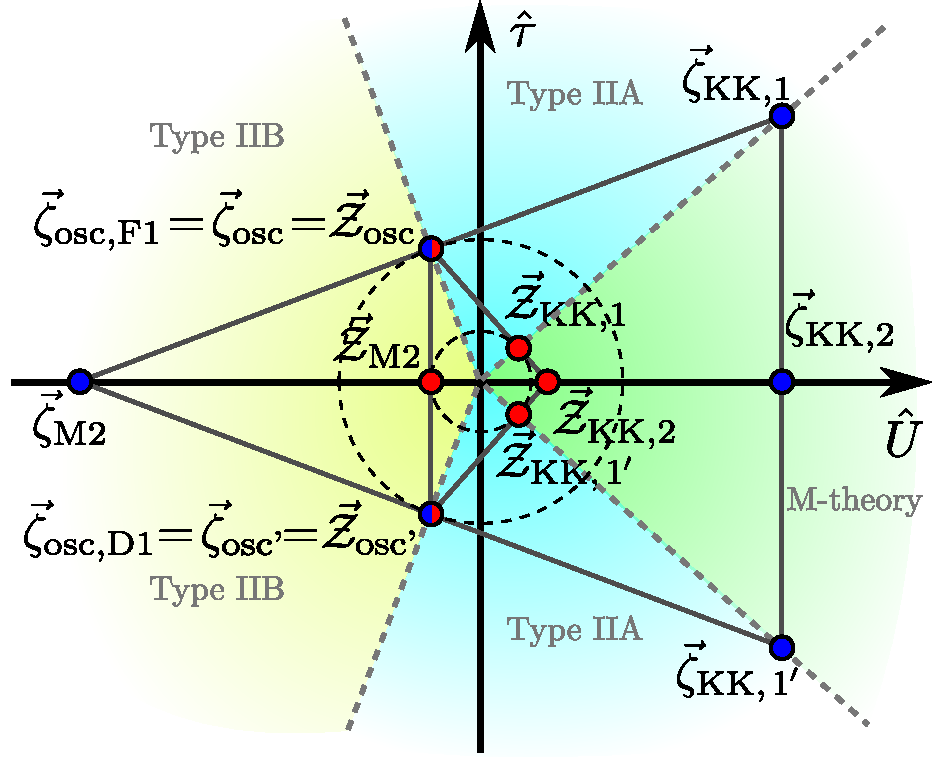
\includegraphics[scale=.55]{MaxSugra9dNEW.pdf}
		\caption{\small Convex hulls spanned by the species scale (red) and mass scales of the leading towers (blue) in nine-dimensional maximal supergravity. The 1-spheres of radii $\frac{1}{\sqrt{d-2}}=\frac{1}{\sqrt{7}}$ and $\frac{1}{\sqrt{(d-1)(d-2)}}=\frac{1}{\sqrt{56}}$ are plotted in dashed lines. We also depict the different duality frames of the theory using distinct shades. Notice that both Type IIA and Type IIB string theory have two different duality frames, whereas there is a single one for M-theory.} 
		\label{fig:T2SDC&SSDC}
	\end{center}
\end{figure}
%%%%%%%%%%%%
	
	
\subsection{Maximal supergravity in 8d}
\label{ss:8d}
	
As our second example, we now take M-theory compactified on a $\mathbf{T}^3$, leading to 8d $\mathcal N=2$ supergravity, whose bosonic action was already discussed in Section \ref{ss:8dmaxsugra}. However, instead of choosing a parametrization which makes the U-duality group manifest, we take here the same approach as in Section \ref{ss:MthyT3SSDC} and consider the 9d theory from the previous example compactified on an additional circle, leading to eq. \eqref{eq:8dalternativeaction}. We will forget again about the axion fields, and moreover fix some convenient basis $\{ \hat U, \hat \tau, \hat \rho\}$ of canonically normalized saxions (see discussion around eq. \eqref{eq:8dcanonical}), which allows us to read off most of the scalar charge-to-mass vectors characterizing the infinite towers of states from the previous 9d example.\footnote{This procedure is explained in detail in Appendix \ref{ap:generalities}.} Therefore, for the KK towers one obtains
%
\begin{equation}
	\begin{split} 
		\vec{\zeta}_{\text{KK},\, 1} &= \left( \frac{1}{\sqrt{2}} , \frac{1}{\sqrt{42}}, \frac{3}{\sqrt{14}} \right) \, , \qquad \vec{\zeta}_{\text{KK},\, 1'} = \left( -\frac{1}{\sqrt{2}} , \frac{1}{\sqrt{42}}, \frac{3}{\sqrt{14}} \right) \, ,\\
		\vec{\zeta}_{\text{KK},\, 1''} &= \left( 0 , \sqrt{\frac{7}{6}}, 0 \right) \, ,
	\end{split}
\end{equation}
%
where the last $\zeta$-vector arises from the extra $\mathbf{S}^1$ and the notation is $\vec{\zeta}=\left(\zeta^{\hat \tau}, \zeta^{\hat \rho}, \zeta^{\hat U}\right)$. Analogously, one finds a triplet of towers comprised by M2-branes wrapping different 2-cycles within $\mathbf{T}^3$, with the following charge-to-mass vectors
%
\begin{equation} \label{eq:M2vectorspattern}
	\begin{split} 
		\vec{\zeta}_{\text{M},\, 1} &= \left( \frac{1}{\sqrt{2}} , -\frac{5}{\sqrt{42}}, -\frac{1}{\sqrt{14}} \right) \, , \qquad \vec{\zeta}_{\text{M},\, 1'} = \left( -\frac{1}{\sqrt{2}} , -\frac{5}{\sqrt{42}}, -\frac{1}{\sqrt{14}} \right) \, ,\\
		\vec{\zeta}_{\text{M},\, 1''} &= \left( 0, \frac{1}{\sqrt{42}}, -\sqrt{\frac{8}{7}} \right)  \, ,
	\end{split}
\end{equation}
%
where the last one is inherited from the 9d set-up, whilst the first two are new (c.f. Table \ref{tab:BPSstates}). %we denote as $\vec{\zeta}_{\text{M},\, i}$ the corresponding vector associated to the tower of M2-branes wrapping the cycle labeled by $(j, k)$ (with $i, j, k=1, 2, 3$) such that $\epsilon_{ijk}=1$ \cite{Calderon-Infante:2023ler}. 
Notice that these vectors already generate the convex hull associated to the light towers, see Figure \ref{sfig:mass8d}. However, there also exist additional towers of states corresponding to the oscillation modes of critical (Type IIA) strings, whose $\zeta$-vectors read as
%
\begin{equation} \label{eq:stringvectorspattern}
	\begin{split} 
		\vec{\zeta}_{\text{osc}} &= \left( \frac{1}{2\sqrt{2}} , \frac{1}{\sqrt{42}}, -\frac{1}{2 \sqrt{14}} \right) \, , \qquad \vec{\zeta}_{\text{osc}'} = \left( -\frac{1}{2\sqrt{2}} , \frac{1}{\sqrt{42}}, -\frac{1}{2 \sqrt{14}} \right) \, ,\\
		\vec{\zeta}_{\text{osc}''} &= \left( 0 , -\sqrt{\frac{2}{21}}, \frac{1}{\sqrt{14}} \right)  \, ,
	\end{split}
\end{equation}
%
and which happen to lie at the extremal ball, thus saturating the sharpened Distance Conjecture \cite{Etheredge:2022opl}. The first two are inherited from the 9d example above (c.f. \eqref{eq:9dstrings}), whilst the third one arises from the M2-brane of 11d supergravity wrapped along the additional circle.
	
One can analogously compute the species scale vectors within each asymptotic direction of the 8d moduli space. This exercise was already performed in Section \ref{ss:MthyT3SSDC}, so we refrain from repeating it here and refer the reader interested in the details to that section. The resulting $\mathcal{Z}$-vectors are displayed in eqs. \eqref{eq:stringvectors}-\eqref{eq:KK&M2vectorscombined}, leading to the convex hull diagram shown in Figure \ref{sfig:species8d}. 

%%%%%%%%%%%%%%%%%%%%%%%%%%%%%%%%%%%%
\begin{figure}
	\begin{center}
\subfigure[]{
				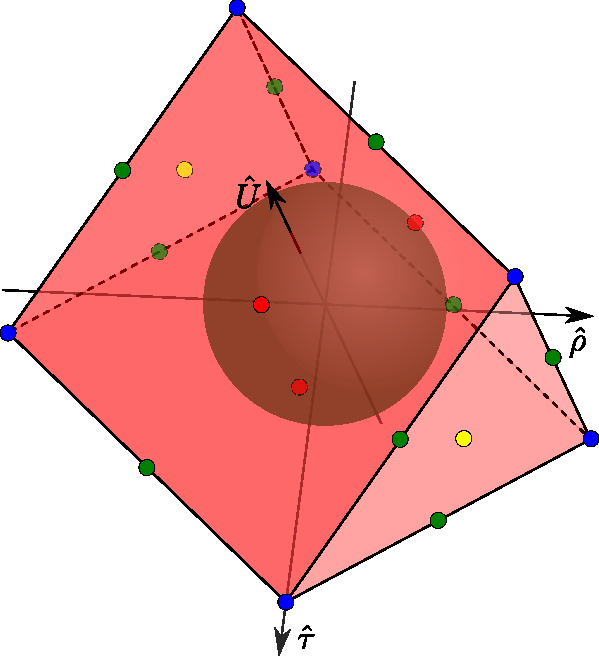
\includegraphics[width=0.45\textwidth]{MaxSugra8d.pdf}\label{sfig:mass8d}
			}
            \quad
			\subfigure[]{
				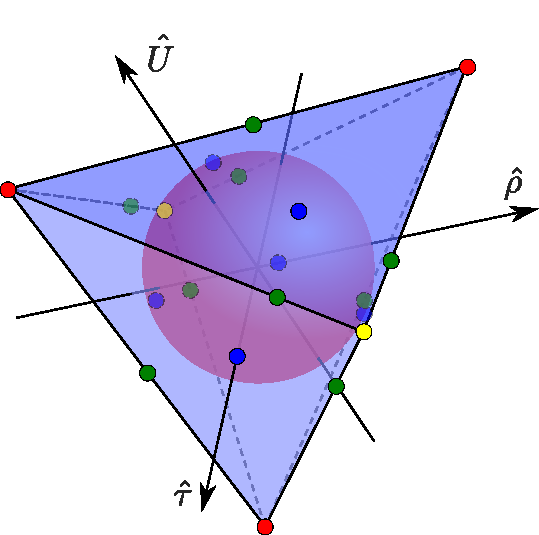
\includegraphics[width=0.45\textwidth]{MaxSugra8d-species.pdf}\label{sfig:species8d}
			}
			\caption{\small Convex hull conditions for the masses $\{\vec{\zeta}_I\}$ \textbf{(a)} and species scales $\{\vec{\mathcal{Z}}_J\}$ \textbf{(b)} of the leading towers in eight-dimensional maximal supergravity, containing the `extremal balls' of radii $\frac{1}{\sqrt{d-2}}=\frac{1}{\sqrt{6}}$ and $\frac{1}{\sqrt{(d-1)(d-2)}}=\frac{1}{\sqrt{42}}$, respectively. The string towers are depicted in red \fcolorbox{black}{red}{\rule{0pt}{6pt}\rule{6pt}{0pt}}, whilst KK towers associated to decompactification of one, two and three dimensions appear in blue \fcolorbox{black}{blue}{\rule{0pt}{6pt}\rule{6pt}{0pt}}, green \fcolorbox{black}{dark-green}{\rule{0pt}{6pt}\rule{6pt}{0pt}} and yellow \fcolorbox{black}{yellow}{\rule{0pt}{6pt}\rule{6pt}{0pt}}, respectively. Note that the string vectors coincide in the two diagrams.}\label{fig:convexhulls8d}
	\end{center}
\end{figure}
%%%%%%%%%%%%%%%%%%%%%%%%%%%%%%%%%%%%

In order to check whether the condition \eqref{eq:pattern} is satisfied or not, one can proceed as in the 9d example above and focus --- thanks to the U-duality group of the theory --- on a strictly smaller polyhedron. Indeed, since the symmetry group of the convex polytope is $\mathsf{S_2}\times \mathsf{S_3}$, it is enough for our purposes to take 1/12 of the full diagram, namely the one containing e.g., the set $\lbrace \vec{\zeta}_{\text{KK},\, 1''}, \vec{\zeta}_{\text{osc}}, \vec{\zeta}_{\text{KK-M},\,2}, \vec{\zeta}_{{\rm KK},\, 2'}, \vec{\zeta}_{{\rm KK},\, 3}\rbrace$. Figure \ref{fig:sym} depicts the aforementioned vertices and the fundamental domain they span, as well as the discrete symmetries associated to the diagram. One can now easily check that along these particular directions, the product $\vec{\zeta}_{\text{t}} \cdot \vec{\mathcal{Z}}_{\text{sp}}= \frac{1}{d-2} =\frac{1}{6}$ is verified, since the species scale and the charge-to-mass vectors are aligned. Furthermore, as it was also the case in our previous example, this is actually all we need to check in order to get convinced that the pattern holds along every other intermediate asymptotic direction as well. This follows again from the fact that the vertices spanning one convex hull are orthogonal to the faces of the other and viceversa, see Figure \ref{fig:convexhulls8d}.
	
%%%%%%%%%%%%
\begin{figure}[htb]
	\begin{center}
		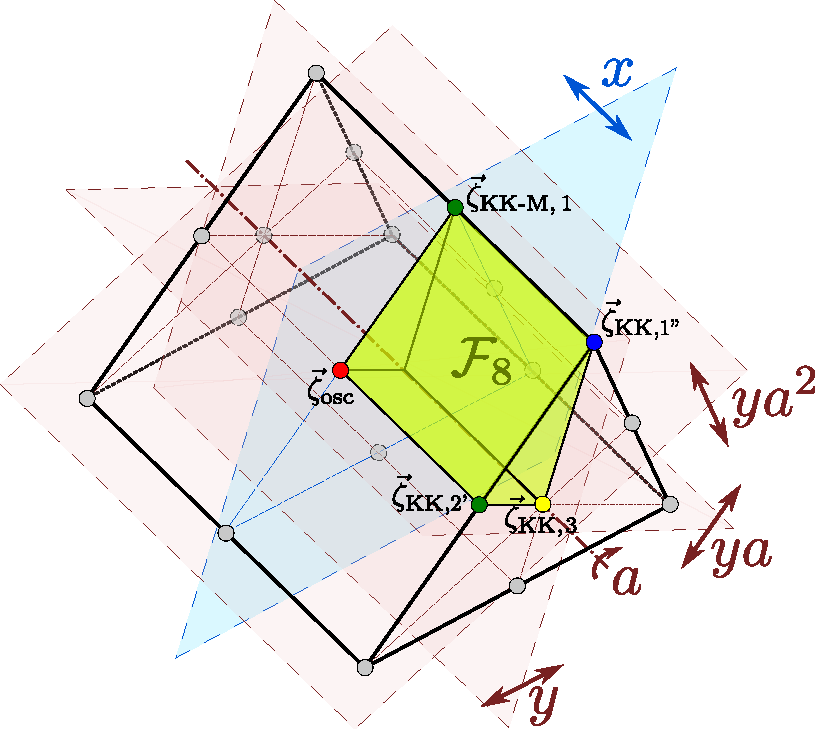
\includegraphics[scale=.7]{MaxSugra8d-s.pdf}
		\caption{\small Sketch of the fundamental domain $\mathscr{F}_8$ of the $\mathsf{S_3}\times \mathsf{S_2}=\left \langle y,\,a: y^2=a^3=e,\, yay=a^{-1} \right\rangle\times\left\langle x: x^2=e\right\rangle$ symmetry group acting on the scalar charge-to-mass vectors associated to the relevant towers in 8d maximal supergravity. The figure also shows the towers spanning the fundamental domain as well as the individual actions of the symmetry group. A completely analogous fundamental domain for the species scale polytope from Figure \ref{sfig:species8d} can be built, since both $\{\vec{\zeta}_I\}$ and $\{\vec{\mathcal{Z}}_J\}$ present the same symmetries.} 
		\label{fig:sym}
	\end{center}
\end{figure}
%%%%%%%%%%%%
	
\subsection{Maximal supergravity in $d<8$}
\label{ss:generaldim}
	
After the previous concrete examples, we will argue in what follows that the results discussed there hold more generally in the context of maximal supergravity. The strategy will be to isolate the key ingredients from the nine- and eight-dimensional set-ups and translate them into the more general case in $d$ spacetime dimensions. This is done in Section \ref{sss:sketch}, whilst the computational details are relegated to Section \ref{sss:generalcomputations}.
	
\subsubsection{A sketch of the proof}
\label{sss:sketch}
	
The argument proceeds in a recursive manner, relying essentially on the duality properties of the theory as well as the uniqueness of maximal supergravity for $d\leq9$. 
	
Let us start by noticing from the examples above that the charge-to-mass vectors associated to towers with density parameter $n$ lie always along a facet\footnote{Actually, they are located at the point of the facet closest to the origin.} of the convex hull polytope with \emph{dimension} equal to $n-1$ (see Figures \ref{fig:T2SDC&SSDC} and \ref{sfig:mass8d}), whilst those vectors controlling the species scale belong to a facet of \emph{codimension} $n$ (c.f. Figures \ref{fig:T2SDC&SSDC} and \ref{sfig:species8d}).\footnote{The vectors associated to string towers appear at facets of maximal (co-)dimension for the charge-to-mass (resp. species) diagram.} This holds in lower spacetime dimensions as well, since the length of the vectors is fully determined once $d$ and $n$ are specified (c.f. \eqref{eq:zeta&speciesveconemodulus}), and it is indeed a  clear manifestation of the duality between both convex hulls in the sense that the facets of one correspond to the vertices of the other, and viceversa. 
	
One also notices that the diagrams present some symmetry properties that reflect the U-duality group of the quantum theory (see Table \ref{tab:irreps} below). This, in turn, allows us to restrict ourselves to some \emph{fundamental domain}, i.e. a subset of the original convex hull containing all the relevant information for the diagram, whilst the remaining parts of the hull appear to be mere copies of the former, obtained upon acting with the different elements of the symmetry group. In fact, one may view such fundamental domain as the region whose boundaries precisely arise as fixed submanifolds under some element(s) of the symmetry group, which moreover coincides with the Weyl subgroup associated to the U-duality group (see Figure \ref{fig:sym}).\footnote{\label{fnote.Weyl}Consider some EFT with a $n$-dimensional moduli space $\mathcal{M}_{\rm mod}$ parametrized by the scalars $\{\varphi^i\}$, $i=1, \ldots, n$. The U-duality group $G$ of said theory transforms the scalars $\{\varphi^i\}$ in a way such that the different states of the EFT are mapped to one another. However, if we are interested only in non-compact scalars (thus ignoring compact axionic fields), some of the transformations of $G$ might affect only the compact ones, which we left fixed. These transformations are the elements of a \emph{maximal torus of $G$, $T_G\hookrightarrow G$}, which is the maximal Abelian, connected and compact subgroup of $G$. As in general $T_G$ is not a normal subgroup of $G$, in order to properly quotient $G$ by $T_G$, one introduces the normalizer $N_G (T_G)=\{g\in G:gT_G=T_Gg\}$, corresponding to the largest subgroup of $G$ such that $T_G$ is a normal subgroup. Then the \emph{Weyl group} of $G$ is defined as ${\rm W(G)}:=N_G(T_G)/T_G$, and it will correspond to the symmetries of the non-compact scalars (and thus of the different vectors under consideration). ${\rm W(G)}$ is then some finite (there are only so many ways of exchanging points) subgroup of $\mathsf{GL(\mathbb{R}^{k})}$, where $k\leq n$ is the number of unbounded moduli.}
	
Therefore, what we need first to know is how to select a fundamental domain $\mathscr{F}_d$, in practice. For this, we note that the towers of states with $n=1$ arrange themselves into a \emph{single} irreducible representation of the U-duality group for $d<9$, as shown in the second column of Table \ref{tab:irreps}. These include perturbative (i.e. KK, winding modes, etc.) as well as non-perturbative states (wrapped branes, KK-monopoles, etc.), and for us it will be enough to focus on just one of them, which we take to be of perturbative nature, namely a Kaluza-Klein vector. Hence, we work inductively, starting from M-theory compactified on $\mathbf{T}^k$ down to $d+1=11-k$ dimensions, where we assume the pattern \eqref{eq:pattern} to hold. Then, we dimensionally reduce on an extra circle, leading to M-theory on $\mathbf{T}^k \times \mathbf{S}^1 \cong \mathbf{T}^{k+1}$, and we consider the cone of asymptotic directions comprised by the large radius direction (of the additional $\mathbf{S}^1$) and the KK replica of the vectors determining some fundamental domain, $\mathscr{F}_{d+1}$, in the parent $(d+1)$-dimensional theory. %\footnote{In fact, this typically overcounts the number of necessary vectors to determine the fundamental region (c.f. Figure \ref{fig:sym}), since one needs to take into account the redundancies already present in the EFT coming from the $\mathbf{T}^k$ reduction of M-theory.}
Upon doing so, one can easily check (see Section \ref{sss:generalcomputations} below) that eq. \eqref{eq:pattern} is verified along any asymptotic trajectory within $\mathscr{F}_d$. Finally, since the pattern has already been shown to hold for $k=1,2,3$ (corresponding to maximal supergravity in ten, nine and eight dimensions, respectively), one concludes that it extends to all lower dimensional cases as well.
	
%%%%%%%%%%%%%%%%%%%%%%%%%%%%%%%
\begin{table}[h!!]\begin{center}
		\renewcommand{\arraystretch}{1.00}
		\begin{tabular}{|c|c|c|c|c|}
			\hline
			$d$ &  U-duality group  & Irrep. &  $\{\vec{\zeta}_I\}$ sym. group & Order\\
			\hline 
                \hline
			10A & 1  & $\mathbf{1}$ & 1 & 1 \\
			10B & $\mathsf{SL(2,\mathbb{Z})}$  & $\mathbf{2}$ & $\mathbb{Z}_2 \simeq \mathsf{S_2}$ & 2 \\
			9 & $\mathsf{SL(2,\mathbb{Z})}$   & $\mathbf{2} \oplus \mathbf{1}$ & $\mathbb{Z}_2 \simeq \mathsf{S_2}$ & 2 \\
			8 & $\mathsf{SL(2,\mathbb{Z})} \times \mathsf{SL(3,\mathbb{Z})}$  & $(\mathbf{2},\mathbf{3} )$ & $\mathsf{S_2}\times \mathsf{S_3}$ & 12 \\
			7 & $\mathsf{SL(5,\mathbb{Z})}$  & $\mathbf{10}$ & $\mathsf{S_5}$ & 120 \\
			6 & $\mathsf{SO(5, 5, \mathbb{Z})}$  & $\mathbf{16}$ & $\mathsf{\text{W}\, (Spin(5,5))}$ & $1\,920$ \\
			5 & $\mathsf{E_{6 (6)} (\mathbb{Z})}$  & $\mathbf{27}$ & $\mathsf{\text{W}\, (E_6)}$ & $51\,840$ \\
			4 & $\mathsf{E_{7 (7)} (\mathbb{Z})}$  & $\mathbf{56}$ & $\mathsf{\text{W}\, (E_7)}$ & $2\,903\,040$ \\
			3 & $\mathsf{E_{8 (8)} (\mathbb{Z})}$  & $\mathbf{248}$ & $\mathsf{\text{W}\, (E_8)}$ & $719\,953\,920$ \\
				\hline
		\end{tabular}
		\caption{\small U-duality representations of the particle multiplets in M-theory on $\mathbf{T}^{k}$ \cite{Obers:1998fb} for $10\geq d\geq 3$. Note that there are two possibilities for $d=10$, corresponding to ten-dimensional Type IIA and Type IIB supergravities. The second column shows the vector and charge representations for $n=1$ BPS towers, which for $d<9$ arrange into a single irrep. Additionally, the symmetry group acting on the $\zeta$ (equivalently $\mathcal{Z}$)-vectors is displayed, which corresponds to the Weyl subgroup of the associated U-duality group, as well as its finite order \cite{wilson2009finite}. The latter controls the number of copies of $\mathscr{F}_d$ that comprise the convex hull of $\zeta$- or $\mathcal{Z}$-vectors.}
		\label{tab:irreps}
	\end{center}
\end{table}
%%%%%%%%%%%%%%%%%%%%%%%%%%%%%%%%%
	
\subsubsection{Relevant computations}
\label{sss:generalcomputations}
The aim of this subsection is to provide some of the details that corroborate our previous claims regarding the analysis of the pattern \eqref{eq:pattern} in $d<8$ maximal supergravity. Let us assume that we have already fixed a fundamental domain $\mathscr{F}_d$, as outlined in Section \ref{sss:sketch}. Such polytope is thus generated by the reference $n=1$ tower, with charge-to-mass vector $\vec{\zeta}_{\rm KK, 1}$, together with the KK replica of those vectors determining the fundamental domain of the theory in one dimension higher (see Figure \ref{fig:sym}). In the following, we will denote the latter as $\lbrace \vec{\zeta}_{{\rm KK,}\,n+1} \rbrace$, with $n\in\{1,\ldots,10-d,\infty\}$. 
First, we notice that whenever we focus on a given direction determined by some $\vec{\zeta}$ within $\mathscr{F}_d$, the pattern is automatically satisfied, since both the species and charge-to-mass vectors are associated to one and the same tower and thus parallel to each other (c.f. \eqref{eq:patternKKn}). The non-trivial task is to show that eq. \eqref{eq:pattern} is still satisfied along intermediate directions as well, where the vectors $\lbrace \vec{\zeta}_{\text{t}}, \vec{\mathcal{Z}}_{\text{sp}}\rbrace$ are no longer aligned. %For intermediate directions one finds that, given that the faces of one hull are orthogonal to the vertices of the other, the relation $\vec{\zeta}_{\text{t}} \cdot \vec{\mathcal{Z}}_{\text{sp}}= \frac{1}{d-2}$ is verified for the lightest tower(s) becoming massless along the limit.
To do so, we first prove the following claim:
%
\begin{theorem}\label{claim1}
	The leading tower of states within $\mathscr{F}_d$ always corresponds to $\vec{\zeta}_{\rm KK,\, 1}$. Additional towers $m_I$ can become light at the same rate along certain asymptotically geodesic trajectories, characterized by some normalized tangent vector $\hat{T}$.
\end{theorem}
%
This can be easily shown upon computing the inner product between $\vec{\zeta}_{\rm KK,\, 1}$ and any other charge-to-mass vector belonging to the set $\lbrace \vec{\zeta}_{{\rm KK,}\,n+1} \rbrace$. One finds %\footnote{Notice that when $n \to \infty$, $\vec{\zeta}_{\text{KK,}n+1}$ collapses to $\vec{\zeta}_{\text{KK,}n}$, in agreement with the fact that the combined species scale of a fundamental string and any other KK tower is controlled solely by the former.}
%
\begin{equation}\label{eq:proofKK1dominant}
	\vec{\zeta}_{\rm KK,\, 1} \cdot \vec{\zeta}_{\text{KK},\, n+1} = \vec{\zeta}_{\rm KK, 1} \cdot \left[\frac{1}{n+1} \left( \vec{\zeta}_{\rm KK,\, 1} + n\, \vec{\zeta}_{{\rm KK,}\, n} \right) \right] = \frac{d+n-1}{(d-2) (n+1)} = |\vec{\zeta}_{{\rm KK},\, n+1}|^2\, ,
\end{equation}
%
where we have used eq. \eqref{eq:effectivezeta} in the second equality. The fact that it coincides with $|\vec{\zeta}_{{\rm KK},\, n+1}|^2$ implies, geometrically, that the segment of the hull determined by both vectors is indeed orthogonal to $\vec{\zeta}_{{\rm KK},\, n+1}$ itself (see e.g., Figure \ref{fig:MT2radions}). Now, given any normalized tangent vector $\hat{T}$, we can split it into parallel and perpendicular components with respect to the plane spanned by $\vec{\zeta}_{\rm KK,\, 1}$ and $\vec{\zeta}_{\text{KK,}\, n+1}$, such that $\hat{T}=\hat{T}^\parallel+\hat{T}^\perp$, where $\hat{T}^{\parallel}=a\,\vec{\zeta}_{\rm KK,\, 1}+b\,\vec{\zeta}_{\text{KK,}\, n+1}$, and with $a,\,b\geq 0$. Therefore, we have
%
\begin{align}
	\hat{T}\cdot(\vec{\zeta}_{\rm KK,\, 1} - \vec{\zeta}_{\text{KK},\, n+1})&=\hat{T}^\parallel\cdot(\vec{\zeta}_{\rm KK,\, 1} - \vec{\zeta}_{{\rm KK},\, n+1})\notag\\
	&=a\, \vec{\zeta}_{\rm KK,\, 1}\cdot(\vec{\zeta}_{\rm KK,\, 1} - \vec{\zeta}_{{\rm KK},\, n+1})+ b\,\vec{\zeta}_{{\rm KK},\, n+1}\cdot(\vec{\zeta}_{\rm KK,\, 1} - \vec{\zeta}_{{\rm KK},\, n+1})\notag\\
	&=a\,\underbrace{(|\vec{\zeta}_{{\rm KK},\, 1}|^2-|\vec{\zeta}_{{\rm KK},\, n+1}|^2)}_{>0}\geq 0,
\end{align}
%
so that the $\vec{\zeta}_{\rm KK,\, 1}$ tower always becomes light faster than $\vec{\zeta}_{\text{KK},\, n+1}$ except for $a=0$, namely when $\hat{T}^{\parallel} \propto \vec{\zeta}_{\text{KK},\, n+1}$, in which case they do so at the same rate. %This is the case for any asymptotic direction. Notice that this would not have been the case if the angle subtended between the two had been slightly bigger.
This ends our proof of Claim \ref{claim1} above.
On the other hand, the species scale strongly depends on the chosen asymptotic trajectory (see e.g., Figure \ref{fig:convexhulls8d}). Hence, in order to check the pattern \eqref{eq:pattern}, one needs to demonstrate the following statement:
%
\begin{theorem}\label{claim2}
	For any possible species scale vector spanning $\mathscr{F}_d$, that we collectively denote $\lbrace \vec{\mathcal{Z}}_{\rm{KK,}\,n+1} \rbrace$ with $n\in\{1,\ldots,10-d,\infty\}$, we find:
	\begin{subequations}
		\begin{equation}\label{eq:claim2a}
			\vec{\zeta}_{\rm{KK,}\, 1} \cdot \vec{\mathcal{Z}}_{\rm{KK},\, n+1} = \frac{1}{d-2}\, ,
		\end{equation}
		\begin{equation}\label{eq:claim2b}
		\vec{\zeta}_{\rm{KK},\, n'+1} \cdot \vec{\mathcal{Z}}_{\rm{KK},\, n+1}=\frac{1}{d-2}\, .
		\end{equation}
	\end{subequations}
In particular, the second equality holds provided the parent vectors satisfy the pattern in the higher $(d+1)$-dimensional theory. % it is assumed that $\vec{\zeta}_{\rm{KK},\, n'+1} \cdot \vec{\mathcal{Z}}_{\rm{KK},\, n+1} >0$.
\end{theorem}
%
Note that the first part of the claim above trivially follows from eqs. \eqref{eq:eff-vector} and \eqref{eq:proofKK1dominant}. The second statement, however, requires a bit more work. Intuitively, it means that the condition \eqref{eq:pattern} is consistent (or preserved) under dimensional reduction. %Intuitively, it should hold since, as shown in Claim \ref{claim1}, namely eq. \eqref{eq:claim2b} This phenomenom was already observed in the 9d and 8d examples above, and we aim here to show that it remains true in lower dimensional set-ups as well. 
Thus, we take, without loss of generality, some vector $\vec{\mathcal{Z}}_{\text{KK},\, n+1}$ as the one dominating certain asymptotic region of moduli space within the fundamental domain, and we consider the inner product \eqref{eq:claim2b}. Here, $\vec{\zeta}_{\text{KK},\, n'+1}$ is taken to be any other charge-to-mass vector within $\mathscr{F}_d$ such that it verifies the pattern with respect to $\vec{\mathcal{Z}}_{\text{KK},\, n+1}$ in the parent $(d+1)$-dimensional theory. Recall that, upon dimensionally reducing some vectors $\vec{\zeta}^{\,(d+1)}_{\text{KK},\, n'}$ and $\vec{\mathcal{Z}}^{\,(d+1)}_{\text{KK},\, n}$ on a circle, one gets (c.f. Section \ref{s:consistencydimreduc})
%
\begin{align}
	\vec{\zeta}_{\text{KK},\, n'} = \left( \vec{\zeta}^{\,(d+1)}_{\text{KK},\, n'}\, ,\, \frac{1}{\sqrt{(d-1)(d-2)}}\right)\, , \quad  \vec{\mathcal{Z}}_{\text{KK},\, n+1} = \left( \vec{\mathcal{Z}}^{\,(d+1)}_{\text{KK},\, n}\, ,\, \frac{1}{\sqrt{(d-1)(d-2)}}\right)\, ,
\end{align}
%
where the first components of both vectors are directly inherited from the ones of the theory in $d+1$ dimensions, whilst the last entry corresponds to the $\mathbf{S}^1$ radion direction (see also Appendix \ref{ap:generalities}). Hence, requiring $\vec{\zeta}_{\text{KK},\, n'+1}$ to verify the pattern in the higher-dimensional theory translates into the following statement
%
\begin{equation}\label{eq:patternd+1}
	\vec{\zeta}^{\,(d+1)}_{\text{KK},\, n'} \cdot \vec{\mathcal{Z}}^{\,(d+1)}_{\text{KK},\, n} = \frac{1}{d-1}\, ,
\end{equation}
%
such that we finally obtain
%
\begin{align}
	\vec{\zeta}_{\text{KK},\, n'+1} \cdot \vec{\mathcal{Z}}_{\text{KK},\, n+1} &= \left[\frac{1}{n'+1} \left( \vec{\zeta}_{\text{KK},\, 1} + n'\, \vec{\zeta}_{\text{KK},\, n'} \right) \right] \cdot \vec{\mathcal{Z}}_{\text{KK},\, n+1} \notag\\
	& = \frac{1}{n'+1} \vec{\zeta}_{\text{KK},\, 1} \cdot \vec{\mathcal{Z}}_{\text{KK},\, n+1} + \frac{n'}{n'+1} \left[ \vec{\zeta}^{\,(d+1)}_{\text{KK},\, n'} \cdot \vec{\mathcal{Z}}^{\,(d+1)}_{\text{KK},\, n} + \frac{1}{(d-1)(d-2)}\right] \notag\\
	&=\frac{1}{d-2}\, ,
\end{align}
%
where in order to arrive at the last equality one needs to use eqs. \eqref{eq:claim2a} and \eqref{eq:patternd+1} above. This completes the proof of Claim \ref{claim2}, which ensures that both convex hull diagrams, namely that associated to the $\zeta$-vectors and the species one, are completely dual to each other (with respect to a sphere of radius $\frac{1}{\sqrt{d-2}}$), as also happened for the 9d and 8d cases. Therefore, according to our discussion in Section \ref{sss:sketch}, the immediate consequence of this is that the pattern \eqref{eq:pattern} holds in complete generality for flat space compactifications with maximal supergravity.

For completeness, let us mention that this property holds as well between vectors in- and outside the selected fundamental region (see e.g., Figures \ref{fig:T2SDC&SSDC} and \ref{fig:convexhulls8d}). Notice that this follows from the analysis restricted to $\mathscr{F}_d$ just performed, since any vector outside the fundamental domain can be reached from another one within the latter via the action of some element $g\in G$ of the finite symmetry group $G$ of the diagram. However, since $G$ is a subgroup of the U-duality group of the theory (c.f. Table \ref{tab:irreps}), and this itself is a subgroup of the coset which parameterizes the moduli space (see e.g., \cite{Cecotti:2015wqa}), the scalar product defined with respect to the bi-invariant metric $G_{i j}$ is thus automatically preserved.

\section{Examples in set-ups with 16 supercharges}
\label{s:16supercharges}
	
As we lower the level of supersymmetry, Kaluza-Klein replica are not necessarily BPS anymore, and the vectors generating the convex hull of the towers and the species scale can change upon exploring different regions of the moduli space. Satisfying the pattern in those cases becomes less trivial and provides strong evidence for it beyond maximal supergravity. In this section, we will discuss certain slices of the moduli space of theories preserving 16 supercharges. First, in Section \ref{ss:het s1}, we discuss Heterotic string theory on a circle, for which all asymptotic corners in the space of vacua are well-known \cite{Aharony:2007du}. In that case, it is still possible to define a flat metric\footnote{When referring to a `flat' frame in a certain moduli space we always ignore the compact (axionic) directions, since taking them into account usually introduces a non-vanishing curvature, thus obstructing the definition of a global flat chart.} which will allow us to draw the convex hull in a global fashion \cite{Etheredge:2023odp}, and discuss how it changes as we move in moduli space. For completeness, we also briefly discuss the case of M-theory on $K3$ in Section \ref{ss:Mthy7dpattern}.
	
\subsection{Heterotic string theory in 9d}
\label{ss:het s1}
	
A typical example of a theory with 16 supercharges is that obtained by the compactification of the heterotic string on $\mathbf{S}^1$. This results in an 18-dimensional moduli space $\mathcal{M}_{\text{het}}=\mathbb{R}\times \mathsf{SO(17,1;\mathbb{Z})\backslash SO(17,1;\mathbb{R})/SO(17)}$, parametrizing the 10d dilaton $\phi$, radion $\rho$ and the 16 Wilson lines. We can then study two-dimensional $\{\phi,\rho\}$ slices of $\mathcal{M}_{\text{het}}$ with fixed Wilson line moduli. In particular, we will be interested in two concrete slices of the moduli space of rank 16 (for the gauge group), which can be obtained by compactifying the $\mathsf{SO(32)}$ and $\mathsf{E_8\times E_8}$ 10d heterotic string theories on a circle, with all Wilson lines turned off. We expect equivalent results for the disconnected components of the moduli space with lower rank \cite{Aharony:2007du, Etheredge:2023odp}. Depending on the values taken by the dilaton and radion v.e.v.s, the theory can be better presented in terms of a different dual description, resulting in a finite chain of duality frames, as shown in Figure \ref{fig:hets1} and described in more detail in \cite{Aharony:2007du, Etheredge:2023odp}. Both slices present a self-dual line at $\rho=\frac{1}{\sqrt{7}}\phi$ (the dashed line in Figure \ref{fig:hets1} below) splitting each diagram in two mirrored regions.
	
%Taking limits above or below the self-dual line results in different towers becoming light (see Figure \ref{fig:hets1}), depending on which side we move through as some of the towers can become obstructed or cease to exist upon crossing said line, and thus are not visible from the other side. 
%%%%%%%%%%%%%%%%%%%%%%%%%%%%%%%%%%%%
\begin{figure}
\begin{center}
	\subfigure[]{
			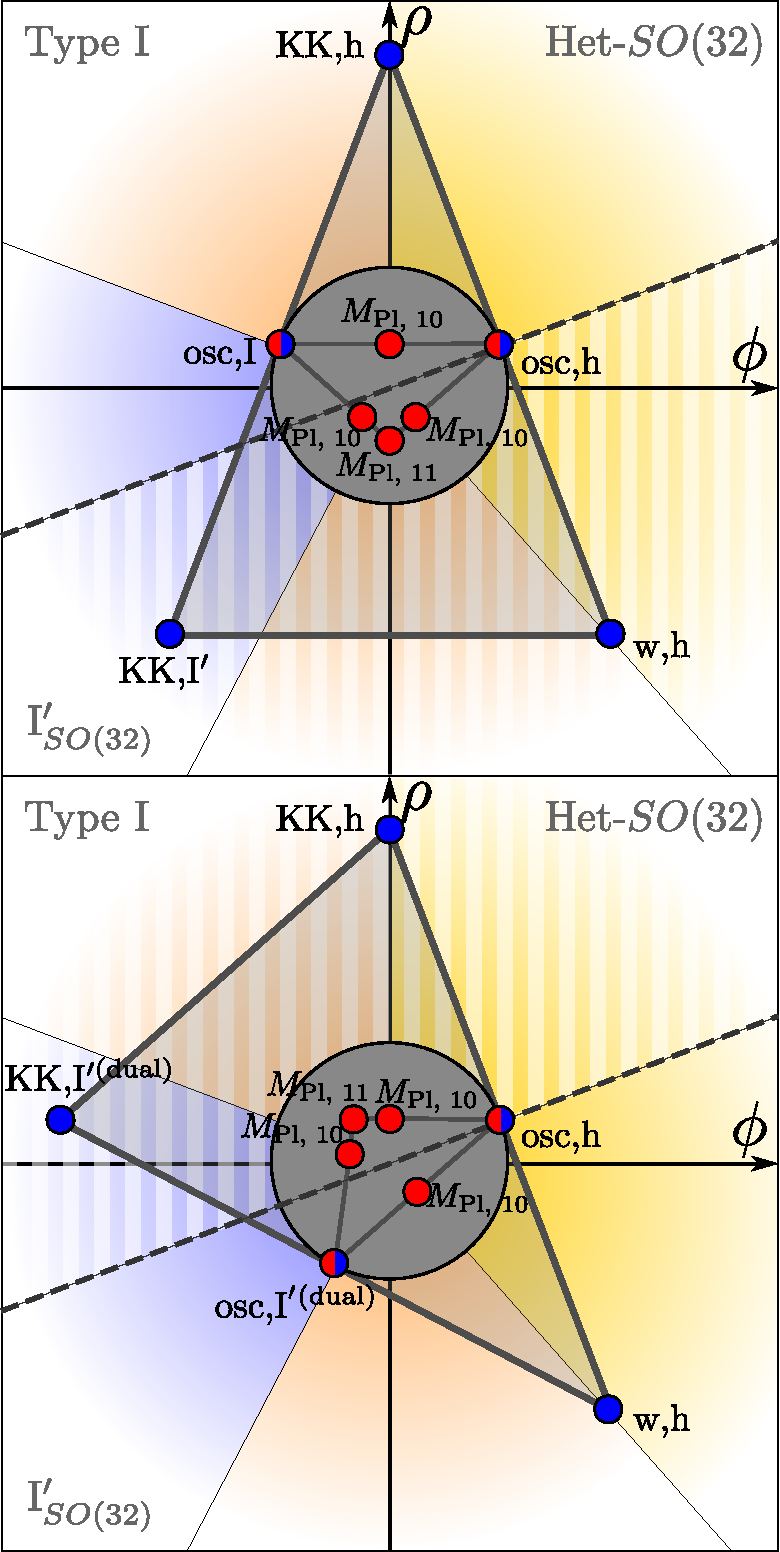
\includegraphics[width=0.4\textwidth]{so32.pdf}\label{sfig:so32}
		}
        \quad
	\subfigure[]{
			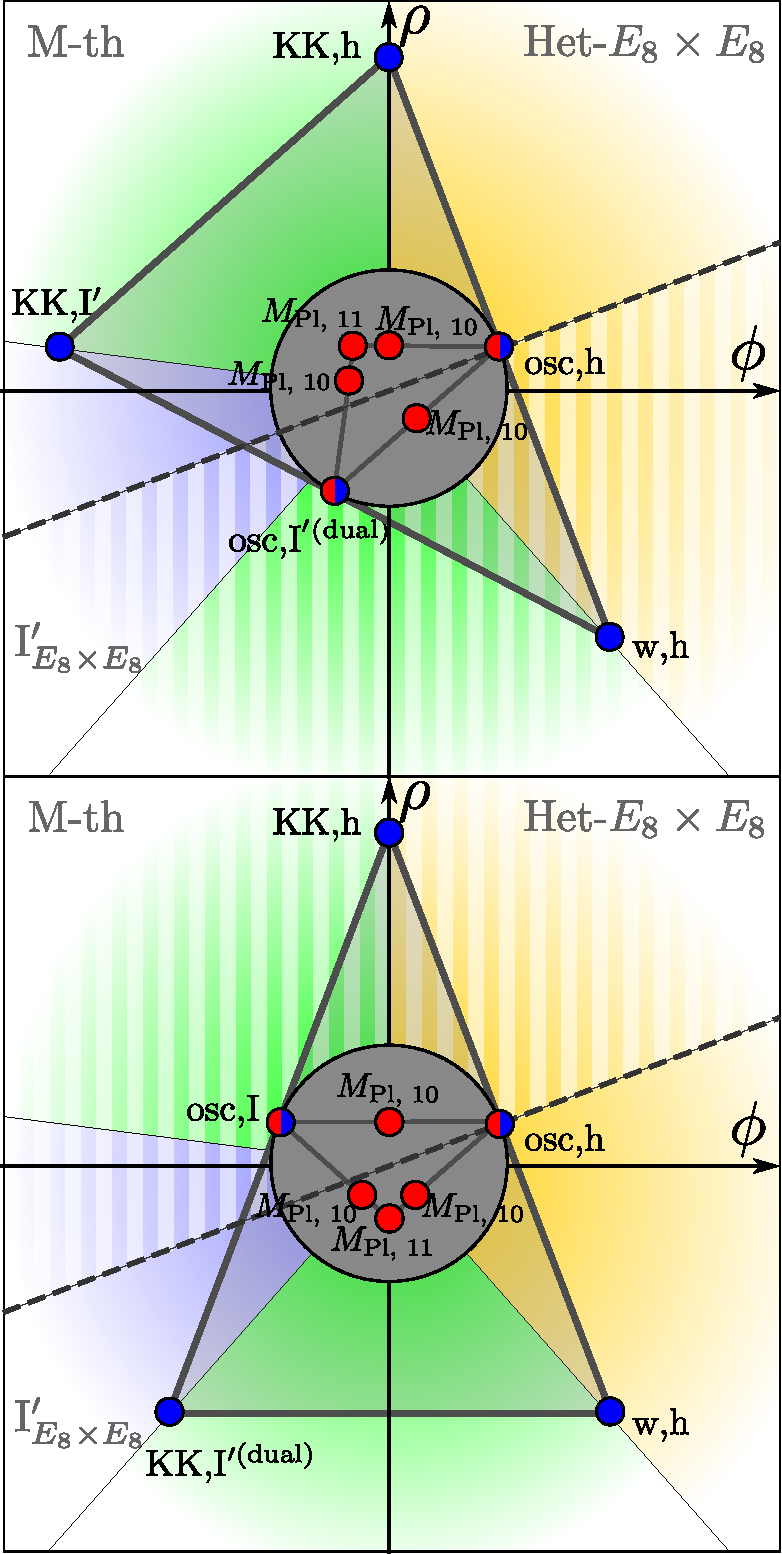
\includegraphics[width=0.4\textwidth]{e8e8.pdf}\label{sfig:e8e8}
		}
	\caption{\small Scalar charge-to-mass vectors for the towers (blue) and species scales (red) observed for the \textbf{(a)} $\mathsf{SO(32)}$ and \textbf{(b)} $\mathsf{E_8\times E_8}$ slices of the moduli space of the Heterotic string on $\mathbf{S}^1$, depending on whether the infinite distance limits (along the \emph{non}-dashed regions) are above or below the self-dual line (dashed), following the convention for the canonically normalized moduli as in \cite{Etheredge:2023odp}.}\label{fig:hets1}
\end{center}
\end{figure}
%%%%%%%%%%%%%%%%%%%%%%%%%%%%%%%%%%%%
The most interesting duality frame is that corresponding to Type I$'$ string theory, which is an orientifolded version of Type IIA on a circle, with two $O8^-$ planes at the endpoints of the interval and 16 D8-branes, whose location determines the gauge group (16 of then stacked on one orientifold for $\mathsf{SO(32)}$ and a symmetric pair of 8 D8-stacks for $\mathsf{E_8\times E_8}$), with the dilaton running between the $O8^-$ planes and the branes \cite{Polchinski:1995df}. As a result, %along some infinite distance limits (specifically those in this region with $\hat{T}$ parallel to the self-dual line)
the large radius limit of Type I$'$ leads to decompactification to a running solution of massive Type IIA in 10 dimensions (rather than a higher dimensional vacuum). This makes the scalar charge-to-mass vector of the Type I$'$ KK tower (which is non-BPS) to change non-trivially as we move in moduli space. The main result of \cite{Etheredge:2023odp} shows that warping effects make this vector to \emph{slide} in a perpendicular fashion as we move along a trajectory parallel to self-dual line and change the distance to the latter, see Figure \ref{fig:sliding}. As a function of the asymptotic direction, though, it is simply seen as a \emph{jumping} of the KK vector from one unwarped value to the other as we cross the self-dual line. (Notice that the jump occurs in opposite directions for the $\mathsf{SO(32)}$ or $\mathsf{E_8\times E_8}$ theories.) This implies that, for each duality frame, the location of the $\zeta$-vectors of the towers is the same as in the moduli space of 9d maximal supergravity --- i.e. with 32 supercharges, which becomes clear upon comparing Figure \ref{fig:hets1} with Figure \ref{fig:T2SDC&SSDC} of Section \ref{ss:9d}. The lower level of supersymmetry plays only an important role when determining how to `glue' the different patches altogether, which occurs in a very non-trivial way.
	
Hence, as long as we do not move parallel to the self-dual line in the Type I$'$ region, the relation \eqref{eq:pattern} is still satisfied, since the distribution of the towers and the species vectors is locally the same as in maximal supergravity. Each region will be characterized by a different realization of the species scale (either the 10d string scale or the 11d Planck scale), such that the convex hulls of the towers and species scale are dual to each other and the pattern is thus realized. The tower vectors were already described in \cite{Etheredge:2023odp}, so we are simply computing the species vectors as well here in order to represent everything together in Figure \ref{fig:hets1} above.
	
It remains to be seen, though, whether the pattern will also hold if moving parallel to the self-dual line in the Type I$'$ region. As explained, this limit decompactifies to a running solution in massive Type IIA with a non-trivial spatial dependence of the dilaton. In particular, this changes the exponential rate of the KK tower in comparison to the unwarped result \eqref{eq:zeta&speciesveconemodulus}, as computed in \cite{Etheredge:2023odp}.  For the $\mathsf{E_8\times E_8}$ slice\footnote{The $\mathsf{SO(32)}$ is analogous but with slightly more cumbersome expressions, see Section 3 in \cite{Etheredge:2023odp}.} one has
\begin{equation}\label{eq: sliding}
	\frac{m_{\rm KK,\, I'}}{M_{\rm Pl;\, 9}}\sim e^{-\frac{5}{2\sqrt{7}}\phi_C+\frac{3}{2}\phi_B}(1+3e^{2\phi_B})^{-1}\Longrightarrow \vec{\zeta}_{\rm KK,\, I'}=\left(\frac{1}{2}-\frac{2}{1+3e^{2\phi_B}},\frac{5}{2\sqrt{7}}\right)
\end{equation}
which is written in a basis of flat coordinates $\{\phi_B,\phi_C\}$.\footnote{This amounts to a clockwise $\frac{\pi }{2}+\arctan\left(\frac{1}{\sqrt{7}}\right)$ rotation from the $\{\phi,\rho\}$ coordinates shown in Figure \ref{fig:hets1}.} Each of these coordinates measures, respectively, the moduli space distance perpendicular and parallel to the self-dual line in the Type I$'$ frame. As already mentioned, this implies that the Type I$'$ KK modes move orthogonal to the self-dual line as a function of $\phi_B$, see Figure \ref{fig:sliding}.
%%%%%%%%%%%%%%%%%%%%%%%%%%
\begin{figure}[htb]
\begin{center}
	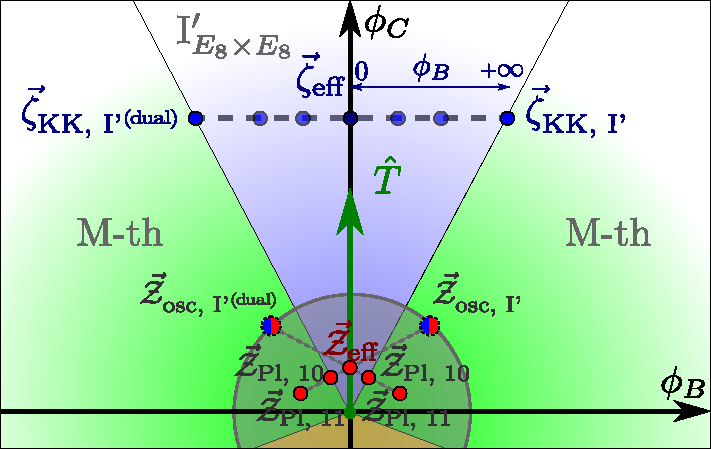
\includegraphics[scale=0.8]{sliding.pdf}
	\caption{\small Details of the $\mathsf{E_8\times E_8}$ slice of $\mathcal{M}_{\rm het}$, parameterized in terms of $\{\phi_B,\phi_C \}$. When moving with $\hat{T}=(0,1)$, thus parallel to the self-dual line, the Type I$'$ KK tower (and its dual) has a scalar charge-to-mass vector $\vec{\zeta}_{\rm KK,\; I'}$ whose expression depends on the distance $\phi_B$ of the trajectory to the self-dual line (c.f. eq. \eqref{eq: sliding}), coalescing for $\phi_B\to 0$ to $(0,\frac{5}{2\sqrt{7}})$. The fixed $\vec{\mathcal{Z}}_{\rm eff}=\left(0,\frac{2}{5\sqrt{7}} \right)$ vector satisfying the pattern is also depicted. Additional $\mathcal{Z}$-vectors associated to the obstructed emergent string towers as well as the heavier Planck masses are also presented. The $\mathsf{SO(32)}$ slice has an analogous behavior, with $\vec{\zeta}_{\rm KK,\;I'}$ located on the other side of the self-dual line, see \cite{Etheredge:2023odp}.} 
\label{fig:sliding}
\end{center}
\end{figure}
%%%%%%%%%%%%%%%%%%%%%%%%%%
At each side of the self-dual line (i.e. in each of the Type I$'$ frames) we seem to have a different tower of KK states, whose scalar charge-to-mass ratio coincides when moving exactly along the interface. We expect that these towers actually correspond to different sets of states that are mapped to each other upon performing the duality. If that is the case, they should both contribute to $\LSP$, yielding a lower value for the species cut-off (i.e. a larger value of the exponential rate) than what each tower alone would provide. The Type I$'$ string oscillator modes, though, are not expected to contribute since the string perturbative limit is obstructed. Computing this species scale from top-down string theory would constitute a project on its own, so we leave it for future work. Here, we will simply determine what should be the value for $\LSP$ along the self-dual line such that the pattern holds even for these decompactifications to running solutions. We hope that this can be useful to elucidate the fate of the pattern in these special cases.
	
Along the self-dual line, the scalar charge-to-mass vector of the KK towers is given by $\vec{\zeta}_{\rm eff}=\left(0,\frac{5}{2\sqrt{7}}\right)$, with an associated species vector $\vec{\mathcal{Z}}_{\rm eff}$ that should also point towards this direction. For decompactification limits, the species scale can be computed in terms of an \emph{effective tower} $m_{\text{eff},\, n}\sim n^{1/p_{\rm eff}}m_{\rm eff,\, 0}$ with  $p_{\rm eff}=\sum_i p_i$ and $m_{i,\, n}\sim n^{1/p_{i}}m_{i,\, 0}$, see Section \ref{ss:MultipleTowers} for details on this. We do not expect $p_{\rm eff}=1$ since this would correspond to having a single KK tower decompactifying one dimension, nor $p_{\rm eff}=2$ since it would rather indicate a double decompactification. In fact, for the pattern to hold, one can check that the required value for the density parameter is somewhat in between, namely $p_{\rm eff}=\frac{4}{3}$, which can be obtained upon identifying
%
\begin{equation}
	\frac{\Lambda_{\rm eff}}{M_{\text{Pl;}\, 9}}=\left(\frac{m_{\rm eff}}{M_{\text{Pl;}\, 9}}\right)^{\frac{p_{\rm eff}}{9-2+p_{\rm eff}}}=e^{-\frac{2}{5\sqrt{7}}\phi_C}\Longrightarrow \vec{\mathcal{Z}}_{\rm eff}=\left(0,\frac{2}{5\sqrt{7}} \right)\, .
\end{equation}
%
This value would imply $\vec{\zeta}_{\rm eff}\cdot\vec{\mathcal{Z}}_{\rm eff}=\vec{\zeta}_{\rm KK,\, I'}\cdot\vec{\mathcal{Z}}_{\rm eff}=\vec{\zeta}_{\rm KK,\, I'^{\,(dual)}}\cdot\vec{\mathcal{Z}}_{\rm eff}=\frac{1}{7}$, satisfying the pattern for any $\phi_B\geq 0$. Along the self-dual line, the Type I$'$ radion --- measured in 10d Planck units --- and string coupling scale as $R_{\rm I'}M_{\rm Pl; 10}=g_{\rm I'}^{-5/4}\sim e^{\frac{5\sqrt{7}}{16}\phi_C}$. This implies that the species cut-off should scale as $\frac{\LSP}{M_{\rm Pl;\, 10}}\sim (R_{\rm I'}M_{\rm Pl;\, 10})^{-\frac{32}{175}}\sim g_{\rm I'}^{\frac{8}{35}}$, although it is not possible for us to elucidate the separate dependence on the radion and the dilaton. It would be interesting to check, directly from string theory, whether this behaviour of the species scale is indeed realized and the structure of the KK towers (taking into account the large warping associated to decompactifying to a running solution) is such that effectively implies  $p_{\rm eff}=\frac{4}{3}$. Hence, whether the pattern is fulfilled in this particular asymptotic direction remains open and is left for future investigation. Similarly, it is easy to see that with these state of affairs the bound \eqref{eq:lowerboundspecies} introduced in Chapter \ref{ch:bounds} would be equally satisfied along every possible infinite distance direction, including those parallel to the self-dual line. 
	
%In these cases it is not at all clear which quantity should be taken as the species scale, so we are not able to check the $\vec{\zeta}_{\rm t}\cdot\vec{\mathcal{Z}}_{\rm sp}=\frac{1}{d-2}$ pattern along this particular direction.
	
%However, for any other choice of asymptotic limit, the different towers remain fixed, with their distribution at any side corresponding to that of maximal supergravity in 9d, see Section \ref{ss:9d} and Figures \ref{fig:T2SDC&SSDC} and \ref{fig:hets1}. The species scale on the different limits will be given by the expected upper-dimensonal Planck/string masses, such that the convex hulls of the towers and species scale are dual to each other and the pattern is thus realized.
	
%As described in \cite{Etheredge:2023odp}, other slices \cite{Aharony:2007du, Montero:2022vva} of the full moduli space either feature fixed towers and species, such as in maximal supergravity in 9d, or the same sliding described in the previous examples. In any event, this results in the \eqref{eq:pattern} pattern being realized in an ample variety of limits in 9d with 16 supercharges, with the possible caveat of trajectories parallel to the self-dual line, which decompactify to a running solution, where the exact nature of the species scale is not yet understood. \fixme{IR: Algo más?}
	
	
	
\subsection{M-theory in 7d}\label{ss:Mthy7dpattern}
	
Let us now turn to our second example and consider M-theory compactified on a $K3$ surface, leading to a supersymmetric set-up in 7d with 16 supercharges as well. This setting exhibits many features that will be explained in more detail when discussing 4d theories arising from Calabi--Yau compactifications. Furthermore, our analysis here nicely complements the work performed in \cite{Lee:2019xtm}, where the emphasis was placed on the leading tower of states rather than the species scale. Here we will focus again on \emph{attractive} $K3$ two-folds, since in that case all relevant moduli dependence arises just from the K\"ahler sector.

To check the pattern in the present context, we need to know the explicit form of the moduli space metric, which is captured as usual by the kinetic terms in the scalar lagrangian. The full bosonic action was already discussed in Section \ref{sss:MtheoryonK3}, so we will refer oftentimes to the material presented there. Thus, in the attractive case, the relevant line element reads
%
\begin{equation}\label{eq:7dMthymetric}
	\begin{aligned}
		ds_{\rm VM}^2\, = \, \frac{9}{20} d\mathcal{V}_{K3}^2 + \mathsf{G}_{a b}\, d\tilde{t}^a d \tilde{t}^b\, ,
	\end{aligned}
\end{equation}
%
where $\mathcal{V}_{K3}$ denotes the overall internal volume and $\{ \tilde{t}^a\}$ are constrained K\"ahler moduli, see discussion around eq. \eqref{eq:7dMthyattractive}. The latter describe a (classically exact) subspace of the group coset \eqref{eq:cosetspace7d}, which admits a natural metric given by
%
\begin{equation}\label{eq:7dmodspacemetricpattern}
	\begin{aligned}
		\mathsf{G}_{a b} = \frac{t_a t_b}{\mathcal{V}_{K3}}- \eta_{a b} = \tilde{t}_a \tilde{t}_b -\eta_{a b}\, ,
	\end{aligned}
\end{equation}
%
where the indices are lowered with the intersection form $\eta_{a b}$. 
	
Regarding the infinite distance boundaries of such moduli space, there are several of them, according to which moduli are sent to infinity: the large volume point, the small `radius' limit, a \emph{unique} type of infinite distance degeneration at constant $\mathcal{V}_{K3}$ and combinations thereof. We discuss each of them in turn.
	
\subsubsection*{The large/small volume limits}
	
Let us start with the large volume singularity $\mathcal{V}_{K3} \to \infty$, which of course lies at infinite distance in the field space metric defined from eq. \eqref{eq:7dMthymetric} above. It corresponds to the full decompactification limit, where the $K3$ manifold grows large and we come back effectively to 11d supergravity. Thus, the infinite tower of asymptotically light states is given by the KK tower, whose mass is given by
%
\begin{equation}
	\frac{m_{\text{KK, K3}}}{M_{\text{Pl};\, 7}} = \mathcal{V}_{K3}^{-9/20} \quad \Longrightarrow \quad \vec{\zeta}_{\text{KK, K3}} = \left( \frac{9}{20} \frac{1}{\mathcal{V}_{K3}}, 0, \ldots, 0 \right)\, ,
\end{equation}
%
where we have used that the 7d and 11d Planck scales are related by $M_{\text{Pl};\, 7}^5= M_{\text{Pl};\, 11}^5 \mathcal{V}_{K3}$. The associated species scale corresponds to the 11d Planck mass, such that upon taking the inner product between $\vec{\zeta}_{\text{KK, K3}}$ and $\vec{\mathcal{Z}}_{\text{sp}} = \frac{4}{9} \vec{\zeta}_{\text{KK, K3}}$ (c.f. eq. \eqref{eq:eff-vector}) we find that $\vec{\zeta}_{\text{KK, K3}} \cdot \vec{\mathcal{Z}}_{\text{sp}}= \frac{1}{5}$, in agreement with \eqref{eq:pattern}.
	
The small `radius' limit, namely $\mathcal{V}_{K3} \to 0$, is of different physical nature. One can argue that it corresponds to an emergent string limit, where an asymptotically tensionless and weakly coupled Heterotic string emerges at infinite distance. Indeed, it is possible to construct an Heterotic-like string by wrapping the M5-brane on the whole $K3$ surface \cite{Cherkis:1997bx,Park_2009}, with a tension in 7d Planck units which reads as follows
%
\begin{equation}
	\frac{T_{\text{M5}}}{M_{\text{Pl};\, 7}^2} = \mathcal{V}_{K3}^{3/5} \quad \Longrightarrow \quad \vec{\zeta}_{\text{osc, M5}} = \left( -\frac{3}{10} \frac{1}{\mathcal{V}_{K3}}, 0, \ldots, 0 \right)\, .
\end{equation}
%
Moreover, there are additional $\frac{1}{2}$-BPS states arising from wrapped M2-branes on certain holomorphic curves within the $K3$, which correspond to perturbative winding modes of the dual Heterotic string on $\mathbf{T}^3$.\footnote{Note that since $H^2(K3, \mathbb{Z})$ defines a lattice of signature $(3,19)$ there are precisely 3 non-equivalent holomorphic curve classes with non-negative self-intersection, and thus non-contractible. These should correspond to the 3 winding modes sectors of the dual Heterotic string on $\mathbf{T}^3$.} Their mass operator can be deduced from the DBI action (c.f. eq. \eqref{eq:DBICSactionMpbranes}), and yields 
%
\begin{equation}\label{eq:M2mass&vectors}
	\frac{m_{\text{M2}}^{(a)}}{M_{\text{Pl};\, 7}} = t^a\, \mathcal{V}_{K3}^{-1/5} = \tilde{t}^a\, \mathcal{V}_{K3}^{3/10} \quad \Longrightarrow \quad \vec{\zeta}^{\,(a)}_{\text{M2}} = \left( -\frac{3}{10} \frac{1}{\mathcal{V}_{K3}}, 0, \ldots, -\frac{1}{\tilde{t}^a}, \ldots, 0 \right)\, ,
\end{equation}
%
where the non-zero entries correspond to the overall volume component and the one associated to the rescaled $\tilde{t}^a$ modulus (see discussion after eq. \eqref{eq:7dMthymetric}). It is therefore clear that upon contracting $\vec{\zeta}_{\text{t}}= \lbrace \vec{\zeta}_{\text{osc, NS5}}, \vec{\zeta}^{\,(a)}_{\text{M2}} \rbrace$ with $\vec{\mathcal{Z}}_{\text{sp}}=\vec{\zeta}_{\text{osc, NS5}}$, one obtains $\vec{\zeta}_{\text{t}} \cdot \vec{\mathcal{Z}}_{\text{sp}}= \frac{1}{5}$, thus fulfilling the pattern.
	
\subsubsection*{Infinite distance at fixed (overall) volume}
	
Let us consider now infinite distance limits with the overall volume kept fixed and constant. In fact, as demonstrated in \cite{Lee:2019xtm} (see also earlier related works in \cite{Lee:2018urn,Lee:2018spm}), for such a limit to exist it must be possible to select some $\omega_0 =\sum_a c^a \omega_a \in H^{1,1}(X_3,\mathbb{Z})$ (with $c^a \geq 0$) such that\footnote{The fact that the limit \eqref{eq:T2limit7d} lies at infinite distance with respect to the metric \eqref{eq:7dmodspacemetricpattern} follows from the asymptotic dependence of $\mathsf{G}_{a b}$:
\begin{equation}
	\notag \Delta= \int_1^{\infty} \dd \sigma \sqrt{\mathsf{G}_{a b} \frac{d \tilde{t}^a}{d \sigma} \frac{d \tilde{t}^b}{d \sigma}}\, \sim\, \int_1^{\infty} \dd \log \left(\tilde{t}^0 \right)\, \to\, \infty\, ,
\end{equation}
where we have used that $\mathsf{G}_{i j}=\eta_{0i} \eta_{0j} \left( \tilde{t}^0\right)^2 + \mathcal{O} (\sigma^0)$, $\mathsf{G}_{0 j}=\eta_{0j} \eta_{i 0} \tilde{t}^j \tilde{t}^0 - \eta_{0i} + \mathcal{O} (1/\sigma^2)$ and $\mathsf{G}_{0 0}= \eta_{0j} \eta_{i 0} \tilde{t}^i \tilde{t}^j$.}
%
\begin{equation}\label{eq:T2limit7d}
	J= t^0 \omega_0 + t^i \omega_i %= \sigma\, \omega_0 + \frac{t^i}{\sigma}\, \omega_i
	\, , \qquad \text{with}\ \ t^0 = \sigma,\ t^i = \frac{a^i}{\sigma}, \quad \sigma \to \infty\, ,
\end{equation}
%
where $i=1, \ldots, 19,$ and the basis $\lbrace \omega_0, \omega_i\rbrace$ verifies that $\omega_0 \cdot \omega_0=0$ and $\sum_i a^i\, \omega_0 \cdot \omega_i= \mathcal{V}_{K3} + \mathcal{O}(1/\sigma^2)$. Geometrically, the very existence of such a limit enforces the attractive $K3$ to admit some elliptic fibration over a $\mathbb{P}^1$-base, with the genus-one fibre $\mathcal{C}_0$ being Poincaré dual to the K\"ahler cone generator $\omega_0$. Such holomorphic curve shrinks upon taking the limit \eqref{eq:T2limit7d}, whilst the base grows at the same rate so as to keep the overall $\mathcal{V}_{K3}$ fixed and finite.
	
Given the behavior of the different 2-cycles along the limit \eqref{eq:T2limit7d}, there exist potentially two kinds of infinite towers of states. First, there are the supergravity KK modes associated to the $\mathbb{P}^1$-base, whose volume grows asymptotically. The mass scale of such tower behaves as follows
%
\begin{equation}\label{eq:massP1}
	\frac{m_{\text{KK},\, \mathbb{P}^1}}{M_{\text{Pl};\, 7}}=\frac{1}{\left(\tilde{t}^0\right)^{1/2}\, \mathcal{V}_{K3}^{9/20}} \quad \Longrightarrow \quad \vec{\zeta}_{\text{KK},\, \mathbb{P}^1} = \left(\frac{9}{20} \frac{1}{\mathcal{V}_{K3}}, \frac{1}{2 \tilde{t}^0}, 0, \ldots, 0 \right)\, ,
\end{equation}
% 
so that it becomes (exponentially) light upon probing the $\tilde{t}^0 \to \infty$ limit. In addition, there is a second infinite set of states becoming light even faster, which arise from M2-branes wrapping the genus-one fibre. Their mass is controlled by the volume of the latter
%
\begin{equation}\label{eq:M2massFthy}
	\frac{m_{\text{M2}}}{M_{\text{Pl};\, 7}} = \mathcal{V}_{\mathcal{C}_0}\, \mathcal{V}_{K3}^{-1/5}=\frac{\mathcal{V}_{K3}^{3/10}}{\tilde{t}^0} \quad \Longrightarrow \quad \vec{\zeta}_{\text{M2}} = \left( -\frac{3}{10} \frac{1}{\mathcal{V}_{K3}}, \frac{1}{\tilde{t}^0}, 0, \ldots, 0 \right)\, ,
\end{equation}
%    
and they can be seen to correspond to the dual KK replica implementing the duality between M-theory on $K3$ and F-theory on $K3\times \mathbf{S}^1$ \cite{Vafa:1996xn,Lee:2019xtm}. However, in order to correctly interpret what is the resolution of the singularity in QG, we need to study the behavior of the species scale. One can thus associate two such scales, one for each tower, as follows (c.f. eq. \eqref{eq:eff-vector})
%
\begin{align}\label{eq:species7d}
	\notag \frac{\Lambda_{\rm M2}}{M_{\text{Pl};\, 7}} &\simeq \left(m_{\text{M2}}\right)^{1/6} = \frac{\mathcal{V}_{K3}^{1/20}}{\left( \tilde{t}^0\right)^{1/6}}\quad \Longrightarrow \quad \vec{\mathcal{Z}}_{\text{Pl},\, 8} = \left( -\frac{1}{20} \frac{1}{\mathcal{V}_{K3}}, \frac{1}{6\, \tilde{t}^0}, 0,\ldots, 0 \right)\, ,\\
	\frac{\Lambda_{\text{Pl},\, 9}}{M_{\text{Pl};\, 7}} &\simeq \left(m_{\text{KK},\, \mathbb{P}^1}\right)^{2/7} = \frac{1}{\left(\tilde{t}^0\right)^{1/7}\, \mathcal{V}_{K3}^{9/70}} \quad \Longrightarrow \quad \vec{\mathcal{Z}}_{\text{Pl},\, 9} = \left(\frac{9}{70} \frac{1}{\mathcal{V}_{K3}}, \frac{1}{7 \tilde{t}^0}, 0, \ldots, 0 \right)\, , 
\end{align}
%
which coincide with the 8d Planck scale\footnote{This can be easily checked upon identifying $R_8 = \frac{(\tilde{t}^0)^{5/6}}{\mathcal{V}_{K3}^{1/4}}$, where $R_8$ denotes the radius (in 8d Planck units) of the F-theory circle, as well as the relation between the 8d and 7d Planck scales, namely $M_{\text{Pl};\, 7}^5= M_{\text{Pl};\, 8}^5 2\pi R_8$.} (in the F-theory frame) and the 9d Planck scale, respectively. We are not done yet though, since both sets of states can be combined together forming bound states, namely the wrapped M2-branes may have non-trivial momentum along the $\mathbb{P}^1$-base. Furthermore, such `mixed' states contribute to the computation of a third candidate for the species scale, whose $\mathcal{Z}$-vector reads (see eq. \eqref{eq:effectiveKKspeciesvector})
%
\begin{align}\label{eq:speciesKK10d}
	\vec{\mathcal{Z}}_{\text{Pl},\, 10} = \frac{1}{8} \left( \vec{\zeta}_{\text{M2}} + 2 \vec{\zeta}_{\text{KK},\, \mathbb{P}^1}\right) = \left(\frac{3}{40} \frac{1}{\mathcal{V}_{K3}}, \frac{1}{4 \tilde{t}^0}, 0, \ldots, 0 \right)\, , 
\end{align}
%
thus signalling towards decompactification to 10d Type IIB string theory. In Figure \ref{fig:CHMthy7d} all these vectors are plotted --- both for the mass and species scale, including those relevant in the large/small $K3$ volume limit, as previously discussed. 
	
With this, we are now ready to check what is the minimum $\LSP$ dominating the asymptotic physics along the limit \eqref{eq:T2limit7d}. Indeed, it is easy to see either from the formulae above or the diagram in Figure \ref{fig:CHMthy7d}, that this becomes the 10d Planck scale. Therefore, such limit may be interpreted as some `nested' decompactification, first from 7d M-theory to 8d F-theory (as remarked in \cite{Lee:2019xtm}) and then up to ten dimensions, effectively sending all supersymmetry breaking defects (i.e. D7-branes and $O7$-planes) to infinity and restoring maximal chiral supergravity in 10d. Hence, a quick computation reveals that the pattern $\vec{\zeta}_{\text{M2}} \cdot \vec{\mathcal{Z}}_{\text{Pl},\, 10}= \frac{1}{5}$ is also verified in this limit (to leading order in $1/\tilde{t}^0$). 
	
%%%%%%%%%%%%
\begin{figure}[htb]
	\begin{center}
		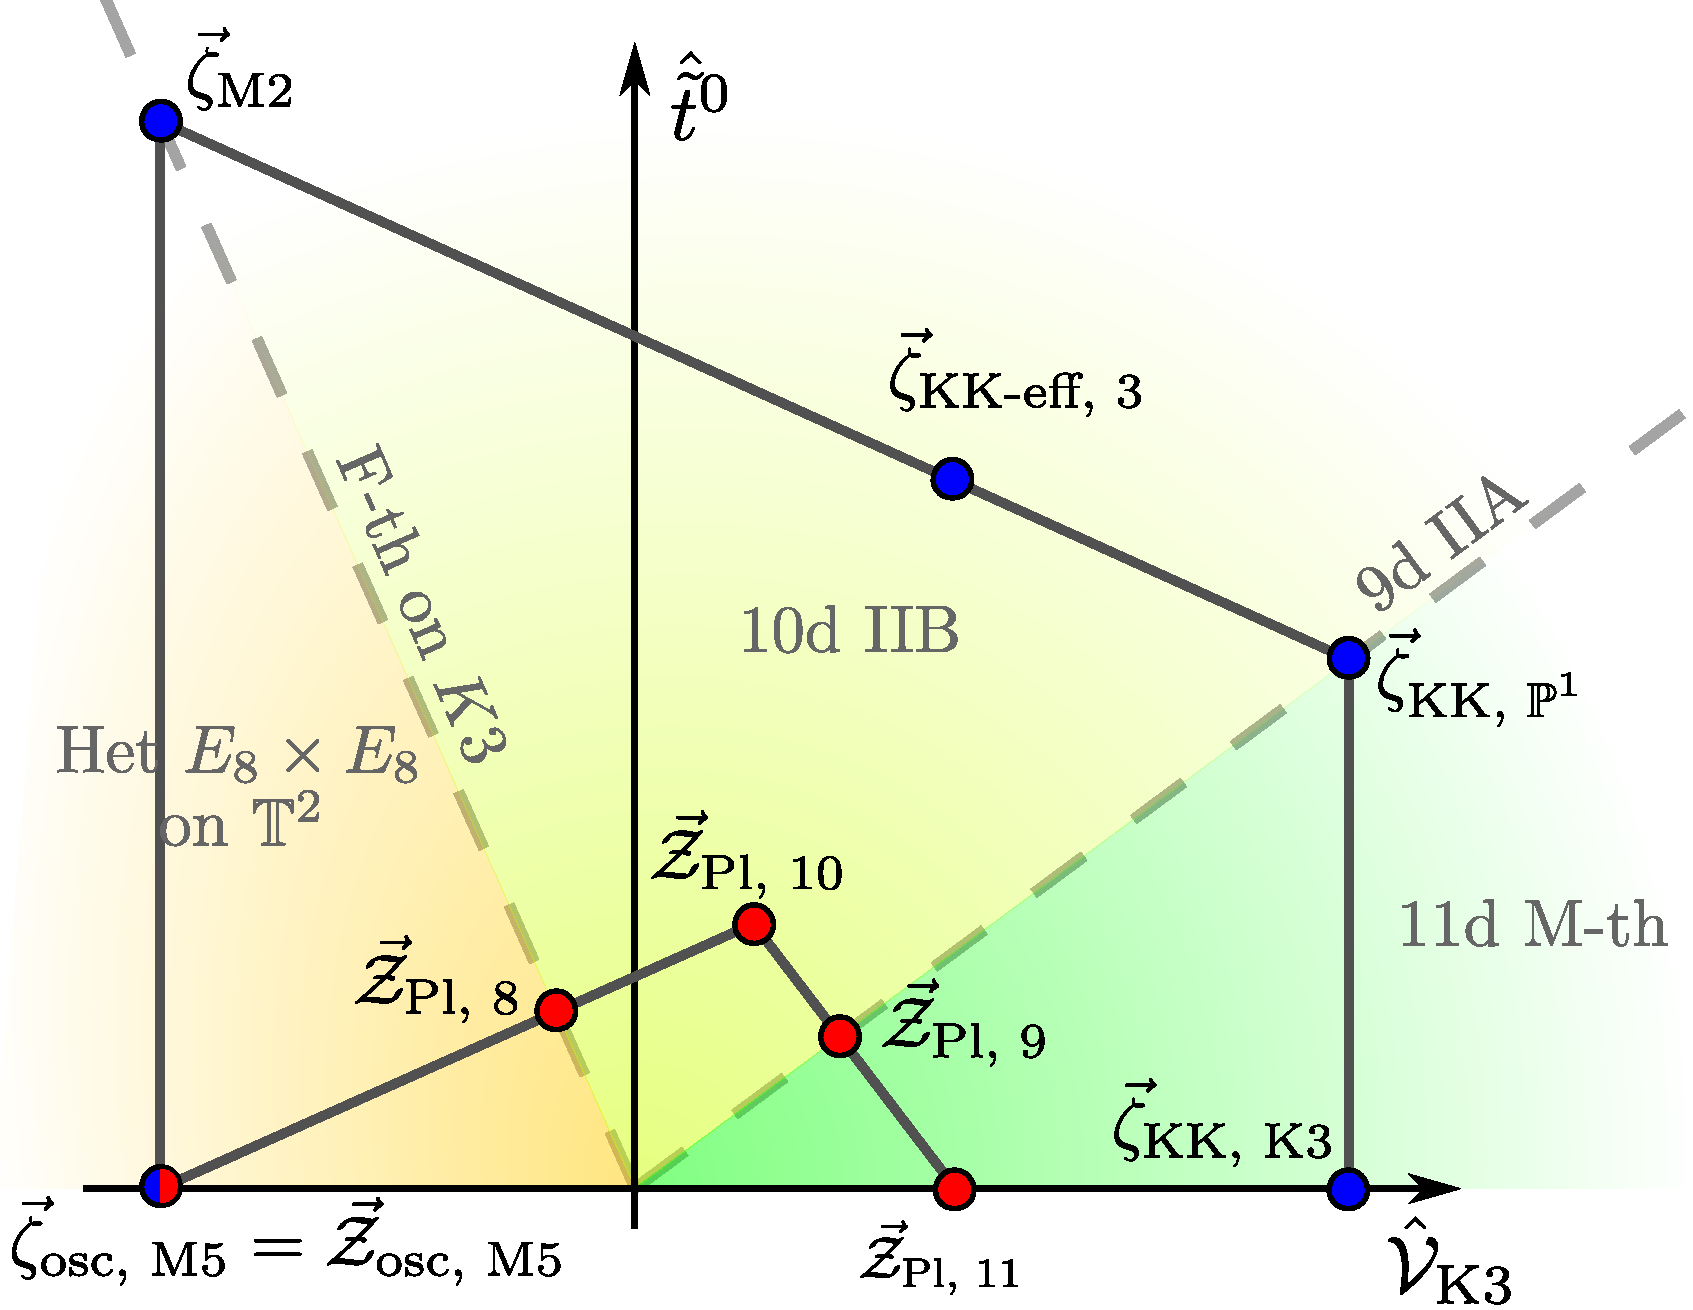
\includegraphics[scale=.35]{Mth_K3.pdf}
		\caption{\small Convex hulls for the lightest towers (blue) and species scale (red) in M-theory compactified on an attractive $K3$ surface, using a flat frame $\lbrace \hat{\tilde{t}}^0, \hat{\mathcal{V}}_{K3}\rbrace$, in which the equations of the different vectors are $\vec{\zeta}_{\rm osc,\; M5}=\vec{\mathcal{Z}}_{\rm osc,\; M5}=\left(-\frac{1}{\sqrt{5}},0\right)$, $\vec{\zeta}_{\rm M2}=\left(-\frac{1}{\sqrt{5}},1\right)$, $\vec{\zeta}_{\rm KK-eff,\; 3}=\left(\frac{2}{3\sqrt{5}},\frac{2}{3}\right)$, $\vec{\zeta}_{{\rm KK},\; \mathbb{P}^1}=\left(\frac{3}{2\sqrt{5}},\frac{1}{2}\right)$, $\vec{\zeta}_{{\rm KK},\; K3}=\left(\frac{3}{2\sqrt{5}},0\right)$, $\vec{\mathcal{Z}}_{\rm Pl,\; 8}=\left(-\frac{1}{6\sqrt{5}},\frac{1}{6}\right)$, $\vec{\mathcal{Z}}_{\rm Pl,\; 10}=\left(\frac{1}{4\sqrt{5}},\frac{1}{4}\right)$, $\vec{\mathcal{Z}}_{\rm Pl,\; 9}=\left(\frac{3}{7\sqrt{5}},\frac{1}{7}\right)$ and $\vec{\mathcal{Z}}_{\rm Pl,\; 11}=\left(\frac{2}{3\sqrt{5}},0\right)$. It is easy to see that both polytopes are dual to each other (with respect to the 1-sphere of radius $\frac{1}{\sqrt{d-2}}=\frac{1}{\sqrt{5}}$), and thus the pattern is satisfied. The different limiting theories, which can be deduced by looking at the dominant species scale in each region of the moduli space, are also shown for completeness.} 
		\label{fig:CHMthy7d}
	\end{center}
\end{figure}
%%%%%%%%%%%%
	
\subsubsection*{Intermediate limits}
	
To conclude, let us briefly comment on the possibility of superimposing any of the previous limits, thus sending both the overall $K3$ volume and the $\tilde{t}^0$ K\"ahler modulus to infinity at different rates, a priori. In fact, upon comparing the different species scale that can arise (and even compete) at distinct corners of the moduli space, one can indeed separate these asymptotic regions into different sectors, depending on which specific scale dominates (see Figure \ref{fig:CHMthy7d}). In any event, it is straightforward to verify that the pattern is respected in all such cases, due to the non-trivial gluing conditions between the different patches.

\section{Examples in 4d $\mathcal{N}=2$ EFTs}
\label{s:8supercharges}
	
We now turn to theories with 8 supercharges. In particular, we will focus on 4d $\mathcal{N}=2$ set-ups arising upon compactifying Type II string theory on Calabi--Yau three-folds. The singularity structure of the moduli space of these theories is very rich and has been thoroughly studied in the literature, providing for different types of infinite distance limits. In Sections \ref{ss:preliminary}-\ref{ss:commentsTypeIIB} we discuss the vector multiplet sector by studying different concrete examples as well as presenting general arguments in favour of satisfying the pattern. Section \ref{ss:hypers} analyzes the effect of (towers of) instanton corrections on singularities located classically at infinite distance, which are nevertheless excised and deflected within the true quantum hypermultiplet moduli space.
	
\subsection{The vector multiplet moduli space}
\label{ss:preliminary}
	
Recall from Section \ref{sss:4dN=2basics} that the moduli space of 4d $\mathcal{N}=2$ theories factorizes at the two-derivative level in two pieces: the vector multiplet and the hypermultiplet sectors. For concreteness, we focus on theories obtained upon compactifying Type IIA string theory on a Calabi--Yau three-fold $X_3$, although we will make some comments regarding the Type IIB counterpart later on in Section \ref{ss:commentsTypeIIB}.

Since we will only be interested in the computation of the relevant scalar charge-to-mass vectors as well as the corresponding species scale, we restrict ourselves to the scalar and gravitational sectors of the 4d action \eqref{eq:IIAaction4d}, effectively forgetting about the vector fields. Thus, in the low energy regime, the relevant piece of the action reads
%
\begin{equation}\label{eq:IIAscalaraction4d}
	\begin{aligned}
		\ S^{\text{4d}}_{\rm IIA}\, \supset\, & \frac{1}{2\kappa^2_4} \int \mathcal{R} \star 1 -2 G_{a\bar b}\, d z^a\wedge \star d\bar z^b + 2h_{pq}\, d q^p \wedge \star d q^q\, ,
	\end{aligned}
\end{equation}
%
where the fields $z^a=b^a+{\rm i}t^a$, $a=1,\ldots, h^{1,1}$, describe the (complexified) K\"ahler sector of the theory, whereas the scalars in the various hypermultiplets (including e.g., the complex structure moduli) are denoted by $q^p$. In the following, we will particularize to the vector multiplet moduli space, leaving the analysis of the hypermultiplet sector for Section \ref{ss:hypers}. 

The explicit expression for metric associated to the complex fields $\{ z^a \}$ is (c.f. eq. \eqref{eq:kahlersectormetric})
%
\beq\label{eq:kahlersectormetricpattern}
	G_{a\bar b}=\partial_a \partial_{\bar{b}} K_{\text{ks}}= -\partial_a \partial_{\bar{b}} \log \left( 8 \mathcal{V}_{X_3} \right)\, ,
\eeq
%
where $\mathcal{V}_{X_3}$ is the classical volume of the three-fold measured in string units. By Mirror Symmetry, this effective theory can be equivalently described as arising from compactifying Type IIB on the mirror Calabi--Yau, such that the role of K\"ahler and complex structure moduli get exchanged (see Section \ref{ss:dualitieswithlowersusy} for details). The different types of infinite distance limits in the vector multiplet sector can then be systematically classified using the theory of Mixed Hodge Structures \cite{Grimm:2018ohb, Grimm:2018cpv}. However, in the present work, we will analyze each of these limits using the language of Type IIA compactifications, since the microscopic interpretation of the corresponding asymptotic limit (either decompactification or emergent string limit \cite{Lee:2019wij}) becomes more apparent from this point of view.
	
\subsubsection*{Classification of infinite distance limits at large volume}
\label{sss:largevolume}
	
From the perspective of Type IIA string theory, we need to particularize to the large volume patch, where one can safely ignore both $\alpha'$ and worldsheet instanton contributions which further correct the form of the metric displayed in \eqref{eq:kahlersectormetricpattern}. Still, the structure of possible infinite distance singularities is very rich as we review in what follows. Thus, according to \cite{Corvilain:2018lgw,Grimm:2018cpv,Grimm:2018ohb}, we can parametrize infinite distance limits within the K\"ahler cone in terms of trajectories of the form
%
\beq \label{eq:singlefieldlim}
	\lbrace t^i\rbrace = t^1,\ldots , t^{n}\to \infty\, ,\qquad n\leq h^{1,1}(X_3)\, ,
\eeq
%
with $b^i$ approaching finite values. The several distinct types of infinite distance limits have been thoroughly studied and classified by different means in \cite{Corvilain:2018lgw,Lee:2019wij}, and can be divided into three classes shown in Table \ref{tab:intersN=2} below, depending on the behavior of the intersection numbers $\mathcal{K}_{abc}$ with the asymptotic direction taken. More details about the notation in terms of Roman numerals can be found in \cite{Grimm:2018ohb}, whilst that in terms of $J$-class A/B can be found in \cite{Lee:2019wij} (see also \cite{Lee:2019tst}). Geometrically, these three classes correspond to different fibration structures: the \emph{unique} limit in which the overall volume of $X_3$ blows up uniformly, thus corresponding to the large volume point; the ones in which the CY$_3$ possesses an elliptic fibration over some K\"ahler two-fold; and those in which the three-fold develops either some $K3$ or $\mathbf{T}^4$ fibration over a $\mathbb{P}^1$-base. We will consider in the upcoming subsections specific examples of each representative class of limit followed by a general analysis of each singularity type, providing all of them more evidence in favour of the pattern here described. 
	
In Table \ref{tab:limitsN=2}, we summarize the microscopic interpretation of the leading tower of states becoming light at each type of infinite distance limit, as well as the physical realization of the species scale for each case. Recall that, in this section, we consider infinite distance limits lying purely within the vector multiplet moduli space, while all hypermultiplet scalars (including the 4d dilaton) remain fixed. To achieve this, we will sometimes need to co-scale properly certain ten-dimensional variables \cite{Lee:2019wij}. For instance, if we want to keep the 4d dilaton, $\varphi_4 =\phi-\frac{1}{2} \log \mathcal{V}$, fixed and \emph{finite}, one needs to rescale accordingly the 10d dilaton $\phi$, which will bring us to the strong coupling regime of Type IIA as we will see below in more detail. For other limits involving also the hypermultiplets, see Section \ref{ss:hypers}.

%%%%%%%%%%%%%%%%%%%%%%%%%%%%%%%
\begin{table}[h!!]\begin{center}
	\renewcommand{\arraystretch}{0.80}
		\begin{tabular}{|c|c|c|}
		\hline 
		Type \cite{Corvilain:2018lgw} & Type \cite{Lee:2019wij} & Intersection numbers \\
		\hline 
		\hline 
		IV$_d$ & --- & $\text{rk}(\boldsymbol{\kappa}^{(n)}) = \text{rk}(\boldsymbol{\kappa}^{(n)}_a)= 1$ and $\text{rk}(\boldsymbol{\kappa}^{(n)}_{a b})=d$   \\
		III$_c$ & $J$-class A & $\text{rk}(\boldsymbol{\kappa}^{(n)}) = 0$, $\text{rk}(\boldsymbol{\kappa}^{(n)}_a)= 1$ and $\text{rk}(\boldsymbol{\kappa}^{(n)}_{a b})=c+2$ \\
		II$_b$ & $J$-class B & $\text{rk}(\boldsymbol{\kappa}^{(n)}) = \text{rk}(\boldsymbol{\kappa}^{(n)}_a)= 0$ and $\text{rk}(\boldsymbol{\kappa}^{(n)}_{a b})=b$ \\
		\hline
	\end{tabular}
\caption{\small Infinite distance limits in the large volume regime within the vector multiplet moduli space of Type IIA compactified on a CY$_3$. They can be classified in terms of the behavior of the triple intersection numbers $\mathcal{K}_{abc}$ via Mixed Hodge Theory \cite{Corvilain:2018lgw}, or using a purely geometrical analysis \cite{Lee:2019wij}. The following notation has been introduced: $\boldsymbol{\kappa}^{(n)}_{a b} = \sum_{i=1}^n \mathcal{K}_{i a b}$, $\boldsymbol{\kappa}^{(n)}_{a} = \sum_{i,j=1}^n \mathcal{K}_{i j a}$, $\boldsymbol{\kappa}^{(n)} = \sum_{i,j,k=1}^n \mathcal{K}_{i j k}$ and $\text{rk}(\cdot)$ denotes the rank of the corresponding matrix.}
\label{tab:intersN=2}
\end{center}
\end{table}
%%%%%%%%%%%%%%%%%%%%%%%%%%%%%%%
\begin{table}[h!!]\begin{center}
\renewcommand{\arraystretch}{1.00}
	\begin{tabular}{|c|c|c|c|c|}
		\hline
		Type \cite{Corvilain:2018lgw} & Type \cite{Lee:2019wij} &  Fibration structure  &  Dominant Tower & $\LSP$\\
		\hline 
		\hline 
		IV$_d$ & --- & Unspecified  & D0 & $M_{\text{Pl};\, 5}$\\
		III$_c$  & $J$-class A & Elliptic Fibration & D0 and D2 on $\mathbf{T}^2$ & $M_{\text{Pl};\, 6}$\\
		II$_a$ & $J$-class B & $K3$ or $\mathbf{T}^4$ Fibration & NS5 on $K3/\mathbf{T}^4$ & $\sqrt{T_{\rm NS5}}$\\
		\hline
	\end{tabular}
	\caption{\small Infinite distance limit classification according to refs. \cite{Corvilain:2018lgw} and \cite{Lee:2019wij}. We also show the kind of asymptotic fibration structure exhibited by the three-fold as well as the dominant tower(s) of states controlling the species scale for each case.}
	\label{tab:limitsN=2}
\end{center}
\end{table}
%%%%%%%%%%%%%%%%%%%%%%%%%%%%%%%%%
	
	
	
%Before closing this preliminary discussion and testing more involved limits, let us remark that in order to restrict ourselves to trajectories lying purely within the vector multiplet sector --- which is decoupled at the two-derivative level from the hypermultiplet moduli space --- we need to co-scale properly certain ten-dimensional variables \cite{Lee:2019wij}\fixme{IR: IS there any problem with not doing so? see above}. In particular, if we want to keep the 4d dilaton, $\varphi_4 =\phi-\frac{1}{2} \log (\mathcal{V})$, fixed and \emph{finite}, one needs to rescale accordingly the 10d dilaton, $\phi$. As usual, such 4d field can be seen to control the Planck-to-string mass ratio, namely $M_{\text{Pl;}\, 4}^2/m_s^2 = 4 \pi e^{-2\varphi_4}$.		
	
	
\subsection{Type IV limits: M-theory circle decompactification}
\label{ss:typeIVlimits}
	
\subsubsection{Example 1: the Quintic}
\label{sss:ExampleI}
	
As our first example, we consider a one-modulus case and we explore the large volume point, which is always present within the vector multiplet moduli space \cite{Corvilain:2018lgw}. For concreteness, we particularize to the quintic three-fold studied in \cite{Candelas:1987se,Candelas:1990rm}, which may be defined as a family of degree 5 hypersurfaces in $\mathbb{P}^4$. Such three-fold presents 101 complex parameters (appearing in the quintic polynomial) associated to complex structure deformations, as well as a single (complexified) K\"ahler structure modulus that we denote by $z=b+{\rm i}t$. Within the vector multiplet moduli space one finds three singularities: the large volume point at $z\to {\rm i}\infty$, the conifold locus located at $z \simeq 1.21\, {\rm i}$, and the Landau-Ginzburg orbifold point, which happens for $z = \frac{1}{2} \left( 1+ {\rm i} \cot{\pi/5}\right)$ \cite{Blumenhagen:2018nts}. 
	
Close to the large volume point, the K\"ahler potential behaves as \cite{Candelas:1990rm}
%
\beq\label{eq:KahlerpotLV}
	e^{-K_{\text{ks}}} = \frac{256 \pi^6 }{9375}t^3 + \mathcal{O}\left(t^0 \right)\, ,
\eeq
%
with $t= \text{Im}\, z$, such that the moduli space metric can be approximated by
%
\beq\label{eq:quinticmetric}
	G_{z\bar z}= \frac{3}{4} \frac{1}{(\text{Im}\, z)^2} + \mathcal{O}\left(1/t^5 \right)\, .
\eeq
%
Next, we need to compute the scalar charge-to-mass vector associated to the leading infinite tower of states, as well as the corresponding species scale. Regarding the former point, there is indeed a plethora of perturbative (e.g., KK modes) and non-perturbative states becoming light upon exploring the large volume singularity (see e.g., \cite{Font:2019cxq,Corvilain:2018lgw,Lee:2019wij}). The former can be easily seen to be subleading, whilst the latter arise as $\frac{1}{2}$-BPS bound states of D0- and D2-branes wrapping minimal 2-cycles of the CY$_3$, whose mass is controlled by the normalized $\mathcal{N}=2$ central charge\footnote{We do not consider here magnetically charged states corresponding to wrapped D4- or D6-particle states \cite{Ceresole:1995ca}, since they do not become massless in the limit of interest (see e.g., \cite{Font:2019cxq}).}
%
\beq\label{eq:centralcharge}
	\frac{m_{n_{2p}}}{M_{\text{Pl;}\, 4}} = \sqrt{8\pi } e^{K_{\text{ks}}/2} |Z_{\text{IIA}}| = \sqrt{\frac{\pi}{ \mathcal{V}_{X_3}}}\, |n_0+n_{2,a} z^a|\, ,
\eeq
%
where $n_0, n_{2,a}\in \mathbb{Z}$ correspond to D0- and D2-brane charges, respectively, and the subscript $a$ indicates the holomorphic 2-cycle wrapped by the 2-brane. For the quintic, given that $h^{1,1}=1$, the previous mass formula reduces to
%
\beq\label{eq:centralchargequintic}
	\frac{m_{n_{2p}}}{M_{\text{Pl;}\, 4}} \sim \frac{|n_0+n_{2} z|}{ t^{3/2}}\, .
\eeq
%
Any state with D2-brane charge (i.e. $n_2\neq 0$) will scale as $m_{\rm D2}\sim t^{-1/2}M_{\rm Pl;\, 4}$, while for $n_2=0$ we have instead $m_{\rm D0}\sim t^{-3/2}M_{\rm Pl;\, 4}$. This means, in particular, that the leading tower becomes that comprised by D0-branes alone, whilst there is another one (which is additive, in the sense of Section \ref{ss:MultipleTowers})  made out of bound states of D0- and D2-particles \cite{Corvilain:2018lgw}.\footnote{\label{fnote:stabilityBPS}In general, it is difficult to properly argue for the existence of an \emph{infinite} tower of states which become asympotically stable \cite{Grimm:2018ohb,Palti:2021ubp}. This is why in the original work \cite{Grimm:2018ohb}, the monodromy transformations characterizing the infinite distance singularities were exploited, since it allows to argue at least for the existence of the \emph{monodromy tower}, which may or may not be the leading one. In certain circumstances, however, we may instead use dualities to support the existence of the tower, as happens in the present case, where the D0 bound states correspond to the KK replicas of the 5d fields along the M-theory circle, see Section \ref{sss:IIA/Mthy}.}
	
Therefore, from eq. \eqref{eq:centralchargequintic}, we obtain
%
\begin{equation}\label{eq:D0zeta4d}
	\vec{\zeta}_{\text{D0}} = -\partial_t \log m_{\text{D0}} = \frac{3}{2t}\, \quad \Longrightarrow \quad |\vec{\zeta}_{\text{D0}}| = \sqrt{\frac{3}{2}}\, ,
\end{equation}
%
where  we have used the field space metric \eqref{eq:quinticmetric} to compute the norm of the charge-to-mass vector, namely $|\vec{\zeta}_{\text{D0}}|= 2G^{z\bar z} \partial_z \log m_{\text{D0}}\, \partial_{\bar z} \log m_{\text{D0}}$. Note that this precisely matches that of a KK decompactification of one extra dimension, c.f. \eqref{eq:zeta&speciesveconemodulus}. This is of course no coincidence since the D0-branes correspond to the KK tower of the M-theory circle, so that the large volume limit induces a circle decompactification to a 5d $\mathcal{N}=1$ theory described in terms of M-theory on the same three-fold $X_3$ (see Section \ref{sss:IIA/Mthy} below). 	
	
The species scale can then be computed as usual for a single KK tower (see e.g., \eqref{Mp}), leading to
%
\beq \label{eq:D0tower}
	\frac{\LSP}{M_{\text{Pl;}\, 4}}\, \simeq\, \left( \frac{m_{\text{D0}}}{M_{\text{Pl;}\, 4}} \right)^{1/3}\, \sim\, \frac{1}{\mathcal{V}_{X_3}^{1/6}}\, \sim\, \frac{1}{t^{1/2}}\, ,
\eeq
%
which goes to zero upon exploring the $t \to \infty$ limit, as expected. It moreover matches with the 5d Planck scale, as we show later explicitly. Hence, from eq. \eqref{eq:D0tower} one obtains
%
\begin{equation}\label{eq:D0Zeta4d}
	\vec{\mathcal{Z}}_{\text{sp}} = -\partial_t \log \LSP = \frac{1}{2t}\, ,
\end{equation}
%
such that upon contracting with \eqref{eq:D0zeta4d} using the moduli space metric \eqref{eq:quinticmetric} we find
%
\begin{equation}
	\vec{\zeta}_{\text{D0}} \cdot \vec{\mathcal{Z}}_{\text{sp}} = \frac{1}{2}\, ,
\end{equation}
%
thus fulfilling the pattern in the present $d=4$ set-up.
	
\subsubsection{General story}
\label{sss:IIA/Mthy}
	
The above large volume singularity is always present within the vector multiplet moduli space of any Type IIA CY$_3$ compactification, such that the results found for the quintic can be easily extended to the more general case, as we argue in the following. 
	
Recall from Section \ref{sss:4dN=2basics} that the relevant piece of the 4d lagrangian obtained from Type IIA compactified on a generic three-fold is
%
\begin{equation}\label{eq:IIAlagrangian4d}
	\mathcal{L}_{\text{IIA}}^{\text{4d}} \supset \dfrac{1}{2\kappa_{4}^2}\,  \sqrt{- g} \left[\mathcal{R} - G_{a b}(\tilde{t})\, \partial \tilde{t}^a \cdot \partial \tilde{t}^b - \frac{1}{6} \left( \partial \log \mathcal{V}_{X_3} \right)^2 - 2\left( \partial \varphi_4 \right)^2 \right]\, ,
\end{equation}
%
where we defined $G_{a b} = 2 G_{a \bar b}$ (c.f. \eqref{eq:kahlersectormetricpattern}) and we have split the K\"ahler coordinates into restricted ones, $\tilde{t}^a = t^a/\mathcal{V}_{X_3}^{1/3}$ --- which satisfy the constraint $\mathcal{K}_{abc}\tilde{t}^a \tilde{t}^b \tilde{t}^c = 6$ --- and the overall volume modulus $\mathcal{V}_{X_3}$. Now, since we take a limit here where $\mathcal{V}_{X_3} \to \infty$ with the 4d dilaton fixed and finite, the 10d dilaton needs to be co-scaled, such that we end up probing the strong $g_s$ regime, i.e. $\phi \to \infty$, which can be better described by M-theory. Comparing then the lagrangian \eqref{eq:IIAlagrangian4d} with the one obtained by dimensionally reducing M-theory on the same manifold times a circle of radius $R_5$ (in 5d Planck units), which reads \cite{Cadavid:1995bk}
%
\begin{equation}
	\mathcal{L}_{\text{M-th}}^{\text{4d}} \supset \dfrac{1}{2\kappa_{4}^2}\,  \sqrt{- g} \left[\mathcal{R} - G_{a b}(\tilde{t})\, \partial \tilde{t}^a \cdot \partial \tilde{t}^b - \frac{3}{2} \left( \partial \log R_5 \right)^2 - \frac{1}{2} \left( \partial \log \mathcal{V}_5 \right)^2 \right]\, ,
\end{equation}
%
we arrive at the following moduli identifications (taking also into account quantum corrections \cite{Gopakumar:1998ii,Gopakumar:1998jq,Lawrence:1997jr})
%
\beq
\label{eq:modulimatching}
	R_5^3 = \mathcal{V}_{X_3}\, , \qquad \mathcal{V}_5=e^{-2\varphi_4}\, ,
\eeq
%
where $\mathcal{V}_5$ denotes the volume of the three-fold measured in 11d Planck units.
	
With these identifications at hand it is now easy to see how the masses of the D0- and D2-particles in 4d Planck units are translated into 5d quantities
%
\begin{equation}\label{eq:massesD0D2}
	\begin{aligned}
		\frac{m_{\text{D0}}}{M_{\text{Pl;}\, 4}} & =\sqrt{8\pi } e^{K_{\text{ks}}/2} = \sqrt{\frac{\pi}{\mathcal{V}_{X_3}}} = \frac{m_{\text{KK},\, 5}}{M_{\text{Pl;}\, 4}}\, ,\\
		\frac{m_{\text{D2}}}{M_{\text{Pl;}\, 4}} & =\sqrt{8\pi } e^{K_{\text{ks}}/2} |t^a| = \frac{\sqrt{\pi}\, \tilde t^a}{\mathcal{V}_{X_3}^{1/6}} = \frac{m_{\text{M2}}}{M_{\text{Pl;}\, 4}}\, ,
	\end{aligned}
\end{equation}
%
where in the last expression we have considered a single D2-brane wrapping some 2-cycle once and for simplicity we have set the corresponding axion v.e.v. $b^a$ to zero. Proceeding similarly to what we did in the quintic example, and taking the limit $\mathcal{V}_{X_3} \to \infty$ (whilst keeping the $\tilde t^a$ fixed and non-degenerate) we obtain the following charge-to-mass and species vectors
%
\begin{equation}
	\left(\zeta_{\text{D0}}\right)_{\mathcal{V}_{X_3}} = - \partial_{\mathcal{V}_{X_3}} \log (m_{\text{D0}}) = \frac{1}{2 \mathcal{V}_{X_3}}\, , \qquad
	\left(\mathcal{Z}_{\text{sp}}\right)_{\mathcal{V}_{X_3}} = - \partial_{\mathcal{V}_{X_3}} \log(\LSP) = \frac{1}{6 \mathcal{V}_{X_3}}\, ,
\end{equation}
%
where the remaining components, namely those arising from log-derivatives with respect to the $\tilde t^a$ fields, are vanishing. Note that the species scale, as computed from \eqref{eq:D0tower}, coincides asymptotically with the 5d Planck mass, which can be related to the 4d one by $M_{\text{Pl};\, 5}^2 2\pi R_5 = M_{\text{Pl;}\, 4}^2$. Therefore, upon contracting them using the moduli space metric in \eqref{eq:IIAlagrangian4d}, i.e. $G_{\mathcal{V}_{X_3}\mathcal{V}_{X_3}}=\frac{1}{6\mathcal{V}_{X_3}^2}$, we find that $\vec{\zeta}_{\text{D0}} \cdot \vec{\mathcal{Z}}_{\text{sp}} = \frac{1}{2}$ is again fulfilled.	
	
Interestingly, there is an alternative very simple way to show the realization of the pattern in general for this type of limit. Indeed, the leading tower of states is made of D0-branes, so that we can write $\zeta_{\text{D0}}^a=\frac{G^{a b}}{2}\frac{\partial K_{\text{ks}}}{\partial t^{b}}$. Furthermore, since we decompactify a single extra dimension, the species scale vector is given by $\vec{\mathcal{Z}}_{\text{sp}}=\frac{1}{3} \vec{\zeta}_{\text{D0}}$ (c.f. eq. \eqref{eq:eff-vector}). Therefore, we may have alternatively computed the inner product as follows
%
\beq 
\label{noscale}
	\vec{\zeta}_{\text{D0}} \cdot \vec{\mathcal{Z}}_{\text{sp}} = \frac{1}{12} \frac{\partial K_{\text{ks}}}{\partial t^{a}} G^{a b} \frac{\partial K_{\text{ks}}}{\partial t^b} = \frac{1}{2}\, ,
\eeq
%
where in order to arrive at the right-hand side, one needs to use the no-scale property of the vector-multiplet metric \eqref{eq:kahlersectormetricpattern}, namely $K_a G^{a b} K_b=6$. 		
	
\subsection{Type III limits: Partial decompactification}
\label{ss:typeIIIlimits}
	
\subsubsection{Example 2: Type IIA on $\mathbb{P}^{1,1,1,6,9} [18]$}
\label{sss:ExampleII}
	
Let us now consider Type IIA string theory compactified on the three-fold $X_3=\mathbb{P}^{1,1,1,6,9}$ [18], which may be seen as a smooth elliptic fibration over a $\mathbb{P}^2$-base, with $h^{1,1}=2$ \cite{Candelas:1994hw}. We denote the (real-valued) K\"ahler moduli by $\lbrace t^1, t^2 \rbrace$, which at large volume control the $\mathcal{N}=2$ K\"ahler potential
%
\begin{equation}\label{eq:kahlerpotP11169}
	e^{-K_{\text{ks}}} = \frac{4}{3}\mathcal{K}_{abc}t^a t^b t^c = 12(t^1)^3 + 12(t^1)^2 t^2 + 4 t^1(t^2)^2 + \ldots\, ,
\end{equation}
%
with $\mathcal{K}_{abc}$ being the triple intersection numbers in an integral basis of $H^2(X_3)$ and the ellipsis denotes further perturbative and non-perturbative $\alpha'$-corrections. From this, we can can easily compute both the moduli space metric and its inverse. In particular, the latter reads as
%
\begin{equation}\label{eq:fullinversemetric}
	G^{-1}\, = \, \left(
	\begin{array}{cc}
		2(t^1)^2 +\frac{3(t^1)^4}{3t^1t^2+(t^2)^2}& - \frac{3(t^1)^2 \left(t^1+t^2\right)}{t^2}  \\
		- \frac{3(t^1)^2 \left(t^1+t^2\right)}{t^2} & 9(t^1)^2+ \frac{9(t^1)^3}{t^2} +3t^1t^2 +(t^2)^2 \\
	\end{array}
	\right) \, .
\end{equation}
%	
On the other hand, the infinite distance boundaries present in this example were analyzed from the MHS point of view in \cite{Grimm:2018cpv}, and three types of infinite distance limits were found therein: \emph{(i)} $t^1 \to \infty$ with $t^2$ finite (a Type IV$_1$ singularity), \emph{(ii)} $t^2 \to \infty$ with $t^1$ finite (a Type III$_0$ singularity) and \emph{(iii)} $t^1, t^2 \to \infty$ (a Type IV$_2$ singularity). The asymptotic regime in the latter case can be divided into two subregions (i.e., growth sectors) depending on whether $t^1\gg t^2 $ or $t^2\gg t^1 $ as $t^1, t^2 \to \infty$. 	
	
In what follows, we will study each of them in turn so as to show that the pattern
%
\begin{equation} \label{eq:patternP11169}
	\left.\vec{\zeta}_{\text{t}}\cdot\vec{\mathcal{Z}}_{\rm sp}\right|_{\mathbf{t}(\sigma)}=\left.\left(G^{a b}\partial_{a}\log m_{\text{tower}}\,\partial_{b}\log \Lambda_{\rm sp}\right)\right|_{\mathbf{t}(\sigma)} = \frac{1}{2}\, ,
\end{equation}
%
indeed holds for any trajectory $\mathbf{t}(\sigma)$ within each region, upon replacing $\LSP$ with the properly identified species scale in each growth sector. This is summarized in Figure \ref{fig:asympt_lim_IIAP11169-lim}, where the leading towers of states and species scales are explicitly indicated.
	
Notice that in this example, unlike the situation in simple toroidal compactifications where the $\zeta$-vectors remain fixed (c.f. Section \ref{s:maxsugra}), both the mass formulae and the metric $G_{a b}$ vary non-trivially across the moduli space. Indeed, for the latter one finds
%
\begin{equation}\label{eq:asymptmetricP11169}
	G|_{t^1\gg t^2}=
	\begin{pmatrix}
		\frac{3}{2(t^1)^2}& \frac{1}{2(t^1)^2}\\
		\frac{1}{2(t^1)^2}&\frac{1}{6(t^1)^2}
	\end{pmatrix}
	+\mathcal{O}\left(\frac{t^2}{(t^1)^3}\right)\,,\quad
	G|_{t^2\gg t^1}=
	\begin{pmatrix}
		\frac{1}{2(t^1)^2}& \frac{3}{2(t^2)^2}\\
		\frac{3}{2(t^2)^2}&\frac{1}{(t^2)^2}
	\end{pmatrix}+\mathcal{O}\left(\frac{t^1}{(t^2)^3}\right)\, ,
\end{equation}
%
which exhibits quite different behaviours depending on the infinite distance regime that we explore. Consider first those limits with $t^1\gg t^2 \gg 1$. As one can see, the coordinate $t^2$ becomes asymptotically irrelevant, thus not affecting the expression for the metric $G_{a b}$ nor the relevant masses or species cut-off (see below). This means, in particular, that within this growth sector the moduli space becomes effectively one-dimensional. On the other hand, for limits where $t^2\gg t^1\gg 1$ there are in fact subleading $t^1$--\,dependent terms that appear in the metric \eqref{eq:asymptmetricP11169}, as well as in the mass and species cut-off. More precisely, one can introduce a globally defined flat chart,\footnote{This is actually possible since the slice of $\mathcal{M}_{\rm VM}$ parametrized by $\{t^1,t^2\}$ is Riemann flat, as one may easily verify.} parametrized by the coordinates
%
\begin{equation}\label{eq:flatcoordsP11169}
 \begin{aligned}
     \hat{x} &= \frac{\sqrt{2}}{6} \left( \log \left( 3(t^1)^3 + 3(t^1)^2t^2 + t^1(t^2)^2 \right) - \log \left( \frac{1+\left( \frac{t^2}{3t^1 + t^2} \right)^{3/2}}{1-\left( \frac{t^2}{3t^1 + t^2} \right)^{3/2}} \right)^2\right)\, ,\\
     \hat{y} &= \frac{1}{3} \left( \log \left( 3(t^1)^3 + 3(t^1)^2t^2 + t^1(t^2)^2 \right) + \log \left( \frac{1+\left( \frac{t^2}{3t^1 + t^2} \right)^{3/2}}{1-\left( \frac{t^2}{3t^1 + t^2} \right)^{3/2}} \right)\right)\, ,
 \end{aligned}
\end{equation}
%
which maps the K\"ahler cone $\{t^1\geq 0,\,t^2\geq 0\}$ into the region $\{\hat{y}\geq \sqrt{2}\hat{x}\geq 0\}$. Using these coordinates one can readily check that the growth sector $t^1\gtrsim t^2 \gg 1$ is indeed mapped asymptotically to the one-dimensional `boundary' $\{\hat{y}=\sqrt{2}\hat{x}\}$, whilst the other sector covers up the remaining part of the cone, see Figure \ref{fig:asympt_lim_IIAP11169-vec}.

Incidentally, note that the fact that the moduli space --- when described using the flat chart \eqref{eq:flatcoordsP11169} --- ends precisely along the line determined by the vector $\vec{\mathcal{Z}}_{\text{Pl},\, 5}$, prevents the lower bound
%
\begin{equation}\label{eq:SSDC4d}
	|\vec{\mathcal{Z}}_{\text{sp}}|=\lambda_{\rm sp} \geq \frac{1}{\sqrt{6}}\, ,
\end{equation}
%
from being immediately violated. This provides further evidence for the latter, which was discussed and tested only in string theory set-ups with maximal supersymmetry, see Chapter \ref{ch:bounds} for details.
	
	
	
%%%%%%%%%%%%%%%%
\begin{figure}[t!]
	\begin{center}
	\subfigure[]{
			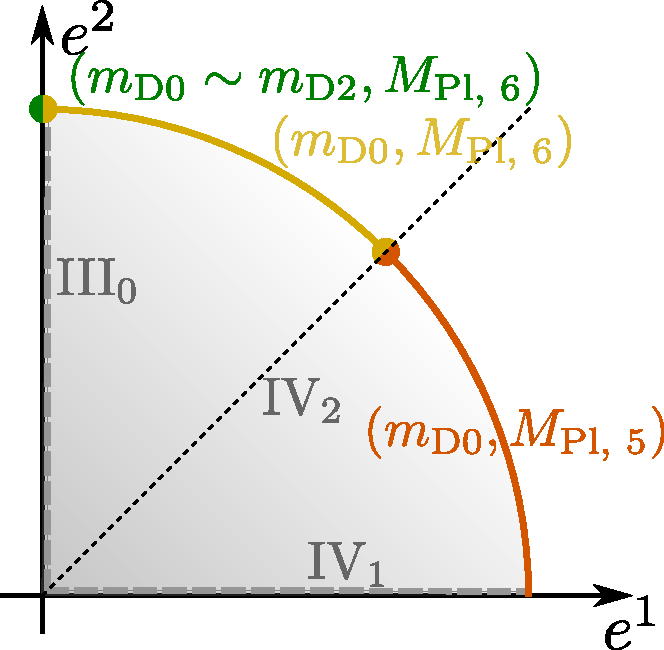
\includegraphics[width=0.4\textwidth]{asympt_lim_IIAN2.pdf}\label{fig:asympt_lim_IIAP11169-lim}
		}
        \quad
	\subfigure[]{
			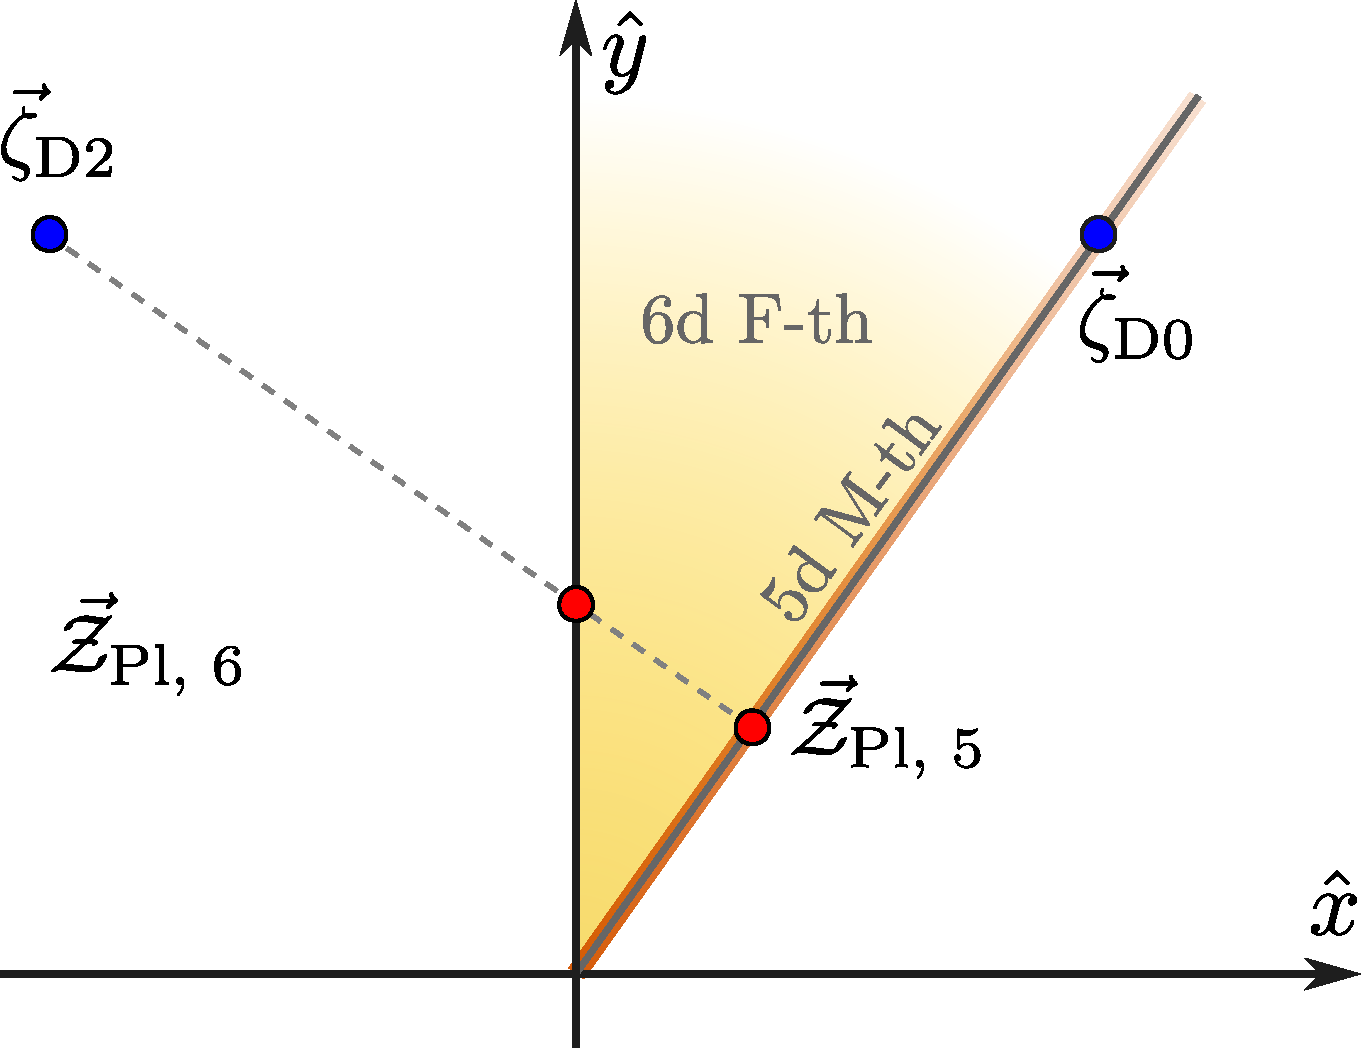
\includegraphics[width=0.5\textwidth]{lim12NEW.pdf}\label{fig:asympt_lim_IIAP11169-vec}
		}
		\caption{\small \textbf{(a)} Classification of infinite distance limits for Type IIA string theory on $\mathbb{P}^{1,1,1,6,9}[18]$ according to their singularity type \cite{Corvilain:2018lgw}, as well as their leading tower and species scales. \textbf{(b)} Relevant scalar charge-to-mass (blue) and species vectors (red) in the flat frame \eqref{eq:flatcoordsP11169}. In particular, one finds $\vec{\zeta}_{\rm D0}=\left(\frac{1}{\sqrt{2}},1\right)$, $\vec{\mathcal{Z}}_{\rm Pl,\; 6}=\left(0, \frac{1}{2}\right)$ and $\vec{\mathcal{Z}}_{\rm Pl,\; 5}=\left(\frac{1}{3\sqrt{2}}, \frac{1}{3}\right)$.}
		\label{fig:asympt lim  IIAP11169}
	\end{center}
\end{figure}	
%%%%%%%%%%%%%%%%
	
	
\subsubsection*{Growth sector $t^1\gg t^2$ with $t^1, t^2 \to \infty$}
	
This includes the particular case of sending $t^1 \to \infty$ with $t^2$ finite (i.e. a type IV$_1$ singularity), since it shares the same leading behaviour of the mass of the towers as well as the species scale. The three-fold volume behaves asymptotically as follows
%
\begin{equation}\label{eq:volP11169n=3}
	\mathcal{V}_{X_3} = \frac{3}{2} (t^1)^3 \left(1 + \mathcal{O}\left(t^2/t^1\right) \right)\, .
\end{equation}
%
%	such that the relevant piece of the moduli space metric behaves as
%
%	\begin{equation}\label{eq:modspacemetricP11169n=3}
	%		G^{-1}\, = \, \left(
	%		\begin{array}{cc}
		%			\frac{(t^1)^3}{t^2} & -3 \frac{(t^1)^3}{t^2}  \\
		%			-3 \frac{(t^1)^3}{t^2} & 9\frac{(t^1)^3}{t^2} \\
		%		\end{array}
		%		\right) \, ,
		%	\end{equation}
%
%	up to quadratic terms on $t^1$. Notice that this metric is ill-defined as stated, since it may be easily checked to have vanishing determinant. This is not an actual problem though, since once we include subleading terms in $1/t^1$ it becomes non-degenerate, and in fact such corrections are indeed essential so as to properly compute the inner products we are interested in here.
Following the discussion of the previous section, this limit corresponds again to decompactifying to 5d M-theory, as expected from being a type IV singularity. %where we may get additional massless states (i.e. vectors and/or hypers) from M2-branes wrapped on the rational curve inside the $\mathbb{P}^2$-base \cite{Gopakumar:1998jq, Witten:1996qb}. %\AC{Sabéis que diferencia en términos microscópicos hay con el large volume point? Si cambias a rescaled coords, el ciclo asociado a $t^2$ se shrinkea en la 5d theory, se trata entonces de un conifold-like point on top of large volume (i.e. hay un e.g. $SU(2)$ enhancement del unique 5d vector multiplet)?},
Thus, it is clear that the pattern will hold along this set of limits due to the general argument given around eq. \eqref{noscale}, but let us show it explicitly here for illustrative purposes. By repeating the same kind of computations as in the previous example we find 
%
\begin{equation}\label{eq:massesD0D2P11169}
	\frac{m_{\text{D0}}}{M_{\text{Pl;}\, 4}} =\sqrt{8\pi } e^{K_{\text{ks}}/2} \sim \frac{1}{(t^1)^{3/2}}\, , \qquad \frac{m_{\text{D2}}}{M_{\text{Pl;}\, 4}} =\sqrt{8\pi } e^{K_{\text{ks}}/2} t^1 \sim \frac{1}{(t^1)^{1/2}}\, ,
\end{equation}
%
for the mass scale of the D0- and D2-particles, respectively. Strictly speaking, there are two possibilities for obtaining four-dimensional BPS states from wrapped D2-branes, since there exist two different non-trivial classes of holomorphic curves within $\mathbb{P}^{1,1,1,6,9}[18]$. The one corresponding to the mass scale computed in \eqref{eq:massesD0D2P11169} is associated to the `horizontal' class, namely the generic fibre of the elliptic fibration. For the other `vertical' class, since the supersymmetric cycle wrapped by the 2-brane is topologically equivalent to a $\mathbb{P}^{1}$-curve that is moreover contractible, there is only a finite number of associated Gopakumar-Vafa (GV) invariants which are non-zero (see e.g., \cite{Candelas:1994hw, Hosono:1993qy}). This means, in turn, that such D2-particles do not give rise to an infinite tower of states becoming massless along the $t^1 \to \infty$ limit, such that we can safely ignore them for our purposes here. 
	
Similarly, as discussed in the previous subsection, the species scale can be computed through D0-brane state counting, arriving at the following result
%
\beq\label{eq:speciesn=3} 
	\frac{\LSP}{M_{\text{Pl;}\, 4}}\, \simeq\, \left( \frac{m_{\text{D0}}}{M_{\text{Pl;}\, 4}} \right)^{1/3} \sim\, \frac{1}{(t^1)^{1/2}}\, ,
\eeq
%
which is nothing but the 5d Planck scale.
	
With this, we now have all the necessary information so as to check whether the condition \eqref{eq:patternP11169} is satisfied or not. Thus, let us first compute the charge-to-mass vectors of the leading tower of states, namely the D0-brane bound states, as well as the species vector obtained from eq. \eqref{eq:speciesn=3} above. The former is given by
%
\beq\label{eq:zetaD0n=3} 
\begin{aligned}
    \vec{\zeta}_{\text{D0}} &= \left( \frac{\left(3t^1+t^2\right)^2}{6 (t^1)^3 + 6 (t^1)^2 t^2 + 2t^1(t^2)^2}\, , \, \frac{3t^1+2t^2}{6 (t^1)^2 + 6 t^1 t^2 + 2(t^2)^2}\right)\\
    &=\left( \frac{3}{2t^1}, \frac{1}{2t^1}\right) + \mathcal{O}\left(t^2/(t^1)^2\right)\, ,
\end{aligned}
\eeq
%
where the notation is $\vec{\zeta}=\left( \zeta_{t^1}, \zeta_{t^2} \right)$. The latter, on the other hand, is simply proportional to the charge-to-mass vector associated to the D0-branes, namely $\vec{\mathcal{Z}}_{\text{sp}}=\frac{1}{3} \vec{\zeta}_{\text{D0}}$. Hence, upon contracting both vectors using the inverse moduli space metric \eqref{eq:fullinversemetric}, one finds that indeed $\vec{\zeta}_{\text{D0}} \cdot \vec{\mathcal{Z}}_{\text{sp}}= \frac{1}{d-2}=\frac{1}{2}$ is verified \emph{exactly}, namely even before performing the expansion in $t^2/t^1$.
	
	
\subsubsection*{Growth sector $t^2\gg t^1$ with $t^1, t^2 \to \infty$}
	
For the other growth sector, the situation turns out to be quite different. First, note that it includes the particular case of sending $t^2 \to \infty$ with $t^1$ finite (i.e. a Type III$_0$ singularity) and, as can be easily checked, the volume \eqref{eq:kahlerpotP11169} is dominated by the last term in the right-hand side
%
\begin{equation}\label{eq:volumen=2limit}
	\mathcal{V}_{X_3} = \frac{1}{2} t^1 (t^2)^2 \left(1 + \mathcal{O}\left(t^1/t^2\right) \right)\, ,
\end{equation}
%
which implies the following asymptotic dependence for the inverse metric components (to leading order in $t^2$)
%
\begin{equation}\label{eq:modspacemetricP11169n=2}
	G^{-1}\, = \, \left(
	\begin{array}{cc}
		2(t^1)^2 & -3 (t^1)^2  \\
		-3 (t^1)^2 & (t^2)^2 \\
	\end{array}
	\right) + \ldots\, .
\end{equation}
%
The QG resolution of the singularity requires from a double decompactification to 6d F-theory on the same elliptic three-fold $X_3$ \cite{Lee:2019wij,Castellano:2022bvr, Marchesano:2022axe}. This may be intuitively understood by looking again at the asymptotic behavior of the mass scales of the infinite towers of light states\footnote{For the D2-branes wrapping the elliptic fibre $k \in \mathbb{Z} \setminus \lbrace 0 \rbrace$ times one obtains \cite{Klemm:2012sx, Klemm:1996hh}
%
\beq \label{eq:GVinvariantsT2limit}
	n_{\textbf{k}} = \chi_E(X_3) = 2 \left ( h^{1,1} (X_3) -  h^{2,1} (X_3) \right)\, ,
\eeq
%
thus behaving like a KK spectrum associated to a circle reduction from 5d to 4d.}
%
\begin{equation}\label{eq:massesD0D2P11169n=2}
	\frac{m_{\text{D0}}}{M_{\text{Pl;}\, 4}}  \sim \frac{1}{\sqrt{t^1} t^2}\, , \qquad \frac{m_{\text{D2}}}{M_{\text{Pl;}\, 4}} \sim \frac{\sqrt{t^1}}{t^2}\, ,
\end{equation}
%
which present both the same dependence, contrary to the previous case (c.f. \eqref{eq:massesD0D2P11169}). Additionally, one can form $\frac{1}{2}$-BPS bound states of D0- and D2-particles upon turning on some (quantized) worldvolume flux $\mathcal{F}$ for the wrapped D2-brane \cite{Polchinski:1998rr}. As a consequence, and following the algorithmic computation of the species scale proposed in Chapter \ref{ch:SpeciesIntro}, one arrives at a cut-off of the form
%
\beq 
	\frac{\LSP}{M_{\text{Pl;}\, 4}} \simeq \left(N_{\text{D0}}\, N_{\text{D2}}\right)^{1/2} \sim \frac{1}{\sqrt{t^2}}\, ,
\eeq
%
where $N_{\text{D2p}}$ counts the number of D$2p$-brane states falling below the species scale. This moduli dependence of the species scale indeed matches with the 6d Planck scale (see discussion around \eqref{eq:6dPlanckscale} below). We can then compute the scalar charge-to-mass vectors for the two towers of states, which to leading order in $1/t^2$, read as
%
\begin{equation}\label{eq:zetavectorsD0D2n=2}
	\vec{\zeta}_{\text{D0}} = \left( \frac{1}{2 t^1}, \frac{1}{t^2} \right) + \mathcal{O}\left(t^1/(t^2)^3\right)\, , \qquad \vec{\zeta}_{\text{D2}} = \left( -\frac{1}{2 t^1}, \frac{1}{t^2} \right) + \mathcal{O}\left(t^1/(t^2)^3\right)\, .
\end{equation}
%
Analogously, one finds for the species vector
%
\begin{equation}\label{eq:speciesvectorIIA}
	\vec{\mathcal{Z}}_{\text{sp}} = \left( \frac{3}{4 t^2}, \frac{1}{2t^2} \right) + \mathcal{O}\left(t^1/(t^2)^3\right)\, ,
\end{equation}
%
such that upon taking the product with respect to the inverse metric \eqref{eq:modspacemetricP11169n=2}, the pattern \eqref{eq:pattern} still holds for \emph{both} towers. In this case, however, it turns out being crucial to take into account that $t^1/t^2 \to 0$ asymptotically along the limit of interest. 
	
	
\subsubsection{General story}
\label{sss:IIA/Fthy}
	
The previous example contained two types of limits, one belonging to the category of Section \ref{ss:typeIVlimits} and a new one: A partial decompactification to 6d F-theory. Let us elaborate a bit more on this second case, which corresponds to the regime where $t^2$ grows faster than $t^1$. From \eqref{eq:modspacemetricP11169n=2}, one can check that the length of relevant vectors associated to the tower of bound states behave as follows
%
\begin{equation}
	|\vec{\zeta}_{\text{eff}}|= \left|\frac{1}{2} (\vec{\zeta}_{\text{D0}} + \vec{\zeta}_{\text{D2}}) \right|= 1 + \mathcal{O}\left( \left(t^1/t^2\right)^2\right)\, , \qquad
	|\vec{\mathcal{Z}}_{\text{sp}}| = \frac{1}{2} + \mathcal{O}\left( \left(t^1/t^2\right)^2\right)\, ,
\end{equation}
%
which indeed coincide with the typical values for Kaluza-Klein vectors associated to a two-dimensional compact manifold, matching with the microscopic interpretation of the singularity as a decompactification from 4d to 6d. Our aim here will be to show that this is generically the case whenever we explore a type $\mathbf{T}^2$ limit in the language of \cite{Lee:2019wij} (or a Type III singularity in the language of \cite{Grimm:2018ohb}). Subsequently, this will allow us to argue that the pattern $\eqref{eq:pattern}$ holds in general for such kind degenerations. 
	
Let us consider an infinite distance limit in which the curve associated to the fastest growing modulus has the intersection numbers of a Type III singularity (see second row in Tables \ref{tab:intersN=2} and \ref{tab:limitsN=2}). Geometrically, this corresponds to a limit in which the Calabi--Yau three-fold exhibits an elliptic fibration  over a K\"ahler surface $B_2$
%
\begin{equation}\label{eq:ellfibration}
			\begin{aligned}
				\pi: \qquad \mathbf{T}^2 \hookrightarrow &\;X_{3} \\
				&\;\; \downarrow \qquad , \\ &\ \ B_{2}
			\end{aligned}
\end{equation}
%
where the volume of the latter grows faster than the fiber (i.e.  belongs to the type $\mathbf{T}^2$ class).
After resolving any Kodaira-Néron type of singularity that may be present \cite{Weigand:2018rez}, we can then divide the K\"ahler moduli into two sets: those parametrizing fibral curves, $\lbrace t^a_f \rbrace$, and the ones inherited from the base, $\lbrace t^{\alpha}_b \rbrace$. These fields arise as the expansion coefficients of the K\"ahler 2-form $J$ over a basis $\lbrace \omega_A \rbrace = \lbrace \omega_a, \omega_{\alpha} \rbrace$ of $H^{1,1}(X_3, \mathbb{Z})$, as follows
%
\begin{equation}
		J= t^A \omega_A = t^a_f \omega_a + t^{\alpha}_b \omega_{\alpha} \, , 
\end{equation}
%
with $\alpha=1,\ldots, h^{1,1}(B_2)$, whilst the index $a$ runs from 1 to $n$, with $n-1$ being the sum of the ranks of the Mordell-Weil group and the non-Abelian gauge algebras realized at co-dimension one degenerations $\Delta \subset B_2$ \cite{wazir_2004}.
Therefore, the limit we want to study corresponds to
%
\begin{equation}\label{eq:n=2limit}
	t^a_f = \text{const.}\, , \qquad t^{\alpha}_b = \xi^{\alpha} \sigma\, , \qquad \text{with}\, \, \sigma\to \infty\, , 
\end{equation}
%
accompanied by a suitable co-scaling of the 10d dilaton --- so as to keep fixed all moduli in the hypermultiplet sector. Microscopically, the quantum gravity resolution of the singularity requires from a double decompactification to F-theory on the same elliptic three-fold $X_3$, as we review in the following.
	
On the one hand, at the level of the spectrum, one finds --- at least in the simplest instances --- only two infinite sets of asymptotically light states: those comprised by D0-branes and D2-branes wrapping the elliptic fibre class. Notice that, since the volume of the latter 2-cycle, which we denote by $\mathcal{V}_{\mathbf{T}^2}$, does not diverge in the limit \eqref{eq:n=2limit}, the central charges associated to both towers of states are controlled by the same quantity, namely the (square root of the) overall three-fold volume:
%
\begin{equation}\label{eq:massesD0D2Fthylimit}
	\frac{m_{\text{D0}}}{M_{\text{Pl;}\, 4}}  = \sqrt{\frac{\pi}{\mathcal{V}_{X_3}}}\, , \qquad \frac{m_{\text{D2}}}{M_{\text{Pl;}\, 4}} = \sqrt{\frac{\pi}{\mathcal{V}_{X_3}}}\, \mathcal{V}_{\mathbf{T}^2}\, .
\end{equation}
%
and indeed they furnish the Kaluza-Klein replica along the torus of the 6d F-theory massless fields. 
	
From this set of asymptotically light towers, one can easily compute the species scale dominating the infinite distance limit. In fact, upon using Type IIA/F-theory duality \cite{Lee:2019wij}, we conclude that the species scale should be controlled parametrically by the six-dimensional Planck mass, namely\footnote{The second equality in \eqref{eq:6dPlanckmass} follows from the moduli identifications $R_5 = \mathcal{V}_{X_3}^{1/3}$ (c.f. \eqref{eq:modulimatching}) as well as $R_6^{-4/3}=\frac{\mathcal{V}_{\mathbf{T}^2}}{\mathcal{V}_{X_3}^{1/3}}$ \cite{Corvilain:2018lgw}.}
%
\beq \label{eq:6dPlanckmass}
	M_{\text{Pl; 6}}^2 \simeq\frac{M_{\text{Pl;}\, 4}^2}{R_6^{2/3}R_5} = \frac{M_{\text{Pl;}\, 4}^2 \mathcal{V}_{\mathbf{T}^2}^{1/2}}{\mathcal{V}_{X_3}^{1/2}} \sim \frac{1}{\sigma^{1/2}}\, ,
\eeq
%
with $R_6$ and $R_5$ being the corresponding radii of the 6d-to-5d and 5d-to-4d circle compactifications (measured in the 6d and 5d Planck units respectively). Indeed, one can check that
%
\beq\label{eq:6dPlanckscale}
	\left(\frac{M_{\text{Pl; 6}}}{M_{\text{Pl;}\, 4}}\right)^2 \simeq \left( \frac{m_{\text{D0}}\, m_{\text{D2}}}{M_{\text{Pl;}\, 4}^2}\right)^{\frac{1}{2}} \sim \left(\frac{\LSP}{M_{\text{Pl;}\, 4}}\right)^2\, ,
\eeq
%
in agreement with the usual species counting computation. 
	
On the other hand, for the K\"ahler potential one finds the following leading asymptotic behavior \cite{Lee:2019wij,Cota:2022maf}
%
\begin{equation}\label{eq:kahlerpotn=2}
	K_{\text{ks}}= - \log \left(\frac{1}{2} \left( c_a t^a_f\right)\eta_{\alpha \beta} t_b^{\alpha} t_b^{\beta} + \mathcal{O} (\sigma)\right)\, ,
\end{equation}
%
where $c_a$ are some positive coefficients\footnote{\label{fnote:ellipticclass}The coefficients $c_a$ in eq. \eqref{eq:kahlerpotn=2} determine the generic elliptic fibre class $[\mathcal{C}_{\mathbf{T}^2}]$. Hence, in terms of a basis $\lbrace \mathcal{C}_f^a \rbrace$ of generators of the relative Mori cone $\mathsf{Mori}(X_3/B_2)$, the former becomes $\mathcal{C}_{\mathbf{T}^2}= \sum_a c_a \mathcal{C}_f^a$, where the notation follows that of \cite{Cota:2022maf}.} determined by the particular fibration structure of the three-fold and $\eta_{\alpha \beta}$ denote the intersection numbers of the two-fold base \cite{Corvilain:2018lgw}. Notice, in particular, that the basis $\lbrace \omega_A\rbrace = \lbrace \omega_a, \omega_{\alpha} \rbrace$ verifies that $\omega_a \wedge \omega_b \wedge \omega_c = \mathcal{K}_{a b c}=0$. Therefore, upon inserting the leading order expansion \eqref{eq:kahlerpotn=2} into the definition of the vector multiplet metric $G_{A B}$, one finds
%
%\begin{equation}\label{eq:metricn=2}
\begin{align}\label{eq:metricn=2}
	G_{\alpha \beta} &= \frac{1}{2} \frac{\partial^2 K_{\text{ks}}}{\partial t^{\alpha}_b \partial t^{\beta}_b} = G^{(\rm lead.)}_{\alpha \beta} + \mathcal{O}\left(1/\sigma^3 \right)\, , \quad G_{\alpha b} = \frac{1}{2} \frac{\partial^2 K_{\text{ks}}}{\partial t^{\alpha}_b \partial t^{b}_f} = G^{(\rm lead.)}_{\alpha b} + \mathcal{O}\left(1/\sigma^2 \right)\, ,\notag\\
	G_{a b} &= \frac{1}{2} \frac{\partial^2 K_{\text{ks}}}{\partial t^a_f \partial t^b_f} = G^{(\rm lead.)}_{a b} + \mathcal{O}\left(1/\sigma \right)\, ,
\end{align}
%\end{equation}
%
with the following explicit expression for the leading-order matrices in eq. \eqref{eq:metricn=2} above
%
\begin{align}\label{eq:constmatricesn=2lim}
	\notag G^{(\text{lead.})}_{\alpha \beta} &=\frac{2 \left(\mathcal{K}_{\alpha \gamma a} t_b^{\gamma} t^a_f\right) \left( \mathcal{K}_{\beta \delta b} t_b^{\delta} t^b_f\right)}{\left( \mathcal{K}_{a \gamma \delta} t^a_f t_b^{\gamma} t_b^{\delta} \right)^2} - \frac{\mathcal{K}_{\alpha \beta a} t^a_f}{\mathcal{K}_{a \gamma \delta} t^a_f t_b^{\gamma} t_b^{\delta}}\, , \quad G^{(\text{lead.})}_{a b} =\frac{\left(\mathcal{K}_{a \alpha \beta} t_b^{\alpha} t_b^{\beta}\right) \left( \mathcal{K}_{b \gamma \delta} t_b^{\gamma} t_b^{\delta}\right)}{2\left( \mathcal{K}_{a \gamma \delta} t^a_f t_b^{\gamma} t_b^{\delta} \right)^2}\, ,\\
    G^{(\text{lead.})}_{\alpha b} &=\frac{\left(\mathcal{K}_{\alpha \beta a} t_b^{\beta} t^a_f\right) \left( \mathcal{K}_{b \gamma \delta} t_b^{\gamma} t_b^{\delta}\right)}{\left( \mathcal{K}_{a \gamma \delta} t^a_f t_b^{\gamma} t_b^{\delta} \right)^2} - \frac{\mathcal{K}_{\alpha b \gamma} t_b^{\gamma}}{\mathcal{K}_{a \gamma \delta} t^a_f t_b^{\gamma} t_b^{\delta}}\, ,
\end{align}
%
where $\mathcal{K}_{a \alpha \beta} = c_a \eta_{\alpha \beta}$. It is easy to see that these matrices have full rank except for $G^{(\rm lead.)}_{a b}$, which has rank one.\footnote{Actually, the (sub-)matrix $G^{(\text{lead.})}_{\alpha b}$, despite having full rank in general, can be identically zero in special circumstances, given that there are two terms with opposite sign in eq. \eqref{eq:constmatricesn=2lim}. This is the case when e.g., the fibration is non-degenerate, as happens in the two-moduli example discussed in Section \ref{sss:ExampleII}.}
	
Armed with all this, one can readily check upon using the no-scale property of the metric $G^{(\text{lead.})}_{\alpha \beta}$, namely the identity%\footnote{The identity \eqref{eq:noscale} follows from the more familiar no-scale condition for a two-fold, namely $K_{\alpha} K^{\alpha \bar \beta} K_{\bar \beta}=2$, upon taking into account that $G_{\alpha \beta} = 2 K_{\alpha \bar \beta}$.}
%
\begin{equation}\label{eq:noscale}
	\frac{\partial K_{\text{ks}}}{\partial t^{\alpha}_b} G_{(\text{lead.})}^{\alpha \beta} \frac{\partial K_{\text{ks}}}{\partial t^{\beta}_b} = 4\, ,
\end{equation}
%
that the product
%
\begin{equation}
	\vec{\zeta}_{\text{D0, D2}}\cdot\vec{\mathcal{Z}}_{\rm sp}=\left(G^{A B}\partial_{A}\log m_{\text{tower}}\,\partial_{B}\log \Lambda_{\rm sp}\right) \stackrel{~\eqref{eq:n=2limit}~}{=} \frac{1}{2}\, , \qquad A, B= \lbrace a, \beta \rbrace\, ,
\end{equation}
%
is indeed satisfied for any trajectory of the form specified in \eqref{eq:n=2limit} above. To see this, it is important to realize that any term involving derivatives with respect to the fibral moduli, $\{t^a_f\}$, provides ultimately a contribution to the scalar product $\vec{\zeta}_{\text{t}}\cdot\vec{\mathcal{Z}}_{\rm sp}$ which is of $\mathcal{O}\left(1/\sigma\right)$ or higher, such that it goes away upon taking the infinite distance limit. For this same reason, the result also applies to more general cases in which the fiber volume is also sent to infinity, but at a slower rate than that of the base.
	
\subsection{Type II limits: Emergent string limits}
\label{ss:typeIIlimits}
	
\subsubsection{Example 3: Type IIA on $\mathbb{P}^{1,1,2,2,6} [12]$}
\label{sss:ExampleIII}
	
As our final example, we consider Type IIA string theory compactified on the three-fold $X_3=\mathbb{P}^{1,1,2,2,6}$ [12]. Topologically, such two-parameter CY$_3$ can be seen as a $K3$ fibration over a $\mathbb{P}^1$-base, whose K\"ahler moduli $\lbrace t^1, t^2 \rbrace$ appear in the K\"ahler potential as follows\footnote{Here $t^2$ measures the classical volume of the $\mathbb{P}^1$-base, whilst $t^1$ parameterizes the volume of a second $\mathbb{P}^1$ corresponding to a rational curve (of non-negative self-intersection) inside the $K3$-fibre \cite{Candelas:1993dm}.}
%
\begin{equation}\label{eq:kahlerpotP11226}
	e^{-K_{\text{ks}}} = \frac{16}{3}(t^1)^3 + 8(t^1)^2 t^2 + \ldots\, ,
\end{equation}
%
where the ellipsis denotes further $\alpha'$ as well as worldsheet instanton corrections, which are both suppressed in the large volume patch. The explicit (inverse) moduli space metric that derives from the K\"ahler potential above is given by 
%
\begin{equation}\label{eq:fullinversemetricP11226}
	G^{-1}\, = \, \left(
	\begin{array}{cc}
		(t^1)^2 & - \frac{2}{3} (t^1)^2  \\
		- \frac{2}{3} (t^1)^2 & \frac{4}{3}(t^1)^2+\frac{8}{3} t^1 t^2 +2 (t^2)^2 \\
	\end{array}
	\right) \, .
\end{equation}
% 
Using the nomenclature of MHS, we have the following infinite distance limits (see e.g., \cite{kerr2019polarized, Bastian:2021eom}): \emph{(i)} $t^1 \to \infty$ with $t^2$ finite (a Type IV$_2$ singularity), \emph{(ii)} $t^2 \to \infty$ with $t^1$ finite (a Type II$_1$ singularity), and \emph{(iii)} $t^1,t^2 \to \infty$ (a Type IV$_2$ singularity). The type IV singularities will again correspond to M-theory circle decompactifications, so the analysis of Section \ref{sss:IIA/Mthy} carries over. In fact, as it was the case in the example from Section \ref{sss:ExampleII}, all $t^2$--\,dependence disappears when taking the limit $t^1\gg t^2 \gg 1$, such that the moduli space becomes effectively one-dimensional. In addition, one may define global flat coordinates for the slice parametrized by $\lbrace t^1, t^2\rbrace$, which read
%
\begin{equation}\label{e:mod 11226}
 \begin{aligned}
     \hat{x} &= \frac{1}{3}\log \left(2 (t^1)^3\right)\, , \qquad \hat{y} =\frac{1}{\sqrt{2}}\log \left( \frac{2t^1+3t^2}{2^{2/3}}\right)\, ,
 \end{aligned}
\end{equation}
%
with the restriction that $\hat{y} \geq \frac{1}{\sqrt{2}}\hat{x}\geq 0$. These can then be used to depict the different relevant $\zeta$- and $\mathcal{Z}$-vectors in the present set-up, as shown in Figure \ref{fig:asympt lim  IIAP1126}. Let us stress that the regime $t^1\gtrsim t^2 \gg 1$ is mapped again to the boundary $\{\hat{y}=\frac{1}{\sqrt{2}}\hat{x}\}$, ensuring that the bound \eqref{eq:SSDC4d} is non-trivially satisfied. %For clarity reasons, however, we will use the $\{t^1, t^2\}$ coordinates in our subsequent analysis.
	
On the other hand, things get more interesting upon probing the limit $t^2 \to \infty$ (either with $t^1$ fixed or growing at a smaller rate), since the QG resolution of the corresponding Type II singularity is of a different kind than the ones discussed so far. The purely geometric analysis of \cite{Lee:2019wij} shows that it  corresponds to an emergent string limit, in which a critical Heterotic string arising from a NS5-brane wrapping the $K3$-fibre \cite{Harvey:1995rn} becomes asymptotically tensionless at the infinite distance boundary. It is thus clear that the pattern \eqref{eq:pattern} is also satisfied in this case, since the species scale is set by the string scale, whose exponential rate must be given by $\frac{1}{\sqrt{d-2}}$ --- if corresponding to a fundamental string propagating in $d$ dimensions. Nevertheless, let us check this explicitly by computing the relevant vectors within this regime. We first calculate the leading contribution to the three-fold volume in \eqref{eq:kahlerpotP11226}, which asymptotically scales as follows 
%
\begin{equation}\label{eq:volTypeIIlimit}
	\mathcal{V}_{X_3} = 2 (t^1)^2\, t^2 \left(1 + \mathcal{O}\left(t^1/t^2\right) \right)\, .
\end{equation}
%
Next we need to determine both the charge-to-mass vectors associated to the leading tower of states and the appropriate species scale. There is indeed a plethora of potentially light towers, both of perturbative and non-perturbative nature. First of all, one finds a critical string arising from a NS5-brane wrapped on the $K3$ surface, whose tension behaves as
%
\begin{equation}
	T_{\text{NS5}} = \frac{2\pi}{ \ell_s^2 g_s^2} \mathcal{V}_{K3}\, ,
\end{equation}
%
with $\ell_s = 2\pi \sqrt{\alpha'}$ being the fundamental string length and $\mathcal{V}_{K3}= (t^1)^2$ denotes the volume of the $K3$-fibre. Notice that along the $t^2$--\,limit that we consider here, the volume of the fibre either remains constant or grows at a smaller rate. %\footnote{Interestingly, as explained in \cite{Lee:2019wij}, upon looking at the analytic continuation of the period vectors from the Large Volume Point to the vicinity of the Type II$_1$ singularity, one finds that there is an obstruction to taking the vanishing fibre limit, whose volume remains constant (or grows at a parametrically slower rate) and of $\mathcal{O}(1)$ in string units \cite{Lerche:1997,Curio:2000sc}.} 
Hence, upon properly co-scaling the 10d dilaton so as to keep its 4d counterpart fixed and finite (see discussion at the end of Section \ref{ss:preliminary}) one arrives at %the following asymptotic behavior
%
\begin{equation}\label{eq:NS5vector}
	\frac{T_{\text{NS5}}}{M_{\text{Pl;}\, 4}^2} = \frac{\mathcal{V}_{K3}}{ 2 \mathcal{V}_{X_3}} \sim \frac{1}{t^2} \quad \Longrightarrow \quad \vec{\zeta}_{\text{osc, NS5}} = \vec{\mathcal{Z}}_{\text{osc, NS5}} = \left( \frac{1}{3t^2}, \frac{1}{2 t^2} \right) + \mathcal{O}\left( t^1/(t^2)^2\right)\, .
\end{equation}
%
%thus leading to a charge-to-mass vector which at leading order reads
%
%\begin{equation}
%	\vec{\zeta}_{\text{NS5}} = \vec{\mathcal{Z}}_{\text{NS5}} = \left( \frac{1}{3t^2}, \frac{1}{2 t^2} \right)\, .
%\end{equation}
%
%which holds at leading order in $t^1/t^2$. 
Apart from these, there are also additional infinite towers of states which become asymptotically massless in the limit of interest. These can be seen to correspond to Kaluza-Klein modes associated to the diverging $\mathbb{P}^1$-base, with characteristic mass
%
\begin{equation}\label{eq:KKP1scale}
	\frac{m^2_{\text{KK}, \, \mathbb{P}^1}}{M_{\text{Pl;}\, 4}^2} = \frac{e^{2\varphi_4}}{4 \pi \mathcal{V}_{\mathbb{P}^1}} \sim \frac{1}{t^2}\, ,
\end{equation}
%
as well as non-perturbative states arising from D0- and D2-branes wrapping the rational curve within the $K3$-fibre, %\footnote{The tower of D2-branes wrapping $n \in \mathbb{Z} \setminus \lbrace 0 \rbrace$ times the $\mathbb{P}^1$-curve inside $K3$ are mapped through M-theory/Heterotic duality \cite{Kachru:1995wm} to winding and KK modes of the dual heterotic string on $\widehat{K3} \times \mathbf{T}^2$ along the circle \cite{Harvey:1995fq, Kawai:1996te}.} 
whose masses scale as follows
%
\begin{equation}\label{eq:D0D2emergenthet}
	\frac{m_{\text{D0}}}{M_{\text{Pl;}\, 4}} = \frac{\sqrt{\pi}}{\mathcal{V}_{X_3}^{1/2}}\sim \frac{1}{t^1 (t^2)^{1/2}}\, , \qquad \frac{m_{\text{D2}}}{M_{\text{Pl;}\, 4}} = \frac{\sqrt{\pi} t^1}{\mathcal{V}_{X_3}^{1/2}}\sim \frac{1}{(t^2)^{1/2}}\, .
\end{equation}
%
%In terms of scalar charge-to-mass vectors, one would then write
%
%\begin{align}
%	\vec{\zeta}_{\text{KK}, \, \mathbb{P}^1} &= \left( 0, \frac{1}{2 t^2} \right)\, , \qquad 
%  \vec{\zeta}_{\text{D0}} = \left( \frac{1}{t^1}, \frac{1}{2 t^2} \right)\, ,\notag\\
%    \vec{\zeta}_{\text{D2}} &= \left( 0, \frac{1}{2 t^2} \right)\, .
%\end{align}
%
The latter infinite set of D2-branes are mapped through Type IIA/Heterotic duality (c.f. Section \ref{ss:dualitieswithlowersusy}) to winding modes of the dual Heterotic string on $\widehat{K3} \times \mathbf{T}^2$ \cite{Harvey:1995fq, Kawai:1996te}. Note that all these towers decay at the same rate than the emergent string along the limit $t^2\to \infty$ with $t^1$ fixed.
	
From the above mass formulae one may readily compute the associated charge-to-mass vectors upon taking derivatives with respect to the non-compact K\"ahler fields,\footnote{Strictly speaking, the vector $\vec{\zeta}_{\text{KK},\, \mathbb{P}^1}$ presents an additional non-trivial component due to the dependence of the KK scale on the 4d dilaton in \eqref{eq:KKP1scale}. Such component, despite not contributing to the inner product \eqref{eq:patternemergentheterotic} below, must be taken into account when computing the length of the charge-to-mass vector, which then matches eq. \eqref{eq:zeta&speciesveconemodulus} for $d=4$ and $n=2$.} yielding
%
\begin{equation}\label{eq:zetavectorsn=1}
\begin{aligned}
	\vec{\zeta}_{\text{KK},\, \mathbb{P}^1} &= \left( 0, \frac{1}{2 t^2} \right)\, , \qquad \vec{\zeta}_{\text{D0}} = \left( \frac{1}{t^1}, \frac{1}{2 t^2} \right) + \mathcal{O}\left( t^1/(t^2)^2\right)\, ,\\
    \vec{\zeta}_{\text{D2}} &= \left( \frac{1}{3t^2}, \frac{1}{2 t^2} \right) + \mathcal{O}\left( t^1/(t^2)^2\right)\, .
\end{aligned}
\end{equation}
%
Therefore, taking into account that the species counting is dominated by the excitation modes of the dual Heterotic string, such that $\vec{\mathcal{Z}}_{\text{sp}}=\vec{\mathcal{Z}}_{\text{osc, NS5}}$, one can explicitly check that
%
\begin{equation}\label{eq:patternemergentheterotic}
	\vec{\zeta}_{\text{t}} \cdot \vec{\mathcal{Z}}_{\text{osc, NS5}} = \frac{1}{2}\, ,
\end{equation}
%
where $\text{t}\in \lbrace \text{KK, D0, D2, NS5} \rbrace $ includes all the light leading towers, and we have made use of the inverse metric shown in eq. \eqref{eq:fullinversemetricP11226}. In fact, the above inner product holds exactly (i.e. even before taking the infinite distance limit) for all charge-to-mass vectors except for $\vec{\zeta}_{\text{KK},\, \mathbb{P}^1}$, in which case \eqref{eq:pattern} is satisfied at leading order in $t^1/t^2$.
	
%%%%%%%%%%%%%%%%
\begin{figure}[htb]
	\begin{center}
	\subfigure[]{
			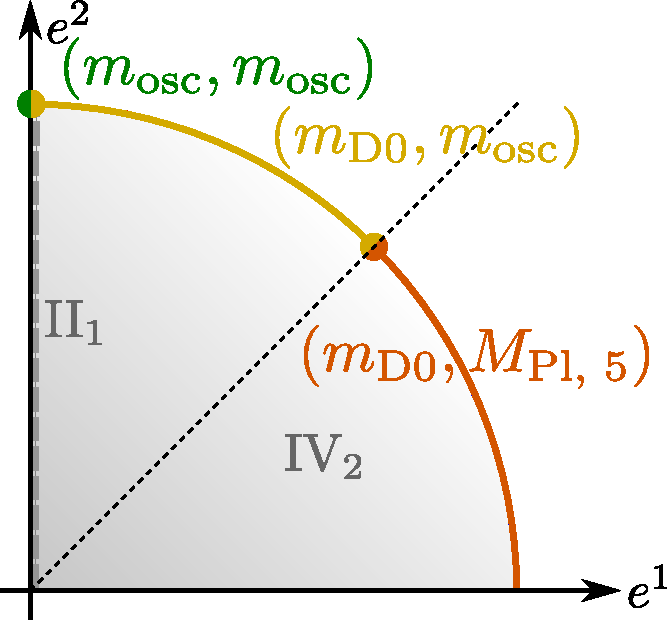
\includegraphics[width=0.4\textwidth]{asympt_lim_IIAP1126.pdf}\label{fig:asympt_lim_IIAP1126-lim}
		}
        \quad
	\subfigure[]{
			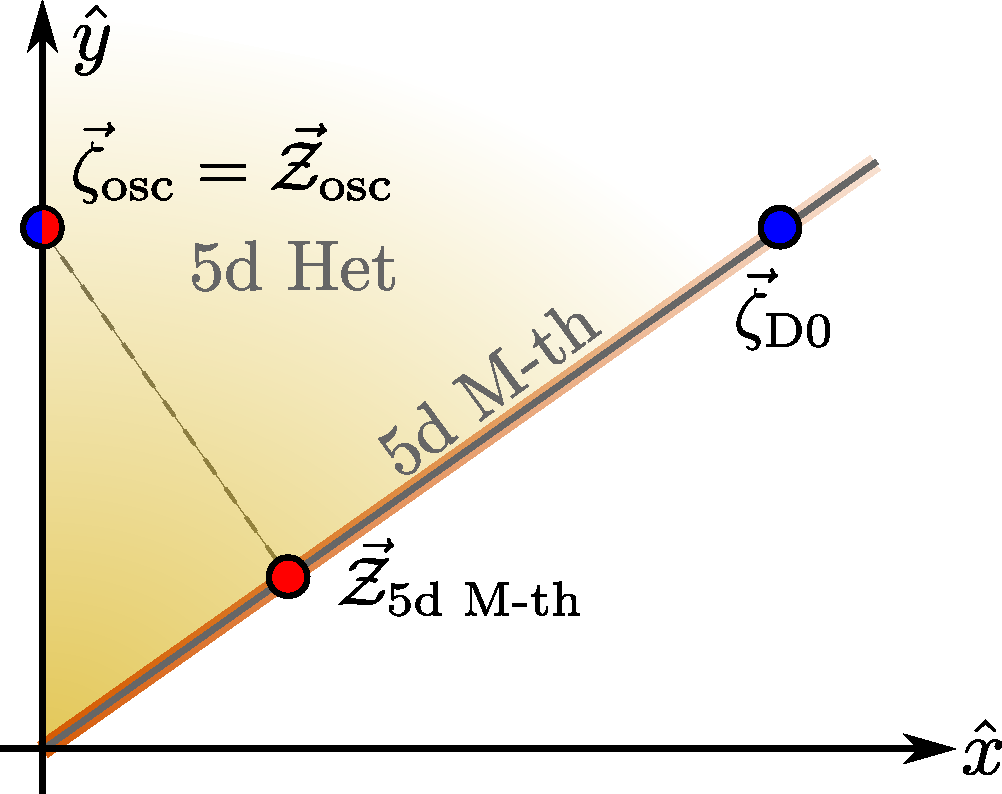
\includegraphics[width=0.45\textwidth]{lim2.pdf}\label{fig:asympt_lim_IIAP1126-vec}
		}
		\caption{\small \textbf{(a)} Classification of infinite distance limits for Type IIA string theory on $\mathbb{P}^{1,1,2,2,6}[12]$ according to their singularity type \cite{Corvilain:2018lgw}, as well as their leading tower and species scales. \textbf{(b)} Relevant scalar charge-to-mass (blue) and species vectors (red) in the flat frame \eqref{e:mod 11226}. In particular, one finds $\vec{\zeta}_{\rm osc}=\vec{\mathcal{Z}}_{\rm osc}=\left(0,\frac{1}{\sqrt{2}}\right)$, $\vec{\zeta}_{\rm D0}=\left(1,\frac{1}{\sqrt{2}}\right)$ and $\vec{\mathcal{Z}}_{\rm Pl,\; 5}=\left(\frac{1}{3}, \frac{1}{3\sqrt{2}}\right)$.}
		\label{fig:asympt lim  IIAP1126}
	\end{center}
\end{figure}	
%%%%%%%%%%%%%%%%%%%	

To summarize, consider some limit of the form $\mathbf{t}(\sigma) = \left( t^1, t^2 \right) = \left(\sigma^{e^1}, \sigma^{e^2}\right)$, with the vector $\mathbf{e}$ belonging to the first quadrant of $\mathbf{S}^1$. If  $e^2 > e^1$, we get an emergent string limit and the analysis presented above readily applies. If $e^1 \geq e^2$, we rather decompactify to 5d M-theory and the general argument of Section \ref{sss:ExampleI} carries over so that the pattern equally holds. In Figure \ref{fig:asympt_lim_IIAP1126-lim} these limits, as well as the leading towers and species, are depicted, while in \ref{fig:asympt_lim_IIAP1126-vec} the associated scalar charge-to-mass vectors (which are constant in flat coordinates) are represented. Hence, the pattern
%
\begin{equation}\label{eq:patternP11226}
	\left.\vec{\zeta}_{\text{t}}\cdot\vec{\mathcal{Z}}_{\rm sp}\right|_{\mathbf{t}(\sigma)}=\left.\left(G^{a b}\partial_{a}\log m_{\text{tower}}\,\partial_{b}\log \Lambda_{\rm sp}\right)\right|_{\mathbf{t}(\sigma)} = \frac{1}{2}\, ,
\end{equation}
%
is verified for any such asymptotic trajectory $\mathbf{t}(\sigma)$. 
	
Finally, let us remark here that some of the towers of particles arising in the present set-up, such as the one associated to $m_{\text{KK}, \, \mathbb{P}^1}$, suffer from the \emph{sliding} phenomenon first described within the Heterotic string theory context in ref. \cite{Etheredge:2023odp} (c.f. Section \ref{ss:het s1}). Moreover, note that the charge-to-mass and species vectors arrangement in Figure \ref{fig:asympt_lim_IIAP1126-vec} corresponds to a rotated version of that shown in Figure \ref{sfig:KKstring}, thus making manifest that they both share the same physical origin.

\subsubsection*{The Seiberg-Witten point and worldsheet instantons}

It is interesting at this point to extend the previous large volume analysis to other infinite distance degenerations which crucially require from both perturbative and non-perturbative $\alpha'$-corrections so as to be properly defined. The simplest such instance happens actually in the present $\mathbb{P}^{1,1,2,2,6} [12]$ example, when sitting close to the Seiberg-Witten singularity \cite{Seiberg:1994rs}. This can be reached upon considering the intersection locus between the conifold discriminant and the $t^2 \to \infty$ divisor, see e.g., \cite{Kachru:1995fv, Curio:2000sc} for details. In what follows, it will be convenient to introduce some local patch which vanish by construction at Seiberg-Witten point, as follows
%
\beq \label{eq:normalcoords}
	z^1=1-1728\, e^{b^1+\i t^1}\, , \qquad z^2= \frac{4\, e^{b^2+\i t^2}\, 1728^2 \left(e^{b^1+\i t^1} \right)^2}{\left( 1-1728\, e^{b^1+\i t^1}\right)^2}\, .
\eeq
%
Indeed, the singularity located at $z^1=z^2=0$ lies at infinite distance in the full K\"ahler metric (i.e. taking into account worldsheet instantons), and therefore the relation \eqref{eq:pattern} should hold as well. This limit is moreover closely related to the one previously discussed, with the crucial difference that now the fibre volume reaches its minimum possible value --- which is of stringy size \cite{Aspinwall:1993xz, Greene:1996tx,Greene:2000ci}, whilst that of the $\mathbb{P}^1$-base remains divergent. Hence, in order to check the pattern we need to know both the asymptotic form of the moduli space metric as well as the period vector close to the Seiberg-Witten point. These had been already computed and thoroughly studied in the literature, so we will only need to adapt the relevant results for our purposes here. %We choose to follow the notation and conventions introduced in \cite{Bastian:2021eom}, but we will also need to compare at several instances with the quantities computed in \cite{Lee:2019wij}.

Let us consider first the periods expanded around the point of interest. After solving the Picard-Fuchs system of differential equations \cite{Cox:2000vi,Hori:2003ic}, one finds the following convenient basis of solutions (in the coordinate frame \eqref{eq:normalcoords})
%
\begin{equation} \label{eq:periodvectorPicardFuchs}
    \varpi_{\rm sw} = \frac{1}{\pi} \begin{pmatrix}
    1 + \frac{5}{36} z^1 \\
    z^1 \\
    -\sqrt{z^1} \\
   \frac{\i}{\pi} \left(\log(z^2) - 6 \log2 + 7\right) \sqrt{z^1}\\
   \frac{\i}{2\pi} \left(5+\log \left(z^2 (z^1)^2 \right)\right) \left( 1 + \frac{5}{36} z^1\right)\\
   \frac{\i}{2\pi} \left(1 + \log \left(z^2 (z^1)^2 \right)\right) z^1
\end{pmatrix}\, ,
\end{equation}
%
where we only display the leading order terms in an expansion around $z^1=z^2=0$. Next, one needs to perform some analytic continuation translating the basis of integral periods around the large volume point to the Seiberg-Witten locus. This can be done upon multiplying \eqref{eq:periodvectorPicardFuchs} by the matrix \cite{Lee:2019wij}
%
\begin{equation} \label{eq:analyticContmatrix}
    \mathsf{M} = \begin{pmatrix}
       \frac{1}{2\mathcal{X}} & \frac{\mathcal{X}}{2} & \frac12 & 0 & 0 & 0 \\
    \frac{\i}{2\mathcal{X}} & -\frac{\i \mathcal{X}}{2} & 0 & 0 & 0 & 0 \\
    \i \left( \xi_1 + \frac{\xi_2}{\mathcal{X}^2}\right) & \i \left( \xi_3 + \xi_4 \mathcal{X}^2\right) & 0 & 1 & -\frac{1}{2\mathcal{X}} & -\frac{\mathcal{X}}{2} \\
    \frac{1}{\mathcal{X}} & \mathcal{X} & 0 & 0 & 0 & 0 \\
    -2\xi_1 + \frac{2\xi_2} {\mathcal{X}^2} & 2 \xi_3-2\xi_4 \mathcal{X}^2 & 0 & 0 & \frac{\i}{\mathcal{X}} & -\i \mathcal{X} \\
    0 & 0 & 0 & 2 & 0 & 0
\end{pmatrix}\, ,
\end{equation}
%
where $\mathcal{X}=\frac{\Gamma \left( \frac34 \right)^4}{\sqrt{3} \pi^2}$ and $\{\xi_i \}$ are numerical constants given by
%
\beq
	\xi_1 = -4.16688\, , \quad \xi_2 =0.130737\, , \quad \xi_3 = -0.99488\, , \quad \xi_4 = 7.51362\, ,
\eeq
%
which yields the following (leading-order) period vector 
%
\begin{equation} \label{eq:periodvectorSW}
    \Pi_{\rm sw} = \begin{pmatrix}
    X^0 \\
           X^1 \\
           X^2\\
           \mathcal{F}_1 \\
           \mathcal{F}_2\\
           \mathcal{F}_0
\end{pmatrix} := \frac{1}{\pi} \begin{pmatrix}
    \frac{1}{2\mathcal{X}}\\
    \frac{\i}{2\mathcal{X}} \\
    -\frac{\i}{4 \pi \mathcal{X}} \log \left(z^2 (z^1)^2 \right) \\
   -\frac{1}{2 \pi \mathcal{X}} \log \left(z^2 (z^1)^2 \right)\\
   \frac{1}{\mathcal{X}}\\
   \frac{2\i}{\pi} \sqrt{z^1} \log z^2
\end{pmatrix}\, .
\end{equation}
%
The above quantity determines the quantum-corrected volumes of even-dimensional supersymmetric cycles, and thus the corresponding BPS masses of D-brane particles (and strings), when seen from the 4d perspective. In particular, we will be interested in the volumes associated to the objects already described in eqs. \eqref{eq:NS5vector}-\eqref{eq:D0D2emergenthet}, whose masses are captured by the 4d $\mathcal{N}=2$ central charge as follows
%
\beq \label{eq:masstower}
	m_{\rm tow} = \left| Z(\mathbf{q}_{\text{t}})\right| = \sqrt{8\pi} e^{\frac{K_{\rm ks}}{2}}\,\mathbf{\Pi}_{\rm sw} \cdot \mathbf{q}_{\text{t}}\, ,
\eeq
%
where $\mathbf{q}_{\text{t}}$ is the relevant vector of charges and the dot in \eqref{eq:masstower} denotes the usual Cartesian product.

With this, we are now ready to check whether the relation \eqref{eq:pattern} still survives at the Seiberg-Witten point. First, we determine the asymptotic expression for the K\"ahler metric and, subsequently, we compute the masses of the relevant towers of states as well as the species cut-off. Regarding the former, the K\"ahler potential for the moduli fields in the coordinate system \eqref{eq:normalcoords} is computed to be
%
\beq \label{eq:Kahlerpot}
	K_{\rm ks} = - \log \left( \frac{4 y^1 + 2y^2}{\pi^2 \mathcal{X}^2} - \frac{16}{\pi^2} e^{-2 \pi y^1} \left( \frac14 y^2 - \frac{1}{2\pi}\right) + \ldots\right)\, ,
\eeq
%
where we have defined the complex coordinates $x^i + \i y^i := \frac{1}{2 \pi \i} \log (z^i)$, in terms of which the infinite distance point is located at $y^i \to \infty$. Notice that \eqref{eq:Kahlerpot} consists of a leading polynomial contribution and a second \emph{exponentially suppressed} piece that is nonetheless necessary so as to have a well-defined metric \cite{Bastian:2021eom, Bastian:2021hpc}.\footnote{Indeed, if we ignore the instanton-like terms in \eqref{eq:Kahlerpot} we obtain the following metric for the real fields $\{ y^i\}$
\begin{equation}
    G = \frac{1}{2\left( 2 y^1 + y^2\right)^2} \begin{pmatrix}
		4 \quad  2\\2 \quad  1
	\end{pmatrix}\, ,
\end{equation}
which is clearly degenerate \cite{Bastian:2021eom}. Hence, the inclusion of such exponentially suppressed contributions is crucial for computing the product \eqref{eq:pattern}.} Using the real coordinate system $\{ x^i, y^i\}$ and the fact that the leading term within $K_{\rm ks}$ preserves the shift symmetry of the axions, the line element associated to the previous K\"ahler potential can be computed to be
%
\begin{align} \label{eq:lineelement}
	ds^2 &= \frac{\partial^2 K_{\rm ks}}{\partial z^i \partial \bar{z}^j} dz^i d\bar{z}^j = \frac12 G_{i j} \left( dy^i dy^j + db^idb^j\right)\, ,
\end{align}
%
with
%
\begin{align} \label{eq:realmetricSWpoint}
	G_{i j} &= \frac12 \frac{\partial^2 K_{\rm ks}}{\partial y^i \partial y^j} \notag\\
    &= \begin{pmatrix}
\frac{2 e^{2 \pi y^1} \pi^2 (e^{2 \pi y^1} + 2 (-2 + \pi y^2) (2 + \pi (2 y^1 + y^2)) \mathcal{X}^2)}{( e^{2 \pi y^1} \pi (2 y^1 + y^2) - 2 (-2 + \pi y^2) \mathcal{X}^2)^2} & \frac{ e^{2 \pi y^1} \pi^2 (e^{2 \pi y^1} - 2 (3 + 2 \pi y^1) \mathcal{X}^2)}{( e^{2 \pi y^1} \pi (2 y^1 + y^2) - 2 (-2 + \pi y^2) \mathcal{X}^2)^2} \\
\frac{ e^{2 \pi y^1} \pi^2 (e^{2 \pi y^1} - 2 (3 + 2 \pi y^1) \mathcal{X}^2)}{( e^{2 \pi y^1} \pi (2 y^1 + y^2) - 2 (-2 + \pi y^2) \mathcal{X}^2)^2} & \frac{\pi^2 (e^{2 \pi y^1} - 2 \mathcal{X}^2)^2}{2 ( e^{2 \pi y^1} \pi (2 y^1 + y^2) - 2 (-2 + \pi y^2) \mathcal{X}^2)^2}
\end{pmatrix}\, ,
\end{align}
%
which indeed satisfies $\det G_{ij} \neq 0$.

Next, we turn to the energy scales of the relevant towers of states becoming massless (in 4d Planck units) at the Seiberg-Witten singularity. These correspond to the ones already discussed in eqs. \eqref{eq:NS5vector}-\eqref{eq:D0D2emergenthet}, whose moduli dependence now read as (c.f. eq. \eqref{eq:masstower})
%
\begin{equation}\label{eq:BPSmassesSW}
	\begin{aligned}
	\frac{T_{\text{NS5}}}{\Mpf^2} &= \frac{\mathcal{V}_{K3}}{ 2 \mathcal{V}} = 4|X^0|^2\,  e^{K_{\rm ks}}\, \left|\frac{\mathcal{F}_2-X^0}{X^0}\right| = \frac{1}{4 y^1 + 2y^2 - 16 \mathcal{X}^2 e^{-2 \pi y^1} \left( \frac14 y^2 - \frac{1}{2\pi}\right)}\, ,\\
    \frac{m_{\text{D0}}}{\Mpf} &= \frac{\sqrt{\pi}}{\mathcal{V}^{1/2}} = \sqrt{8 \pi}\, |X^0|\,  e^{K_{\rm ks}/2} = \frac{\pi^{1/2}}{\left( 2 y^1 + y^2 - 8 \mathcal{X}^2 e^{-2 \pi y^1} \left( \frac14 y^2 - \frac{1}{2\pi}\right)\right)^{1/2}}\, ,\\
    \frac{m_{\text{D2}}}{\Mpf} &= \frac{\sqrt{\pi}\, \mathcal{V}_{\mathbb{P}_f^1}}{\mathcal{V}^{1/2}} = \sqrt{8 \pi}\, |X^0|\,  e^{K_{\rm ks}/2}\,  \left|\frac{X^1}{X^0}\right| = \frac{\pi^{1/2}}{\left( 2 y^1 + y^2 - 8 \mathcal{X}^2 e^{-2 \pi y^1} \left( \frac14 y^2 - \frac{1}{2\pi}\right)\right)^{1/2}}\, ,\\
    \frac{m_{\text{KK}, \, \mathbb{P}^1}}{\Mpf} &= \frac{e^{\varphi_4}}{\sqrt{4 \pi} \left(\mathcal{V}_{\mathbb{P}_b^1} \right)^{1/2}} = \frac{e^{\varphi_4}}{\sqrt{4 \pi}}\, \left|\frac{X^0}{X^2}\right|^{1/2} =\frac{e^{\varphi_4}}{\sqrt{4 \pi}}\, \frac{1}{\left( 2 y^1 + y^2 - 8 \mathcal{X}^2 e^{-2 \pi y^1} \left( \frac14 y^2 - \frac{1}{2\pi}\right)\right)^{1/2}}\, .
	\end{aligned}
\end{equation}
%
Notice that, similarly to what happened in the limit discussed around eq. \eqref{eq:volTypeIIlimit}, all four mass scales end up being determined by the same quantity, namely the overall volume modulus. Therefore, the same considerations apply, such that upon computing the product \eqref{eq:patternP11226} one obtains
%
\begin{equation}\label{eq:NS5norm}
  \begin{aligned}
	 \vec{\zeta}_{\text{t}}\cdot\vec{\mathcal{Z}}_{\rm sp} &= \frac{e^{4\pi y^1} \pi y^2 -4e^{2\pi y^1} \mathcal{X}^2-4 \left( -2+\pi y^2\right) \mathcal{X}^4}{2e^{4\pi y^1} \pi y^2 -4e^{2\pi y^1} \left(2+\pi \left(2y^1 + y^2\right)\right) \mathcal{X}^2}\\
     &= \frac{1}{2} + \mathcal{X}^2\, \frac{2y^1+y^2}{y^2} e^{-2\pi y^1} + \mathcal{O}\left( e^{-4\pi y^1}\right)\; 
  \end{aligned}
\end{equation}
%
in agreement with eq. \eqref{eq:pattern} for $d=4$.
	
\subsubsection{General story}
\label{sss:IIA/heterotic}	
	
%If indeed every Type II (intersection numbers of the third row in Tables \ref{tab:intersN=2} and \ref{tab:limitsN=2}) corresponds to an emergent string limit, then the pattern will automatically hold as long as it corresponds to the fundamental string.
	
Here we want to generalize our previous discussion so as to systematically check the pattern for any Type II singularity (in the MHS nomenclature) located within the large volume patch. The following analysis builds on the intuition gained from the example above and it parallels that from Section \ref{sss:IIA/Fthy}.   
	
First, recall that this class of limits can be equivalently described in a purely geometrical way as exhibiting some kind of asymptotic surface fibration \cite{doran2016mirror}, where the fibre is isomorphic to either a $K3$ or a $\mathbf{T}^4$ two-fold (see Table \ref{tab:limitsN=2}). Therefore, let us assume that the CY$_3$ admits such a fibration structure over a $\mathbb{P}^1$-base 
%
\begin{equation}\label{eq:K3/T4fibration}
			\begin{aligned}
				\rho: \qquad K3/\mathbf{T}^4 \hookrightarrow &\;X_{3} \\
				&\;\; \downarrow \qquad . \\ &\ \ \mathbb{P}^1
			\end{aligned}
\end{equation}
%
For simplicity, we will require the fibration \eqref{eq:K3/T4fibration} to not present any degenerations.\footnote{One could also relax this assumption and allow both for finite and infinite distance singularities. In those cases, the analysis becomes slightly more complicated, so we restrict ourselves to the non-degenerate set-up, since this is enough to prove our point here.} Therefore we can separate the K\"ahler moduli as follows
%
\begin{equation}\label{eq:Kahlermoduliemergentstring}
	J= t^A \omega_A = t^0 \omega_0 + t_f^{\alpha} \omega_{\alpha} \, . 
\end{equation}
%
where $t^0$ measures the volume of the $\mathbb{P}^1$-base, and $\lbrace t^{\alpha}_f\rbrace$, with $\alpha= 1, \ldots, h^{1,1}-1$, are instead associated to the $K3/\mathbf{T}^4$ fibre.  Notice that the generator $\omega_0$ satisfies $\omega_0^2=0$, thus implying that the triple intersection numbers verify $\mathcal{K}_{00 A}=0$.

Hence, we now consider the particular infinite distance limit described by 
%
\begin{equation}\label{eq:n=1limit}
	t_f^{\alpha}  = \text{const.}\, , \qquad t^0= \sigma\, , \qquad \text{with}\, \, \sigma\to \infty\, , 
\end{equation}
%
which indeed belongs to the $K3/\mathbf{T}^4$ class. Microscopically, \eqref{eq:n=1limit} is believed to correspond to an emergent Heterotic (or Type II) string limit, where the critical string arises from compactifying a NS5-brane on the generic $K3$ (respectively $\mathbf{T}^4$) fibre.\footnote{This is difficult to prove in general, since one would need to study the excitation spectrum associated to the world-volume theory of the wrapped NS5-brane and match it (at all mass levels) with that of the fundamental dual string, which is of course a very non-trivial task.} Mirroring our discussion in Section \ref{sss:IIA/Fthy}, we both look at the relevant light spectrum and moduli space metric. Regarding the former, one finds a $\frac{1}{2}$-BPS string obtained by wrapping the NS5-brane on the generic fibre (that is assumed to be \emph{fundamental}), D0-branes as well as D2-branes wrapped on 2-cycles within the fibre class, and a (double) KK tower associated to the base of the fibration. Their mass/tension read as
%
\begin{align}
	\notag \frac{T_{\text{NS5}}}{M_{\text{Pl;}\, 4}^2} &= \frac{\mathcal{V}_{\text{fib}}}{ 2 \mathcal{V}_{X_3}}\, , \qquad \frac{m_{\text{D0}}}{M_{\text{Pl;}\, 4}} = \frac{\sqrt{\pi}}{\mathcal{V}_{X_3}^{1/2}}\, ,\\
	\frac{m_{\text{D2}}^{(\alpha)}}{M_{\text{Pl;}\, 4}} &= \frac{\sqrt{\pi} t_f^{\alpha}}{\mathcal{V}_{X_3}^{1/2}}\, , \qquad \frac{m_{\text{KK}, \, \mathbb{P}^1}}{M_{\text{Pl;}\, 4}} = \frac{e^{\varphi_4}}{\sqrt{4 \pi \mathcal{V}_{\mathbb{P}^1}}}\, ,
\end{align}
%
with $\mathcal{V}_{X_3}$ the overall three-fold volume, $\mathcal{V}_{\text{fib}}= \frac{1}{2} \int_{X_3} J\wedge J \wedge \omega_0$ that of the fibre and $\mathcal{V}_{\mathbb{P}^1} = t^0$ controls the volume of the $\mathbb{P}^1$-base. 
	
On the other hand, the K\"ahler potential presents the following leading asymptotic behavior \cite{Lee:2019wij}
%
\begin{equation}\label{eq:kahlerpotn=1}
	K_{\text{ks}}= - \log \left(t^0\, \eta_{\alpha \beta} t_f^{\alpha} t_f^{\beta} + \mathcal{O} \left((t^0)^0\right)\right)\, ,
\end{equation}
%
where $\eta_{\alpha \beta} = \mathcal{K}_{0 \alpha \beta}$ denotes the intersection form associated to the $K3/\mathbf{T}^4$-fibre. From this, one can compute the moduli space metric, which can be expanded as a power series in $1/t^0$ as follows
%
%\begin{equation}\label{eq:metricn=1}
\begin{align}\label{eq:metricn=1}
	G_{\alpha \beta} &= \frac{1}{2} \frac{\partial^2 K_{\text{ks}}}{\partial t_f^{\alpha} \partial t_f^{\beta}} = G^{(\rm lead.)}_{\alpha \beta} + \mathcal{O}\left(1/t^0\right)\, , \quad G_{0 \alpha} = \frac{1}{2} \frac{\partial^2 K_{\text{ks}}}{\partial t^0 \partial t_f^{\alpha}} = \frac{1}{(t^0)^2} G^{(\rm lead.)}_{0 \alpha} + \mathcal{O}\left(1/(t^0)^3\right)\, ,\notag\\
	G_{0 0} &= \frac{1}{2} \frac{\partial^2 K_{\text{ks}}}{\partial t^0 \partial t^0} = \frac{1}{2(t^0)^2} + \mathcal{O}\left(1/(t^0)^3\right)\, .
\end{align}
%\end{equation}
%
The above leading-order matrices can be explicitly computed in terms of the K\"ahler moduli \eqref{eq:Kahlermoduliemergentstring}, yielding 
%
\begin{align}\label{eq:constmatricesn=1lim}
	\notag G^{(\text{lead.})}_{\alpha \beta} &=\frac{2 \left(\eta_{\alpha \gamma} t_f^{\gamma}\right) \left(\eta_{\beta \delta} t_f^{\delta}\right)}{\left( \eta_{\gamma \delta} t^{\gamma}_f t^{\delta}_f \right)^2} - \frac{\eta_{\alpha \beta}}{\eta_{\gamma \delta} t^{\gamma}_f t^{\delta}_f}\, ,\\
    G^{(\text{lead.})}_{0 \alpha} &=\frac{\mathcal{K}_{\alpha \beta \gamma} t^{\beta}_f t^{\gamma}_f}{2 \eta_{\gamma \delta} t^{\gamma}_f t^{\delta}_f} - \frac{1}{3}\frac{\left( \eta_{\alpha \beta} t_f^{\beta}\right) \left( \mathcal{K}_{\delta \gamma \lambda} t^{\delta}_f t^{\gamma}_f t^{\lambda}_f\right)}{\left( \eta_{\gamma \delta} t^{\gamma}_f t^{\delta}_f \right)^2}\, ,
\end{align}
%
which have moreover full rank. For the (sub-)matrix $G^{(\text{lead.})}_{\alpha \beta}$ this follows from assuming the generic $K3/\mathbf{T}^4$-fibre to be non-degenerate, thus ensuring that the intersection form $\eta_{\alpha \beta}$ in eq. \eqref{eq:constmatricesn=1lim} is non-degenerate as well.
	
With this, we can finally prove that the pattern \eqref{eq:pattern} holds for the present Type II degenerations. Indeed, using the fact that (to leading order in $1/t^0$)
%
\begin{equation}\label{eq:noscalen=1}
	\frac{\partial K_{\text{ks}}}{\partial t^0} G^{0 0} \frac{\partial K_{\text{ks}}}{\partial t^0} = 2\, ,
\end{equation}
%
which can be regarded as a no-scale property, the condition
%
\begin{equation}\label{eq:patternn=1limits}
	\vec{\zeta}_{\text{t}} \cdot\vec{\mathcal{Z}}_{\text{osc, NS5}}=\left(G^{A B}\partial_{A}\log m_{\text{tower}}\,\partial_{B}\log \Lambda_{\rm sp}\right) \stackrel{~\eqref{eq:n=1limit}~}{=} \frac{1}{2}\, , \qquad A, B= \lbrace a, \beta \rbrace\, ,
\end{equation}
%
is indeed satisfied for all $\text{t}= \lbrace \text{KK, D0, D2, NS5} \rbrace$. We would like to stress that eq. \eqref{eq:patternn=1limits} holds to leading order in $1/t^0$, since any term involving derivatives with respect to the fibral moduli $\{t_f^{\alpha}\}$ contributes at an order $\mathcal{O}\left(1/t^0\right)$ or higher. Once again, this is the reason why the result also applies to more general limits in which the fiber volume is also sent to infinity, but at a slower rate than that of (any curve within) the base.
	
\subsection{Comments about the complex structure moduli space of Type IIB}
\label{ss:commentsTypeIIB}
	
Let us briefly mention here how the previous analysis extends to the vector multiplet moduli space of Type IIB string theory compactified on the (mirror) three-fold $Y_3$. In principle, via Mirror Symmetry, a similar story should also hold for the complex structure moduli space of Type IIB on $Y_3$, where the charge-to-mass and species vectors must behave in the same fashion as in the Type IIA counterpart. In practice, however, the microscopic physics is oftentimes lurked, preventing us from performing a clean geometrical analysis as in the previous sections. The reason for this is two-fold: First, it is difficult to argue for the existence of infinite towers of BPS bound states, since not every BPS charge may be actually populated due to the possible presence of walls of marginal stability (see footnote \ref{fnote:stabilityBPS}).\footnote{Notice that the results of ref. \cite{Palti:2021ubp} suggest that a tower of electric BPS states would always exist as long as we also have the corresponding BPS extremal black hole solution for large charges.} Therefore, it is usually not at all clear which is the lightest tower, whose $\zeta$-vector we would need to compute. Relatedly, the fact that we cannot determine all towers of states becoming light for each limit means that the species scale can be hard to calculate, in general.
	
Our aim here will be to comment on how some of these difficulties can be sidestepped, using both techniques from the Mixed Hodge Structure  literature (see e.g., \cite{Grimm:2018ohb, Grimm:2018cpv}) as well as building on our previous Type IIA analysis. Thus, regarding the leading tower of states, we will assume that there is \emph{at least} one tower given by D3-branes wrapping the fastest shrinking 3-cycle. This can be motivated from the examples of Sections \ref{sss:ExampleII} and \ref{sss:ExampleIII}, where there was always some D0 or D2-brane tower becoming light at the fastest rate (even in the emergent string limits, c.f. \eqref{eq:D0D2emergenthet}). These states are all mapped through Mirror Symmetry to certain D3-branes wrapping special Lagrangian 3-cycles. From this, one can deduce at least one co-leading scalar charge-to-mass vector $\vec{\zeta}_{\rm D3}$, whose components read
%
\begin{equation}
	\left(\zeta_{\text{D3}}\right)_i = - \frac{1}{2} \frac{\partial K_{\text{cs}}}{\partial \text{Im}\, z^i}\, ,
\end{equation}
%
where $\lbrace z^i\rbrace$ denote the complex structure moduli and $K_{\text{cs}}$ is the associated K\"ahler potential (c.f. eq. \eqref{eq:CSmetric}).
	
To compute the species scale, on the other hand, one needs to know not only how many towers there are but also their microscopic degeneracy. Here, we will avoid having to deal with these subtleties by looking instead at certain moduli dependent functions that correct the 4d $\mathcal{N}=2$ two-derivative lagrangian, which according to our discussion in Chapter \ref{ch:Higherdimops} should capture at least the asymptotic behavior of the species scale within $\cM_{\rm VM}$. Following the original works \cite{vandeHeisteeg:2022btw,vandeHeisteeg:2023ubh}, we take the topological genus-one partition function $\mathcal{F}_1$, whose exact expression is (c.f. eq. \eqref{eq:F1IIA})
%
\beq
	\mathcal{F}_1 =   \frac {1}{2}\left( 3+h^{2,1}-\frac {\chi_{E} (Y_3)}{12}\right)K_{\text{cs}} + \frac {1}{2}\log \det G_{i \bar j} + \log|f|^2\, ,
\label{eq:F1}
\eeq
%    
to give a proxy for the number of species in the vector multiplet sector. Here, $h^{2,1}$ is the (complex) dimension of the complex structure moduli space, $\chi_{E}$ denotes the Euler characteristic of the three-fold $Y_3$, $G_{i \bar j}$ is the moduli space metric derived from the K\"ahler potential $K_{\text{cs}}$ (c.f. eq. \eqref{eq:CSmetric}) and $f(z^i)$ is an holomorphic anomaly which can be generically fixed upon comparing with the known asymptotic behavior of $\mathcal{F}_1$ \cite{Cecotti:1992vy,Bershadsky:1993ta}.
	
For concreteness, we particularize in what follows to the large complex structure (LCS) regime, where a plethora of infinite distance degenerations may occur. Let us note in passing that the argument works equally well for any other such singularity, not necessarily belonging to the LCS patch. We will thus need the leading order behavior of $\mathcal{F}_1$, which is given by \cite{Bershadsky:1993ta,Bershadsky:1993cx} 
%
\beq
	\mathcal{F}_1 = \frac{1}{24} \int_{X_3} J\wedge c_2(TX_3) + \ldots = \frac{1}{24} c_{2,\, i}\, \text{Im}\, z^i + \ldots\, ,
\label{eq:F1LCS}
\eeq
% 
where $X_3$ is the mirror three-fold with associated K\"ahler 2-form $J$, $c_2(TX_3)$ denotes its second Chern class and the ellipsis indicates further contributions which are subleading when $\text{Im}\, z^i \gg 1$. From this, one obtains
%
\begin{equation}
	\left(\mathcal{Z}_{\text{sp}}\right)_i = - \partial_i \log \LSP = \frac{1}{2} \partial_i \log \mathcal{F}_1 = \frac{c_{2,\, i}}{2 \int J\wedge c_2} + \mathcal{O} \left( \frac{\log \text{Im}\, z^i}{\text{Im}\, z^i} \right)\, ,
\end{equation}
%
where we have used that $\LSP= M_{\text{Pl;}\, 4}\, N^{-1/2}$, with $N= \mathcal{F}_1$. Therefore, what we want to show here is that the product
%
\begin{equation}\label{eq:IIBproduct}
	\vec{\zeta}_{\text{t}} \cdot \vec{\mathcal{Z}}_{\text{sp}} =-\frac{1}{4} K_i\, G^{i j}\, \frac{c_{2,\, j}}{\int J\wedge c_2} = -\frac{1}{2} K_i\, K^{i j}\, \frac{c_{2,\, j}}{\int J\wedge c_2}\, ,
\end{equation}
%
gives $\frac{1}{2}$ regardless of the kind of limit that we explore. Note that in the previous expression we have substituted the metric element along the saxionic directions $G_{i j}$ in favour of $ K_{i j} = \partial_i \partial_j K_{\rm cs}$. 
	
In a nutshell, this follows from the homogeneous dependence of the quantities $e^{K_{\rm cs}}$ and $\int J\wedge c_2$ with respect to the complex structure moduli $z^i$. Indeed, for Type II, III and IV degenerations in the complex structure moduli space, Mixed Hodge Theory tells us that the K\"ahler potential behaves to leading order as follows (see e.g., \cite{Grimm:2018cpv})
%
\begin{equation}
	K_{\text{cs}} \to K_{\text{cs}} - \omega \log \sigma\, , \qquad \text{as}\ \ \text{Im}\, z^a \to \sigma\, \text{Im}\, z^a\, \quad \text{with }\sigma\rightarrow \infty\, ,
\end{equation}
%
with $\omega=1,2,3$ respectively, and where the set $\lbrace z^a \rbrace \subseteq \lbrace z^i \rbrace$ denotes those moduli which are sent to infinity upon approaching the corresponding infinite distance boundary. From the above relation one can prove a number of useful identities. In particular, one finds
%
\begin{align}
	\text{Im}\, z^a \partial_a K_{cs} &= -\omega + \ldots\, , \qquad \text{Im}\, z^a\, \text{Im}\, z^b\, \partial_a \partial_b K_{cs} = \omega + \ldots\, ,
\end{align}
%
which can then be used to show that
%
\begin{subequations}
	\begin{align}
		K_a K^{a b} K_b &= \omega+\dots \, ,\\
		K^{ab} K_b &= -\text{Im}\, z^a+\dots \, ,
	\end{align}
\end{subequations}
%
where the corrections in all previous equations vanish asymptotically. Note that the first relation is nothing but the familiar no-scale condition of the metric $G_{i j}$, whilst upon plugging the second one into eq. \eqref{eq:IIBproduct} we obtain
%
\begin{equation}
	\vec{\zeta}_{\text{t}} \cdot \vec{\mathcal{Z}}_{\text{sp}} = \frac{\text{Im}\, z^a\, c_{2,\, a}}{2\int J\wedge c_2} = \frac{1}{2}\, ,
\end{equation}
%
where one needs to use that $\text{Im}\, z^a\, \partial_a \log \left( \int J\wedge c_2\right) =1$ in order to arrive at the final result. This follows again from the asymptotic homogeneity of the integrated second Chern class, and proves that the pattern holds in the Type IIB set-up as well.
	
	
\subsection{The hypermultiplet moduli space}
\label{ss:hypers}
	
	
Up to now we have restricted ourselves to a purely classical analysis, where quantum effects can be safely neglected. The purpose of this subsection is to study the fate of the pattern \eqref{eq:pattern} within heavily quantum corrected moduli spaces, thus providing strong evidence for its robustness. We will still restrict ourselves to 4d $\mathcal{N}=2$ set-ups, now focusing on the hypermultiplet sector, which locally decouples from its vector multiplet counterpart, c.f. eq. \eqref{productmoduli}. 

In Type IIA CY$_3$ compactifications, the hypermultiplet moduli space describes a quaternionic-K\"ahler space parametrized by $4(h^{2,1} (X_3)+1)$ real scalars. The exact field content as well as its higher-dimensional origin was already explained in Section \ref{sss:4dN=2basics}. Here we will focus mostly on the non-compact directions, which are parametrized by the complex structure moduli $\{ z^i\}$ and the 4d dilaton $\varphi_4$. Classically, the sigma-model metric for this restricted set of fields is very simple and reads (c.f. eq. \eqref{eq:classicalhypermetric} for the full line element)
%
\begin{align}\label{eq:classicalhypermetricnoaxions}
	ds^2_{\rm HM} = 2\left( d \varphi_4\right)^2 + G_{i \bar j} d z^i d z^{\bar j} + (\text{axions})\, ,
\end{align}
%
where we recall that $G_{i \bar j}$ defines the Weil-Petersson metric on the space of complex structures \cite{Candelas:1990pi}
%
\begin{equation}\label{eq:CSmetricpattern}
	G_{i \bar j} = \partial_{z^i}\partial_{\bar z^j} K_{\text{cs}} \, ,\qquad \text{with}\quad K_{\text{cs}}=-\log \left({\rm i} \int_{X_3}\Omega_3 \wedge \bar \Omega_3 \right)\, .
\end{equation}
%
Quantum-mechanically, however, the above line element receives both perturbative and non-perturbative corrections, the latter due to e.g., Euclidean D2-brane instantons wrapping special Lagrangian (sLag) 3-cycles \cite{Becker:1995kb}. These are, in general, very difficult to obtain (see Appendix \ref{ap:hypermetric} for details), but in principle they could strongly modify any classical statement based on geodesic trajectories and asymptotic moduli behaviour. %, although for specific cases the exact hypermultiplet moduli space metric may be computed using twistorial methods \cite{Alexandrov:2008gh}, discrete symmetries and dualities \cite{Alexandrov:2013yva, Alexandrov:2011va}.
Our discussion here will closely follow the analysis presented in \cite{Marchesano:2019ifh,Baume:2019sry}, where the effect of the aforementioned instanton corrections on certain classical infinite distance singularities was studied with some detail. %Nevertheless, for concreteness we present at the end of the section a one-modulus example corresponding to Type IIA string theory on the mirror quintic \cite{Candelas:1990rm}.
	
	
\subsubsection{Classical infinite distance points}
\label{sss:classivalvsquantum}
	
In the following, we will focus on trajectories within $\mathcal{M}_{\rm HM}$ which lie entirely along the non-compact directions, namely we set the axion v.e.v.s to zero value. This moreover allows one to compute the relevant perturbative and non-perturbative corrections to the classical metric components \cite{Marchesano:2019ifh,Baume:2019sry} (see Appendix \ref{ss:exactmetric}). In particular, we will be interested in studying the realization of the pattern \eqref{eq:pattern} along a certain family of trajectories, which we parametrize as follows\footnote{Recall that since we focus now on trajectories lying entirely in the hypermultiplet moduli space, the overall volume $\mathcal{V}_{X_3}$ of the CY$_3$ is assumed to be fixed. Hence, the 10d and 4d dilaton agree up to this constant (although large) volume factor.}
%
\begin{equation}\label{eq:generictraj}
	\text{Im}\, z^i \sim \sigma^{e^1}\, , \qquad e^{-\phi}\sim \sigma^{e^2}\, , \qquad \sigma \to \infty\, ,
\end{equation}
%
with $e^1, e^2 \geq 0$. Note that such paths correspond to geodesic trajectories with respect to the classical hypermultiplet metric \eqref{eq:classicalhypermetricnoaxions}. We now consider different scenarios depending on the precise values of $\mathbf{e}=(e^1, e^2)$.
	
\subsubsection*{Weak string coupling point}
	
For the case in which we take $\mathbf{e}=(0, e^2)$, the only contribution to the classical moduli space distance $\Delta_{\rm HM}$ arises from the 4d dilaton piece. The lightest tower of states correspond to the oscillation modes of the fundamental string, whose mass behaves asymptotically as follows (we set $e^2=1$ without loss of generality)
%
\begin{equation}\label{eq:fundstringmass}
	\left(\frac{m_s}{M_{\text{Pl;}\, 4}} \right)^2= \frac{ e^{2\varphi_4}}{4 \pi} \sim \frac{1}{\sigma^2}\, ,
\end{equation}
%
thus leading to a charge-to-mass vector with vanishing components except for that associated to the 4d dilaton field, namely 
%
\begin{equation}
	\vec{\zeta}_{\text{osc}} = \left(\zeta_{\varphi_4}\, ,\, \ldots\right)= \left(-1, 0\, , \ldots, 0\right)\, .
\end{equation}
%
Notice that, since the volume of the three-fold is kept fixed, the associated KK-scale also behaves like \eqref{eq:fundstringmass} asymptotically, i.e. $m_{\rm KK,\, 6} = m_s/\mathcal{V}_{X_3}^{1/6} \sim \sigma^{-1}$. Its charge-to-mass vector, $\vec{\zeta}_{\text{KK},\, 6}$, may be easily obtained as well
%
\begin{equation}\label{eq:KKCYzetavector}
	\vec{\zeta}_{\text{KK},\, 6} = \left(\zeta_{\varphi_4},\zeta_{\mathcal{V}_{X_3}}\, ,\, \ldots\right)= \left(-1,\, \frac{1}{6\mathcal{V}_{X_3}}\, ,0\, , \ldots, 0\right)\, ,
\end{equation}
%
where the extra non-trivial component corresponds to the overall volume direction.\footnote{Note that upon computing the norm of the vector \eqref{eq:KKCYzetavector} using the metrics in eqs. \eqref{eq:classicalhypermetricnoaxions} and \eqref{eq:IIAlagrangian4d} one gets $|\vec{\zeta}_{\text{KK}}|=\sqrt{\frac{2}{3}}$, in agreement with \eqref{eq:zeta&speciesveconemodulus} for $d=4$ and $n=6$.} 

On the other hand, the species cut-off coincides with the string scale, such that upon taking the inner product between the previous vectors and $\vec{\mathcal{Z}}_{\text{sp}}=\vec{\zeta}_{\text{osc}}$, one gets $\vec{\zeta}_{\text{t}} \cdot \vec{\mathcal{Z}}_{\text{osc}} = \frac{1}{2}$, in agreement with \eqref{eq:pattern}. To show this, one needs to use that $G_{\varphi_4 \varphi_4}=2$ as well as the factorization of the vector multiplet and hypermultiplet metrics, c.f. eq. \eqref{productmoduli}.
	
For completeness, let us here mention that even though the scaling of the 10d dilaton in \eqref{eq:generictraj} has been chosen so as to probe the weak coupling behavior of the fundamental Type IIA string, one could in principle consider trajectories with $e^2 \leq 0$, thus exploring the strong coupling regime. It turns out, however, that both kind of limits are related by $\mathsf{SL(2, \mathbb{Z})}$ duality (see Appendix \ref{ss:SL2Z} for details), such that everything said so far trivially extends to this dual scenario as well. In particular, for the S-dual limit the dominant critical string becoming light corresponds to a D4-brane wrapping the reference sLag 3-cycle of the CY manifold, which has $\mathbf{T}^3$ topology \cite{Strominger:1996it}, %--- at large complex structure, as originally discussed by Strominger, Yau and Zaslow in \cite{Strominger:1996it}. Notice that this non-perturbative object 
and is mapped via Mirror Symmetry precisely to a D1-string in the Type IIB dual picture \cite{Alvarez-Garcia:2021pxo}.
	
\subsubsection*{Large complex structure point}
	
Let us now turn to the other possibility, namely we consider the case $\mathbf{e}=(e^1, 0)$ in \eqref{eq:generictraj}, thus exploring the LCS point at fixed dilaton v.e.v. %In this case, the moduli space distance is accounted for just by the complex structure variations. 
Note that the string scale is now fixed in Planck units, such that it can no longer provide for the leading tower of states. Moreover, even though the overall three-fold volume is kept constant, the fact that we take a large complex structure limit means that the compact manifold behaves in a highly anisotropic way. This can be confirmed by looking at the volume of supersymmetric 3-cycles $\Gamma=n^I A_I + n_J B^J$, where $\{A_I, B^J \}$ define an integral symplectic basis of $H_3(X_3)$, such that
%
\begin{equation}\label{eq:symplecticpairing}
	A_I \cdot B^J = - B^J \cdot A_I= \delta^J_I\, .
\end{equation}
%
The aforementioned volumes can be computed in string units as follows \cite{Lee:2019wij}
%
\begin{equation}\label{eq:slagvolumes}
	\mathcal{V}_{\Gamma} = \int_{\Gamma} \dd^3 y\, \sqrt{g} = \left(\frac{8 \mathcal{V}_{X_3}}{{\rm i} \int\Omega_3 \wedge \bar \Omega_3 } \right)^{1/2} \text{Im}\, \int_{\Gamma} e^{-{\rm i} \theta}\Omega_3 \, ,
\end{equation}
%
where $\theta$ determines the appropriate calibration 3-form. For the limit of interest, such volumes are controlled by the period vector $\Pi(z^i) = \left(Z^0, Z^i, \mathcal{F}_j, \mathcal{F}_0\right)^{T}$, as well as the would-be K\"ahler potential \eqref{eq:CSmetricpattern}, thus leading to the following schematic behavior
%
\begin{equation}
	\mathcal{V}_{\Gamma} \sim \left \lbrace (z^i)^{-3/2}, (z^i)^{-1/2}, (z^i)^{1/2}, (z^i)^{3/2} \right\rbrace\, .
\end{equation}
%
Therefore, it becomes clear that the relevant set of asymptotically light states are linked to the fastest shrinking/growing 3-cycles, namely the one associated to the reference period (i.e. $A_0$) and its symplectic dual ($B^0$), respectively. These determine the KK scale, which behaves as follows (we henceforth set $e^1=1$ for concreteness)
%
\begin{equation}\label{eq:KKSYZ}
	\left(\frac{m_{\text{KK},\, B^0}}{M_{\text{Pl;}\, 4}} \right)^2= \frac{1}{\mathcal{V}_{B^0}^{2/3}} \left(\frac{m_s}{M_{\text{Pl;}\, 4}} \right)^2 \sim \frac{1}{\sigma}\, ,
\end{equation}
%
and the tension of the dual Type IIA string arising from a D4-brane wrapping the reference $A_0$-cycle (see discussion after \eqref{eq:KKCYzetavector})
%
\begin{equation}\label{eq:D4SYZ}
	\left(\frac{T_{\text{D4}}}{M_{\text{Pl;}\, 4}^2} \right)= \frac{\mathcal{V}_{A_0}}{g_s} \left(\frac{m_s}{M_{\text{Pl;}\, 4}} \right)^2 \sim \frac{1}{\sigma^{3/2}}\, .
\end{equation}
%
Notice that, since the KK tower \eqref{eq:KKSYZ} is parametrically heavier than the mass scale of the emergent dual Type IIA string, the limit thus explored is \emph{pathological}, as defined in \cite{Lee:2019wij} (see also \cite{Baume:2019sry, Alvarez-Garcia:2021pxo}), in the sense that upon approaching the singularity it seems that one can in principle retrieve a fundamental string in less than ten spacetime dimensions. Despite this abnormal behavior, the pattern \eqref{eq:pattern} seems to be nevertheless satisfied, as one can readily confirm:%\footnote{Interestingly, \eqref{eq:patternviolation} whilst satisfying the Species Scale Distance Conjecture \cite{Calderon-Infante:2023ler} in the present 4d set-up, does indeed violate the sharpened Distance Conjecture \cite{Etheredge:2022opl}, since $|\vec{\zeta}_{\rm{D4}}|<1/\sqrt{2}$.}
%
\begin{align}\label{eq:patternviolation}
	\vec{\zeta}_{\rm{D4}} \cdot \vec{\mathcal{Z}}_{\text{D4}} &= \frac{\partial \log m_{\rm{D4}}}{\partial \text{Im}\, z^i}\, G^{ij}\, \frac{\partial \log \LSP}{\partial \text{Im}\, z^j} + \frac{\partial \log m_{\rm{D4}}}{\partial \varphi_4}\, G^{\varphi_4 \varphi_4}\, \frac{\partial \log \LSP}{\partial \varphi_4}\notag\\
	&=\frac{3}{8}+\frac{1}{8}=\frac{1}{2}\, ,
\end{align}
%
where we have defined $G_{i j} =2 G_{i \bar j}$ and we made use of the no-scale property of $K_{\text{cs}}$ close to the LCS point, which reads $K_i K^{i \bar j} K_{\bar j} = 3$. Similarly, for the scalar product between the lightest KK tower and the species scale one finds
%
\begin{align}\label{eq:patternviolationII}
	\vec{\zeta}_{\text{KK},\, B^0} \cdot \vec{\mathcal{Z}}_{\text{D4}} &= \frac{\partial \log m_{\text{KK},\, B^0}}{\partial \text{Im}\, z^i}\, G^{ij}\, \frac{\partial \log \LSP}{\partial \text{Im}\, z^j} + \frac{\partial \log m_{\text{KK},\, B^0}}{\partial \varphi_4}\, G^{\varphi_4 \varphi_4} \frac{\partial \log \LSP}{\partial \varphi_4}\notag\\
	&=\frac{1}{4}+\frac{1}{4}=\frac{1}{2}\, .
\end{align}
%
At this point, one would be tempted to conclude that the pattern \eqref{eq:pattern} also seems to hold for the hypermultiplet sector in $\mathcal{N}=2$ theories. However, as already mentioned, such moduli space receives strong quantum corrections, such that it is not clear at all whether the conclusions drawn from the present classical analysis will survive after taking into account perturbative and non-perturbative $g_s$--\,corrections. In the following, we will argue (building on earlier works in the topic \cite{Marchesano:2019ifh, Baume:2019sry, Alvarez-Garcia:2021pxo}), that the effect of including such quantum corrections is to correct the pathological behavior exhibited in  eqs. \eqref{eq:KKSYZ} and \eqref{eq:D4SYZ}, while ensuring that the pattern is still fulfilled. 
	
	
\subsubsection{Non-perturbative corrections}
\label{sss:instantons}
	
As explained in \cite{Marchesano:2019ifh, Baume:2019sry}, the reason why the previous classical analysis is incomplete hinges on the presence of large quantum corrections which had been ignored so far. Such quantum effects arise from Euclidean D2- as well as NS5-brane instantons, and when taken into account, they may strongly modify the tree-level hypermultiplet metric displayed in eq. \eqref{eq:classicalhypermetric}. In fact, the classical LCS singularity above gets heavily corrected and is traded at the quantum level for another infinite distance degeneration, now at weak 4d string coupling. However, a careful analysis of these matters becomes rather intricate, requiring moreover from the introduction of several new tools. Therefore, in order to not complicate unnecessarily the main discussion in this section, we summarize here the upshot and the main intuition behind it, leaving the details for Appendix \ref{ap:hypermetric} (see in particular the discussion in Section \ref{ss:detailshyper}). 
	
The argument goes as follows. One can indeed exploit the $\mathsf{SL(2,\mathbb{Z})}$ symmetry that the hypermultiplet moduli space enjoys (even at the quantum level) to translate any limit of the form \eqref{eq:generictraj} into a \emph{dual} one at weak string coupling and fixed complex structure moduli. Hence, it suffices to know how the weak coupling point is affected by the aforementioned quantum corrections. Fortunately, we do not expect neither perturbative nor non-perturbative effects to play any important role at weak coupling, since those should be suppressed along the limit $g_4=g_s \mathcal{V}_{X_3}^{-1/2} \to 0$. This can be confirmed upon looking at how the exact moduli space metric deviates from the tree-level one. Indeed, there are additional terms which at leading order behave as follows \cite{Gunther:1998sc,Becker:1995kb} (see Appendices \ref{ss:exactmetric} and \ref{ss:detailshyper} for details) 
%
\begin{equation}
	\delta  \dd s_{\rm HM}^2 =  \delta  \dd s_{\rm HM}^2\rvert_{\text{1-loop}} + \delta  \dd s_{\rm HM}^2\rvert_{\text{D-inst}}\, \sim\, g_4^2\, +\, \sum_{\gamma} \Omega_{\gamma}\, e^{-S_{m,\, k_I}} \to 0\, ,
\end{equation}
%
where the sum runs over all (towers of) D2-brane instantons with action denoted by $S_{m,\, k_I} \sim \frac{1}{g_4}$ (c.f. eq. \eqref{eq:D2instantonaction}). Hence, it is enough to use the classical approximation \eqref{eq:classicalhypermetric} for all practical purposes here, such that we conclude that the calculations performed after \eqref{eq:fundstringmass} remain valid, and the pattern is still verified for all trajectories of the form \eqref{eq:generictraj}.		
	
\subsubsection{Intertwining the vector and hypermultiplet sectors}
\label{sss:mixedlimits}
	
Finally, let us briefly consider the possibility of taking limits which imply moving both in the vector and hypermultiplet moduli spaces. As a representative example, we analyze in what follows the large volume limit at fixed 10d string dilaton, corresponding to decompactification from 4d to 10d Type IIA supergravity. In terms of the appropriate 4d variables, we send $\mathcal{V}_{X_3}\to\infty$ and, consequently, $\varphi_4=\phi-\frac{1}{2}\log\mathcal{V}_{X_3} \to -\infty$. This means, in particular, that the string mass becomes light in 4d Planck units
%
\begin{equation}
	m_s = (4\pi)^{-1/2}\, M_{\rm Pl;\, 4}\, e^{\varphi_4} =  (4\pi)^{-1/2}\, M_{\rm Pl;\, 4}\, e^{\phi}\, \mathcal{V}_{X_3}^{-1/2}\to 0\;.
\end{equation}
%
Furthermore, for such a decompactification limit, the overall KK tower becomes asymptotically massless at a faster rate,
%
\begin{equation}
	m_{\rm KK,\, 6} = m_s\, \mathcal{V}_{X_3}^{-1/6}= (4\pi)^{-1/2}\, M_{\rm Pl;\, 4}\, e^{\varphi_4} \,\mathcal{V}_{X_3}^{-1/6} = (4\pi)^{-1/2}\, M_{\rm Pl;\, 4}\, e^{\phi}\, \mathcal{V}_{X_3}^{-2/3}\to 0\,,
\end{equation}
%
so that it corresponds to the leading tower, since the D0/D2-brane towers are slightly/much heavier than $m_{s}$ for the limit at hand. Regarding $\LSP$, we note that the 10-dimensional Planck mass scales asymptotically like the string scale,%This results in the species scale being given by the 10-dimensional Planck mass\footnote{In fact, the 10d Planck mass and the string scale coincide asymptotically, up to a finite factor. For our purposes here then, it is irrelevant which one of those we take to be the species scale.}
%
\begin{equation}
	M_{\rm Pl;\, 10} = (4\pi)^{1/8}\, m_s\, e^{-\phi/4} = (4\pi)^{-3/8}\, M_{\rm Pl;\, 4}\, e^{\frac{3}{4}\varphi_4}\, \mathcal{V}_{X_3}^{-1/8} = (4\pi)^{-3/8}\, M_{\rm Pl;\, 4}\, e^{\frac{3}{4}\phi}\, \mathcal{V}_{X_3}^{-1/2}\, ,
\label{Mpl104d}
\end{equation}
%
so that we conclude that the species scale is set by the string scale. Therefore, sticking to the $\{\varphi_4,\mathcal{V}_{X_3}\}$ basis, one obtains
%
\begin{equation}
	\vec{\zeta}_{\rm t}=\vec{\zeta}_{\rm KK,\, 6}=\left(-1,\frac{1}{6\mathcal{V}_{X_3}}, 0\, , \ldots, 0\right),\qquad \vec{\mathcal{Z}}_{\rm sp}=\vec{\mathcal{Z}}_{\rm osc}= \left(-1, 0\, , \ldots, 0\right)\, ,
\end{equation}
%
for the charge-to-mass and species vectors, such that upon using the relevant metric components it can be readily checked that indeed 
%
\begin{equation}
	\vec{\zeta}_{\rm t}\cdot \vec{\mathcal{Z}}_{\rm sp}=\frac{1}{d-2}=\frac{1}{2}\, ,
\end{equation}
%
in agreement with \eqref{eq:pattern}.\footnote{This particular limit is analogous to the large volume limit of a toroidal decompactification. It is then also verified that $\vec{\zeta}_{\rm KK,\, 6}\cdot \vec{\mathcal{Z}}_{\rm Pl,\, 10}=\frac12$ with $\vec{\mathcal{Z}}_{\rm Pl,\, 10}= \left(-\frac{3}{4},\frac{1}{8\mathcal{V}_{X_3}}, 0\, , \ldots, 0\right)$, as derived from \eqref{Mpl104d}.}
	
In general, one can take several combinations of limits involving moduli from both sectors of the 4d $\mathcal{N}=2$ moduli space, resulting in different microscopic interpretations of the singularities. Some of them will be subjected to strong quantum corrections, as previously discussed, but nonetheless we expect the pattern to be satisfied in all such cases, as they will simply correspond to combinations of the building blocks already discussed.

\section{On the quest for a bottom-up rationale}
\label{s:bottomup}
		
In the previous sections we have provided significant evidence for the asymptotic constraint \eqref{eq:pattern} in string theory compactifications. This pattern provides a very sharp relation between the growth of the density of states and the rate at which they become light at infinite distance: The more dense the tower is, the slower the mass goes to zero. A natural question to ask at this point would be whether this pattern is a lamppost effect of the string theory landscape or rather some general feature of quantum gravity. To answer this, we need to provide some bottom-up explanation for the latter, independently of string theory. While we do not have yet such argument (e.g., based on black hole physics), we are able to identify and motivate some sufficient conditions that allow the pattern to hold in a general way.

\subsubsection*{Three sufficient conditions}

To start with, let us note that the Distance Conjecture \cite{Ooguri:2006in} already ensures that the mass of the leading tower --- and consequently the species scale --- decreases \emph{exponentially} with the moduli space distance $\Delta_{\phi}$ when approaching some infinite distance boundary in field space, c.f. Section \ref{s:SDC} for details. This can be further motivated from a bottom-up perspective by the Emergence Proposal which, as explained in Chapter \ref{ch:Emergence}, states that all the IR dynamics in quantum gravity emerges from integrating out the dual massive degrees of freedom. From this, it follows automatically that the product $\vec{\zeta}_{\rm t}\cdot \vec{\mathcal{Z}}_{\rm sp}$ must approach some constant asymptotically, but not necessarily the same `universal' one for all infinite distance limits. Such constant seems to be a priori model-dependent, and it is somewhat surprising that we always obtain the same value in string theory. To argue for this, we propose three \emph{sufficient} conditions which together ensure that \eqref{eq:pattern} is fulfilled along any asymptotic direction. 	
	
\begin{center}
	\textbf{Condition 1}: \textit{The exponential rates $\{\lambda_I\}$ of the different towers $\{m_I\}$ are continuous over the asymptotic regions where they are defined. Furthermore, $\vec{\zeta}_{\rm t}\cdot\vec{\mathcal{Z}}_{\rm sp}$ must be well defined along any asymptotic direction}. 
\end{center}	
	
	
This means that the exponential rate $\lambda_{\rm t}=\hat{T}\cdot\vec{\zeta}_{\rm t}$ of the leading tower is purely determined by the asymptotic direction $\hat{T}$, regardless of the particular geodesic we follow towards it. This does not require $\vec{\zeta}_{\rm t}$ to remain constant along parallel trajectories, being allowed to change or \emph{slide} in the components perpendicular to $\hat{T}$.\footnote{Note that, given two parallel trajectories reaching infinity in moduli space, if the tower becomes asymptotically light with different exponential rates for each of them, then $m_{\rm t}$ would take \emph{parametrically} distinct values between points separated by some finite distance. To avoid this, $\lambda_{\rm t}$ should remain constant along parallel trajectories.} It implies, though, that the change in $\vec{\zeta}_{\rm t}$ has to be seen as a discrete \emph{jump} in terms of the asymptotic direction. This can occur either because: \emph{(i)} the microscopic interpretation of the leading tower changes as a different tower starts dominating, in which case the decay rate for both towers automatically coincide in the transition region and $\lambda_{\rm t}$ is continuous, or \emph{(ii)} because a complicated moduli dependence of the mass makes $\vec{\zeta}_{\rm t}$ to \emph{jump} when crossing some \emph{sliding loci}  (see Section \ref{ss:het s1} for a detailed example in Heterotic string theory). In this latter scenario, we further need to require that $\vec{\zeta}_{\rm t}\cdot\vec{\mathcal{Z}}_{\rm sp}$ remains well-defined, otherwise the product will depend on the specific trajectory that is chosen. Hence, a consequence of \emph{Condition 1} is that we can divide the set of infinite distance limits into regions over which the vectors $\vec{\zeta}_{\rm t}$ and $\vec{\mathcal{Z}}_{\rm sp}$ take some definite expressions, such that their product is indeed constant. 

\begin{center}
	\textbf{Condition 2}: \textit{For every infinite distance limit along which several towers decay at the same rate, there must exist bound states involving all of them, such that the species scale is given by the associated multiplicative species}. 
\end{center}

Consider several towers $\{m_1,\ldots,m_k\}$ becoming light at the same rate along some trajectory (or interface) with unit tangent vector $\hat{T}$, so that $\lambda_{\rm t}=\hat{T}\cdot\vec{\zeta}_{1}=\ldots=\hat{T}\cdot\vec{\zeta}_{k}$. These towers a priori span a lattice of states labeled by the quantum numbers $(n_1,\ldots,n_k)$, with a spectrum of the form $m_{i,\, n_i} = n_i^{1/p_i}\, m_i$ for each individual tower. Now, as explained in Chapter \ref{ch:SpeciesIntro}, if there exists a (sub-)lattice which is populated by particle states, then the total number of species is \emph{multiplicative}, namely it behaves as $N\sim \prod_{i=1}^k N_i$ when $N_i \gg1$. Therefore, its associated species scale can be effectively computed as follows
%
\begin{equation}\label{eq:multspecies}
	\Lambda_{\rm sp}=M_{\text{Pl;}\, d}\left(\frac{M_{{\rm Pl;}\,d}}{m_{\rm eff}}\right)^{-\frac{p_{\rm eff}}{d-2+p_{\rm eff}}}\, ,
\end{equation}	
%
in terms of an effective mass and density parameters
%
\begin{equation}\label{e:eff tow}
	m_{\rm eff}=(m_1^{p_1} \ldots m_k^{p_k})^{1/p_{\rm eff}},\qquad p_{\rm eff}=\sum_{i=1}^kp_i\; .
\end{equation}
%
In that case, the resulting species vector is given by
%
\begin{align}\label{e: Z mult}
	\vec{\mathcal{Z}}_{\rm sp}&=\frac{1}{d-2+p_{\rm eff}}\sum_{i=1}^k(d-2+p_i)\vec{\mathcal{Z}}_I=\notag\\
	&=\frac{p_{\rm eff}}{d-2+p_{\rm eff}}\vec{\zeta}_{\rm eff}\perp{\rm Hull}(\{\vec{\zeta}_1, \ldots ,\vec{\zeta}_k\})\; ,
\end{align}
%
which is moreover orthogonal to the hull spanned by the $\zeta$-vectors and dominates over the individual species scales (c.f. Chapter \ref{ch:bounds}). This implies that $\vec{\zeta}_1\cdot \vec{\mathcal{Z}}_{\rm sp}=\ldots= \vec{\zeta}_k\cdot \vec{\mathcal{Z}}_{\rm sp}$, such that the product \eqref{eq:pattern} takes the same value in every different adjacent region (as well as in the interface). For \emph{additive} species, though, we do not obtain any additional species vector, and thus $\vec{\zeta}_{\rm t}\cdot \vec{\mathcal{Z}}_{\rm sp}$ would generically change upon crossing the interfaces, see Figure \ref{fig:add mult} below. This is why \emph{Condition 2} requires the existence of the (sub-)lattice of bound states yielding a multiplicative number of species, which can be further motivated by Swampland considerations such as the Completeness Hypothesis \cite{Banks:2010zn,Polchinski:2003bq}, that applies e.g., when the quantum numbers $\{n_k \}$ correspond to gauge charges under some massless $\mathsf{U(1)}$ gauge fields.\footnote{Notice that the scenario of additive species would also result in independent towers of states becoming light at the same rate, naively implying different massless gravitons asymptotically, which goes against general Swampland expectations \cite{Bedroya:2023tch,Kim:2019ths}.}

%%%%%%%%%%%%%%%%%%%%%%%%%%%
\begin{figure}[htb]
	\begin{center}
        \subfigure[]{
		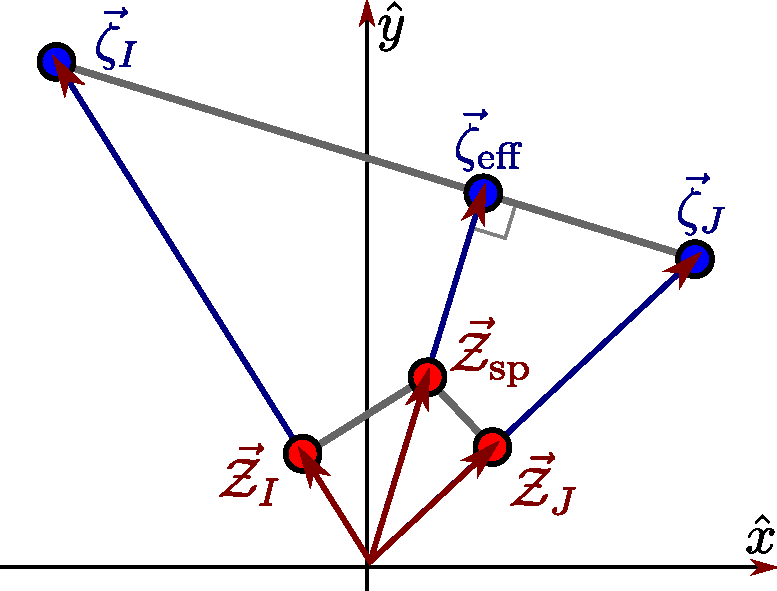
\includegraphics[width=0.4\textwidth]{mult.pdf}\label{fig:mult}
        }
        \quad
	\subfigure[]{
		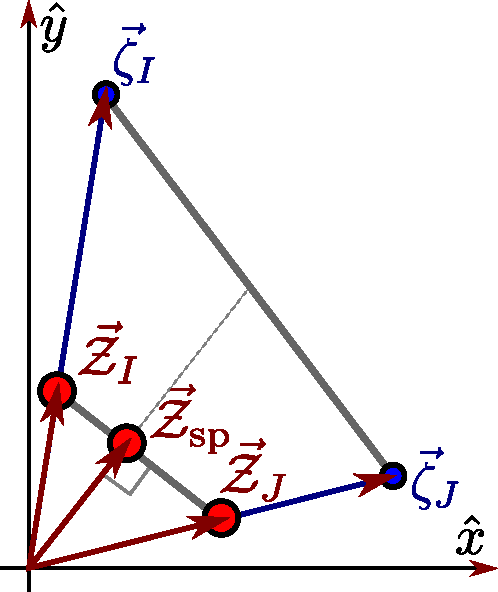
\includegraphics[width=0.3\textwidth]{add.pdf}\label{fig:add}
        }
	\caption{\small Sketch of the possible behaviour of the species scale $\Lambda_{\rm sp}$ along limits for which two (or more) leading towers become light at the same rate. Whenever there exists an effective tower $\vec{\zeta}_{\rm eff}$ of bound states, the associated \emph{multiplicative species} \textbf{(a)} dominates over the individual $\vec{\mathcal{Z}}_I$ and $\vec{\mathcal{Z}}_J$, and is perpendicular to the facet spanned by the individual towers, ${\rm Hull}(\{\vec{\zeta}_I,\vec{\zeta}_J\})$. On the contrary, if the effective towers are absent, the resulting \emph{additive species} \textbf{(b)} $\vec{\mathcal{Z}}_{\rm sp}$ is associated to the sum of the states given by each tower alone, being moreover perpendicular to ${\rm Hull}(\{\vec{\mathcal{Z}}_I,\vec{\mathcal{Z}}_J\})$ and only providing for the actual cut-off when both individual species fall at the same rate. In this case, $\vec{\mathcal{Z}}_{\rm sp}$ is not expected in general to be orthogonal to ${\rm Hull}(\{\vec{\zeta}_I,\vec{\zeta}_J\})$.}
		\label{fig:add mult}
	\end{center}
\end{figure}
%%%%%%%%%%%%%%%%%%%%%%%%%%%	

\begin{center}
	\textbf{Condition 3}: \textit{For every connected component of the space of infinite distance limits, there exists at least one direction associated to an emergent string limit or the homogeneous decompactification of an internal cycle to a higher dimensional vacuum}. 
\end{center}

With the previous two conditions, we have divided the moduli space into different regions and shown that  $\vec{\zeta}_{\rm t}\cdot\vec{\mathcal{Z}}_{\rm sp}$  remains constant across those. The only thing missing is to set this constant to  $\frac{1}{d-2}$, which occurs if there exists \emph{at least one} asymptotic direction resulting in a string perturbative limit or a decompactification to a higher dimensional vacuum. This resembles but it is a weaker condition than the Emergent String Conjecture \cite{Lee:2019wij}, as we explain in the following.

\subsubsection*{Relation to Emergent String Conjecture}

To conclude, we want to comment on the relation between the pattern \eqref{eq:pattern} and the Emergent String Conjecture (see Section \ref{s:SDC}), since they are clearly linked and one might wonder to what extent the former follows from the latter, and viceversa. In a nutshell, this conjecture holds that every infinite distance limit should either correspond to a decompactification to higher dimensions or to a perturbative limit where a critical string becomes weakly coupled and tensionless. Therefore, other potential descriptions where the lightest object corresponds to a higher-dimensional $p$-brane (with $p \geq 2$) would be thus forbidden, which has been argued to be related to the consistency of the conjecture under dimensional reduction \cite{Alvarez-Garcia:2021pxo}.
	
On the other hand, in the present section  we have identified some sufficient conditions that allow the pattern to hold universally in moduli space, so that we can compare them directly with the Emergent String Conjecture. \emph{Condition 1} does not follow from the latter, since it is actually a requirement on the asymptotic structure of the towers and how the $\zeta$- and $\mathcal{Z}$-vectors are allowed to change as we move within moduli space. \emph{Condition 3} clearly follows from it, even though it is a weaker statement. The interesting connection, however, is associated to \emph{Condition 2}, which is the most important feature underlying the pattern. A priori, it is not obvious whether the Emergent String Conjecture implies such condition, or why the latter requirement is stronger, as we explain in the following. Consider for instance some decompactification limit in which we have several Kaluza-Klein towers so that several directions open up asymptotically. If all these towers are truly Kaluza-Klein towers from the perspective of the \emph{same} duality frame, then it is guaranteed that we will populate the lattice of KK quantum numbers and thus satisfy \emph{Condition 2}. This is because for very large momenta, one can use the WKB approximation to compute the eigenvalues of the laplacian of the internal space, and they are such that the number of modes with mass smaller than or equal to some large energy $\Lambda_{\rm UV}$ scales roughly as follows
%
\begin{equation}
	N \sim \left( \frac{\Lambda_{\rm UV}}{m_{\rm KK}}\right)^n\, ,
\end{equation}
%
with $n$ being equal to the total number of decompactifying dimensions. Note that this has precisely the structure of the \emph{effective tower} (c.f. eq. \eqref{e:eff tow}) in the multiplicative species scenario, such that \emph{Condition 2} holds. However, the Emergent String Conjecture does not require a priori that the individual limits associated to each tower can be interpreted as decompactification points from the perspective of the same dual frame. For instance, in the case in which we take a limit along which a KK tower decays at the same rate than a tower of winding modes, even if both towers signal a decompactification limit towards some dual frame, they do not do so within the same duality description and therefore the total number of species is actually additive. We denote this as a case of \emph{non-compatible} decompactification limits. Hence, if we only had these two separate towers, we would not get a lattice of bound states thereof such that \emph{Condition 2} --- and consequently the pattern --- would not hold. However, in practice, whenever this scenario occurs in string theory, we always get additionally a tower of string oscillator modes precisely along the direction where the KK and winding modes decay at the same rate, so that we realize an emergent string limit (rather than decompactifying two extra dimensions), ensuring that \eqref{eq:pattern} is satisfied. This seems to be always the case even in more complicated top-down constructions, where we are not simply considering circle decompactifications and we do not have winding modes of a perturbative string but rather towers of particles coming from wrapped branes. Nevertheless, even in those cases, the rich network of string dualities always allow us to identify some critical string becoming tensionless along the interface between the different  \emph{non-compatible} decompactification limits. We want to remark that this is indeed crucial for the pattern to hold, and from a bottom-up perspective, it imposes a non-trivial constraint on how the different infinite distance limits glue together within the moduli space.
	
Therefore, if we interpret the Emergent String Conjecture as the milder claim that the leading tower must be either a Kaluza-Klein one --- in some dual frame --- or an emergent string, then it does not immediately imply \emph{Condition 2} and is strictly weaker than the pattern. For instance, the above scenario of \emph{non-compatible} decompactification limits would still be consistent with this mild version of the conjecture even if we did not have the string becoming tensionless at the interface. However, if we interpret the Emergent String Conjecture as the claim that there must be either a single dual frame where all the leading towers can be seen as KK towers or we get an emergent string providing for the leading one, then it automatically implies \emph{Condition 2}. In that case, the pattern would essentially follow from it, barring some subtleties related to the sliding of the $\zeta$-vectors, c.f. \emph{Condition 1} above. This latter possibility would be very interesting, as the pattern would then open new avenues to try to provide a bottom-up explanation for the conjecture itself, which so far has only been motivated by string theory examples.\footnote{See \cite{Basile:2023blg,Basile:2024dqq,Bedroya:2024ubj} however for recent efforts in trying to address this point.} %If we were able to provide a bottom-up rationale for the pattern (possibly based on black hole physics or entropy arguments), then we could use it to argue for the ESC and show that a consistent quantum gravity theory necessarily requires from the existence of perturbative strings and extra dimensions.
In fact, using recent results \cite{Bedroya:2024uva} which argue that asymptotically the mass scale of the lightest tower $m_{\rm t}$ can be detected as well by (neutral) black holes which undergo some phase transition, one may rewrite \eqref{eq:pattern} equivalently as follows
%
\beq\label{eq:patternblackholes}
	\frac{\vec\nabla \Lambda_{\rm BH}}{\Lambda_{\rm BH}} \cdot\frac{\vec\nabla \LSP}{\LSP}= \frac{1}{d-2}\, ,
\eeq
%
where $\ell_{\rm BH} = \Lambda_{\rm BH}^{-1}$ defines the size of the corresponding singular black hole and is such that $\ell_{\rm BH} \geq \ell_{\rm sp}$. In realistic examples taken from the quantum gravity landscape, this transition typically coincides with the one described by Gregory and Laflamme \cite{Gregory:1993vy,Gregory:1994bj} (for decompactification limits) or rather with the Horowitz-Polchinski solution \cite{Horowitz:1996nw,Horowitz:1997jc} (in the emergent string case). Hence, a bottom-up argument linking the variation over the moduli space of these two energy scales or equivalently their entropies, namely
%
\beq\label{eq:patternentropies}
	\vec\nabla \log S_{\rm BH} \cdot \vec \nabla S_{\rm BH,\, min}= d-2\, ,
\eeq
%
may serve as a good starting point for addressing this important question in the future.


\section{Summary}

In this chapter we have pointed out an interesting relation that it is satisfied in all known examples of infinite distance limits in the moduli space of string theory compactifications, regardless of the level of supersymmetry or the topology/geometry of the internal space. This pattern moreover provides a sharp connection between the asymptotic value of the variation rate (in moduli space) of the species cut-off and the mass of the leading tower of states, given by \eqref{eq:pattern}. We checked that it holds for multi-field geodesic trajectories where several moduli are taken to infinity at the same time, even if the species scale is not only determined by the leading tower of states but captures information of other subleading ones. 
	
At the very least, it can be regarded as a common thread underlying all known string theory examples that have been explored so far, and makes manifest the very constrained structure behind the vast casuistics of different types of infinite distance degenerations, as well as how they can fit together in a given moduli space. We suspect, though, that the universality of a relation like \eqref{eq:pattern} is rooted in a deeper underlying quantum gravity principle, rather than being just a lamppost effect of all known string constructions. Hence, an important step forward in our understanding of the pattern would be to search for a purely bottom-up rationale that could explain the latter independently of string theory. Promising avenues along this direction include phrasing the problem in terms of black holes or holographic entropy bounds (c.f. eqs. \eqref{eq:patternblackholes} and \eqref{eq:patternentropies}), since the pattern seems to relate two different special scales in black hole physics \cite{Bedroya:2024uva}. Alternatively, one could also think of the number of species as a measure of the density of states in any theory coupled to Einstein gravity, so that the less dense the tower is, the faster it can become light according to \eqref{eq:patternN}. Another interesting direction would be to use S-matrix bootstrap techniques, since the species cut-off can be understood as the scale at which the semi-classical Einstein gravity description breaks down and higher-derivative terms start dominating over the tree-level Einstein term, see Chapter \ref{ch:Higherdimops}. It would be fantastic if one could derive a precise link between $\LSP$ and e.g., the scale of the first massive spin-2 field of some Kaluza-Klein tower.
	
In a similar vein, one could argue that in fact finding the physics behind the pattern would presumably have profound consequences for the Swampland program, since it implies a refined formulation of the Distance conjecture that constrains the nature of the towers and imposes a sharp bound on how fast it becomes light. Indeed, if the pattern holds then it automatically implies a lower bound on the exponential rate of the tower given by $\lambda_{\text{t}} \geq \frac{1}{\sqrt{d-2}}$, which supports the idea put forward in \cite{Etheredge:2022opl} and it is closely related to the Emergent String Conjecture \cite{Lee:2019wij}. Relatedly, the relation \eqref{eq:pattern} also constrains the exponential decay rate of the species cut-off, whose convex hull condition (c.f. also Chapter \ref{ch:bounds}) becomes dual --- in the polytope sense --- to the one imposed on the towers. Furthermore, it provides a clear recipe to determine the species scale upon knowledge of the leading tower of states along different directions. It would be equally interesting to explore how it could be extended to the interior of the moduli space, where the notion of a leading tower of states is no longer well-defined.\footnote{See \cite{Rudelius:2023spc,Bedroya:2024uva} for recent attempts along this direction.}
	
As a byproduct, we identified in Section \ref{s:bottomup} three sufficient conditions that the towers of states and the asymptotic geometry in moduli space must satisfy to allow for the pattern to hold. Interestingly, the most important condition resembles a sort of (sub-)Lattice WGC where the role of the gauge charges is played by the levels of the towers. This condition also follows from a strong interpretation of the Emergent String Conjecture. Hence, many ideas in the Swampland program get interconnected and can be re-derived from this simple equation relating the variation of the species scale and the leading tower of states becoming light asymptotically. 



%%%%%%%%%%%%%%%%%%%%%%%%%%%%%%%%%%%%%%%%%%%%%%%%%
%%%%%%%%%%%%%%%%%%%%%%%%%%%%%%%%%%%%%%%%%%%%%%%%%

%%%%%%%%%%%%%%%%%%%%%%%%%%%%%%%%%%%%%%%%%%%%%%%%%
%%%%%%%%%%%%%%%%%%%%%%%%%%%%%%%%%%%%%%%%%%%%%%%%%

%%%%%%%%%%%%%%%%%%%%%%%%%%%%%%%%%%%%%%%%%%%%%%%%%
%%%%%%%%%%%%%%%%%%%%%%%%%%%%%%%%%%%%%%%%%%%%%%%%%


